%%
%% THESIS/DISSERTATION TEMPLATE FOR FLORIDA POLYTECHNIC UNIVERSITY
%%
%% This example is written by Chris Kelley, edited from a template for the University of Alabama. 
%%

%% Use the fputhesis document class
\documentclass[thesis]{fputhesis}



%% Basic packages you'll probably want to use.
\usepackage{graphicx}                 %% For using \includegraphics{}
%\usepackage{subfigure}
\usepackage{float}
\usepackage{amsmath}
\usepackage{multirow}
\usepackage{color}                    %% For colors used in listings.
\usepackage{listings}                 %% Code listings (for engineers)
\usepackage[numbers, sort]{natbib}
\usepackage[table,xcdraw]{xcolor}
\usepackage{caption}
\usepackage{subcaption}

\usepackage[normalem]{ulem}
\useunder{\uline}{\ul}{}
\usepackage{longtable}

\newcommand{\Vol}{\rotatebox[origin=c]{180}{\ensuremath{A}}}

%% Includes
\newacronym{ar}{AR}{Augmented Reality}
\newacronym{vr}{VR}{Virtual Reality}
\newacronym{xr}{XR}{eXtended Reality}
\newacronym{hud}{HUD}{Heads-Up Display}
\newacronym{api}{API}{Application Programming Interface}
\newacronym[longplural={Central Processing Units}]{cpu}{CPU}{Central Processing Unit}
\newacronym[longplural={Graphics Processing Units}]{gpu}{GPU}{Graphics Processing Unit}
\newacronym[longplural={Personal Digital Assistants}]{pda}{PDA}{Personal Digital Assistant}
\newacronym{sdk}{SDK}{Software Development Kit}
\newacronym{fps}{FPS}{Frames per Second}
\newacronym{ui}{UI}{User Interface}
\newacronym{ux}{UX}{User eXperience}
\newacronym{mar}{MAR}{Mobile Augmented Reality}
\newacronym{fov}{FoV}{Field of View}
\newacronym{tam}{TAM}{Technology Acceptance Model}
\newacronym{pwa}{PWA}{Progressive Web App}
\newacronym{os}{OS}{Operating System}
\newacronym{yolo}{YOLO}{You Only Look Once}
\newacronym{csv}{CSV}{Comma-Separated Values}
\newacronym{aws}{AWS}{Amazon Web Services}
\newacronym{db}{DB}{Database}
\newacronym{tls}{TLS}{Transport Layer Security}
\newacronym{ssl}{SSL}{Secure Socket Layer}
\newacronym{ai}{AI}{Artificial Intelligence}
\newacronym{tlx}{TLX}{Task Load Index}
\newacronym{sus}{SUS}{System Usability Scale}
\newacronym{e}{E}{Effort}
\newacronym{fr}{FR}{Frustration}
\newacronym{md}{MD}{Mental Demand}
\newacronym{p}{P}{Performance}
\newacronym{pd}{PD}{Physical Demand}
\newacronym{td}{TD}{Temporal Demand}
% thanks to http://tex.stackexchange.com/a/47579/71109
\usepackage{ifxetex}
\usepackage{ifluatex}
\newif\ifxetexorluatex % a new conditional starts as false
\ifnum 0\ifxetex 1\fi\ifluatex 1\fi>0
   \xetexorluatextrue
\fi

\ifxetexorluatex
  \usepackage{fontspec}
\else
  \usepackage[T1]{fontenc}
  \usepackage[utf8]{inputenc}
  \usepackage[lighttt]{lmodern}
\fi

\usepackage{textcomp}
\usepackage{xcolor}
\usepackage{listings}
\usepackage{upquote}

\definecolor{keyword}{HTML}{2771a3}
\definecolor{pattern}{HTML}{b53c2f}
\definecolor{string}{HTML}{be681c}
\definecolor{relation}{HTML}{7e4894}
\definecolor{variable}{HTML}{107762}
\definecolor{comment}{HTML}{8d9094}
\definecolor{background}{HTML}{ededed}

\lstset{
        backgroundcolor=\color{background},
	numbers=none,
	stepnumber=1,
	numbersep=5pt,
        numberstyle=\tiny\color{background},
	basicstyle=\small\ttfamily,
	keywordstyle=\color{keyword}\bfseries\ttfamily,
	commentstyle=\color{comment}\ttfamily,
	stringstyle=\color{string}\ttfamily,
	identifierstyle=,
	showstringspaces=false,
	aboveskip=3pt,
	belowskip=3pt,
	columns=flexible,
	keepspaces=true,
	breaklines=true,	
	captionpos=b,
	tabsize=2,
	frame=none,
}

\lstset{upquote=true}

\lstdefinelanguage{cypher}
{
	morekeywords={
		MATCH, OPTIONAL, WHERE, NOT, AND, OR, XOR, RETURN, DISTINCT, ORDER, BY, ASC, ASCENDING, DESC, DESCENDING, UNWIND, AS, UNION, WITH, ALL, CREATE, DELETE, DETACH, REMOVE, SET, MERGE, SET, SKIP, LIMIT, IN, CASE, WHEN, THEN, ELSE, END,
		INDEX, DROP, UNIQUE, CONSTRAINT, EXPLAIN, PROFILE, START,
	}
}


\newcommand{\mycdots}{\cdot\!\cdot\!\cdot}

\lstset{language=cypher,
	literate=*
	{...}{$\mycdots$}{1}
	{theta}{$\theta$}{1}
    }
\usepackage{ifxetex}
\usepackage{ifluatex}
\newif\ifxetexorluatex % a new conditional starts as false
\ifnum 0\ifxetex 1\fi\ifluatex 1\fi>0
   \xetexorluatextrue
\fi

\ifxetexorluatex
  \usepackage{fontspec}
\else
  \usepackage[T1]{fontenc}
  \usepackage[utf8]{inputenc}
  \usepackage[lighttt]{lmodern}
\fi

\usepackage{textcomp}
\usepackage{xcolor}
\usepackage{listings}
\usepackage{upquote}

\definecolor{keyword}{HTML}{2771a3}
\definecolor{pattern}{HTML}{b53c2f}
\definecolor{string}{HTML}{be681c}
\definecolor{relation}{HTML}{7e4894}
\definecolor{variable}{HTML}{107762}
\definecolor{comment}{HTML}{8d9094}
\definecolor{background}{HTML}{ededed}

\lstset{
        backgroundcolor=\color{background},
	numbers=none,
	stepnumber=1,
	numbersep=5pt,
        numberstyle=\tiny\color{background},
	basicstyle=\small\ttfamily,
	keywordstyle=\color{keyword}\bfseries\ttfamily,
	commentstyle=\color{comment}\ttfamily,
	stringstyle=\color{string}\ttfamily,
	identifierstyle=,
	showstringspaces=false,
	aboveskip=3pt,
	belowskip=3pt,
	columns=flexible,
	keepspaces=true,
	breaklines=true,	
	captionpos=b,
	tabsize=2,
	frame=none,
}

\lstset{upquote=true}

\lstdefinelanguage{JavaScript}{
  morekeywords=[1]{break, continue, delete, else, for, function, if, in,
    new, return, this, typeof, var, void, while, with},
  % Literals, primitive types, and reference types.
  morekeywords=[2]{false, null, true, boolean, number, undefined,
    Array, Boolean, Date, Math, Number, String, Object},
  % Built-ins.
  morekeywords=[3]{eval, parseInt, parseFloat, escape, unescape},
  sensitive,
  morecomment=[s]{/*}{*/},
  morecomment=[l]//,
  morecomment=[s]{/**}{*/}, % JavaDoc style comments
  morestring=[b]',
  morestring=[b]"
}[keywords, comments, strings]

\lstset{language=Javascript,
	literate=*
	{...}{$\mycdots$}{1}
	{theta}{$\theta$}{1}
    }
\makeglossaries
% TODO: If you have any special commands defined, include them here.
\usepackage[titletoc]{appendix}%
\usepackage[hidelinks]{hyperref}
\usepackage[super]{nth}
\usepackage{siunitx}
\usepackage{array}
\usepackage{booktabs}
    \setlength\heavyrulewidth{0.20ex}
    \setlength\cmidrulewidth{0.10ex}
    \setlength\lightrulewidth{0.10ex}
    \newcommand{\ra}[1]{\renewcommand{\arraystretch}{#1}}

\sisetup{detect-weight,mode=text,round-mode=places,round-precision=4}
% for avoiding siunitx using bold extended
\renewrobustcmd{\bfseries}{\fontseries{b}\selectfont}
\renewrobustcmd{\boldmath}{}
% abbreviation
\newrobustcmd{\B}{\bfseries}
% shorten the intercolumn spaces
\addtolength{\tabcolsep}{4.1pt}

%% Required parameters (these default to undefined)
\author{Colter Roche}       %% Your name!
\university{Florida Polytechnic University}
\gradyear{Fall \the\year}
\place{Lakeland, Florida}
\degree{Master of Science in Computer Science}   %% Change to suit your degree.
\prevdegree{Bachelor of Science, Computer Science}   %% Change to suit your previous degree.
\department{COMPUTER SCIENCE}   %% Change to suit your department.




%% The people on your committee.
\adviser{Dr. A. Hamam}   %% Your adviser/committee chair!\
\memberA{Dr. M. Abid}
\memberB{Dr. O. Toker}
\provost{Dr. B. Thiessen} %% ***ahamam *** use Dr. Parker name here



%% Note the use of \and to create line breaks and the
%% inverted pyramid style requested by the graduate school.
%% You have to do this manually. Sorry.
\title{Item-FindAR: Improving Consumer Awareness \and
  through Mobile Augmented Reality \and
  on the Web}



%% These are body text paragraphs to be placed in the front matter.
\abstract{
Consumers face multiple challenges while shopping for products in a grocery or pharmacy setting, including illegible or inconsistent labels, mislabeled ingredients and allergens, and densely stocked shelves of similarly packaged items. This thesis describes the development of Item-FindAR, a \acrfull{mar} system designed to streamline the shopping process. Our system allows users to easily find items and obtain consistent product information without direct physical contact, via virtual information overlays on a mobile device display.

The research aimed to create a platform-independent solution that users could access via their smartphone browsers, removing the need for costly or specialized equipment. We integrated a YOLOv8 object detection model for markerless tracking with WebXR, utilizing the recently released raw-camera-access feature to access the user's smartphone camera in real time. We then processed the image remotely to reduce resource usage. The development involved multiple iterations of design, build, and testing, resulting in a working prototype that leverages computer vision to recognize and locate items in the user’s environment, with relevant information displayed over the product's image.

Two user studies were conducted to evaluate the system's usability and user satisfaction. Results indicate that Item-FindAR enhances the shopping experience by simplifying product identification and delivering essential information in a user-friendly manner. The research also underscores the significance of user comfort and data security, suggesting that these aspects are crucial for the widespread adoption of \acrshort{mar} technologies in retail.

This thesis contributes to the field of \acrlong{mar} by offering valuable insights into the creation of web-based AR applications reliant on custom computer vision models, presenting a complete client, server, database, and set of object detection models.
}

%\dedication{
%Type or input{} your dedication here.
%}

\acknowledgments{
Thank you Dr. Hamam for serving as my advisor during this extended program. Your patience and support has been invaluable through the many ups and downs of this research endeavor. Thank you as well to Ms. Emily Lowers, Florida Polytechnic's Graduate Program Coordinator, whose constant support and help with extensions made the completion of this thesis possible. Thank you to Dr. M. Abid for the excellent classes on classical computer vision, they helped to solidify my understanding of the fundamentals and shaped my perspective for this project. Despite the short notice, Dr. Abid, Dr. O. Toker, and Dr. B. Thiessen agreed to serve on the new graduate committee, for which we are very grateful. I would also like to thank Dr. O. Topsical, Dr. D. Demirel, and Dr. B. Chandrasekaran, the members of my previous graduate committee, for their time and support, and wish them well in their future careers. 

Thank you to all the students that participated in the user studies, with special thanks to the participants in the first study for their comments on how to improve our system. This feedback was invaluable in the design process for the second version. Thank you Ms. Rochelle Picard, for providing access to the Mosaic Cafe, helping me take photos of the items, and helping to keep the cafe open over the summer months. We hope the data and models we compiled will be useful to future students who may continue research in partnership with the Cafe. Thanks as well to Matt and Randy for their warm attitudes and cold drinks, many a coffee and tea were bought during the process. This thesis would not have been possible without the support of all these people, plus the many more who have helped to shape my development at this university.

Finally, a huge thank you to my parents, James and Mauria Roche, for their ongoing support and love during my nine years at Florida Poly. 
}



\begin{document}

%% Makes the title, abstract, dedication, table of contents, etc.
%% Must be before \begin{body}
\makefrontmatter

%% BODY PORTION
%% The bulk of your thesis.
%% Begin your \chapter's here.

\begin{body}

%% Body chapters.
\chapter{INTRODUCTION}
Product labels are the consumer's main method of assessing food and drug products before purchasing items, and convey a range of information including content, nutritional information, branding, testimonials, and a wide range of other information to persuade or attract buyers \cite{nute_product_2019}. Manufacturers often produce labels that are confusing or difficult to read, however. A study of 100 Canadian product labels found that only 7\% of the labels were rated as "Easy to read" \cite{mackey_ease_2009}, and another study found that parents of children with food allergies had a very difficult time correctly identifying whether a product contained a specific substance \cite{joshi_interpretation_2002}. Specific products may also be difficult to identify when arranged on store shelves, as there are many similar products that may surround the user's sought after item. A range of factors influence shelf placement including product sales, customer satisfaction, and company contracts \cite{sun_segmentation_2019}. This situation can be substantially improved for the consumer by augmenting the physical reality that they view when scanning a food or drug display.


\acrfull{ar} refers to the merging of physical reality and virtual objects via an overlay medium. Unlike virtual reality, which immerses the user in a different environment for educational or entertainment purposes, \acrshort{ar} serves to provide additional information and content embedded in the user's surroundings. \acrshort{ar} experiences can be context aware, logically placing and positioning virtual objects as if they were real, or simply provide textual information overlaid on a visual of the environment, similar to a \acrlong{hud}. \acrshort{ar} devices traditionally consist of either a glasses-type hardware format, with content displayed on a transparent panel, or a VR type headset with cameras to display a live feed of the environment. These devices tend to be unaffordable for the average person. With the rise of popular apps like Pokemon Go or Snapchat, smartphone users have grown more accustomed to \acrshort{ar} experiences on their mobile devices. Utilizing the phone's included gyroscope and cameras, APIs exist for both Apple and Android devices that allow for developers to track the device's location in physical space and align and place virtual objects in real world space with accurate scaling and stable positioning.

\section{Motivation and Goals}
The major difficulties we intend to address with this thesis are finding specific items on crowded shelves, and providing readable, standardized product information without the user needing to touch items directly. \acrshort{ar} allows us to overlay information on products directly without obscuring the labels, addressing the latter, while advances in computer vision models allow for the rapid recognition and and tracking of items in the user's space. The broad goals for our system included:
\begin{enumerate}
    \item Broad smartphone support regardless of hardware
    \item Users can easily access general information on items visible
    \item Users can search for specific items
    \item Users can avoid physical contact with the items on display
\end{enumerate}
Based on these goals, we devised a set of functional and performance requirements for a system that would fully address the relevant concerns: The application should utilize a client/server architecture to provide users with a shopping tool accessible from their phone's browser, capable of identifying products, highlighting their location on the shelf, providing simplified product and nutritional information, and allowing users to compare items without the need for traditional web searches. The system uses machine learning to recognize products without special markers and overlay information in a clear and readable fashion. 

\section{Preliminary Research}
Prior to this thesis, research on the development and use of a marker-based product identifier using Microsoft's HoloLens was conducted by one of the authors of this work and a previous student at the university\cite{souza-herod_augmented_2021} . This section provides a brief overview of the findings of that research and how they affected the functional requirements for our prototype.

The previous research centered around developing an application for identifying pharmaceutical products and presented the user with options to view a product description, expiration date, and product reviews. The application was developed using Unity and Vuforia, a proprietary \acrshort{ar} library. The user interface was designed for the gesture controls supported by the HoloLens; users were presented with buttons and could "tap" in the air to select them. Users could also adjust the size of the text. Products were identified using Vuforia's marker system, requiring each item class to have a unique code. Stickers were then applied to the bottles, allowing the headset to recognize items and position information over them. Information for the items was stored remotely in a \acrfull{db} to be queried by the headset upon recognition. 

\begin{figure}[h]
    \centering
    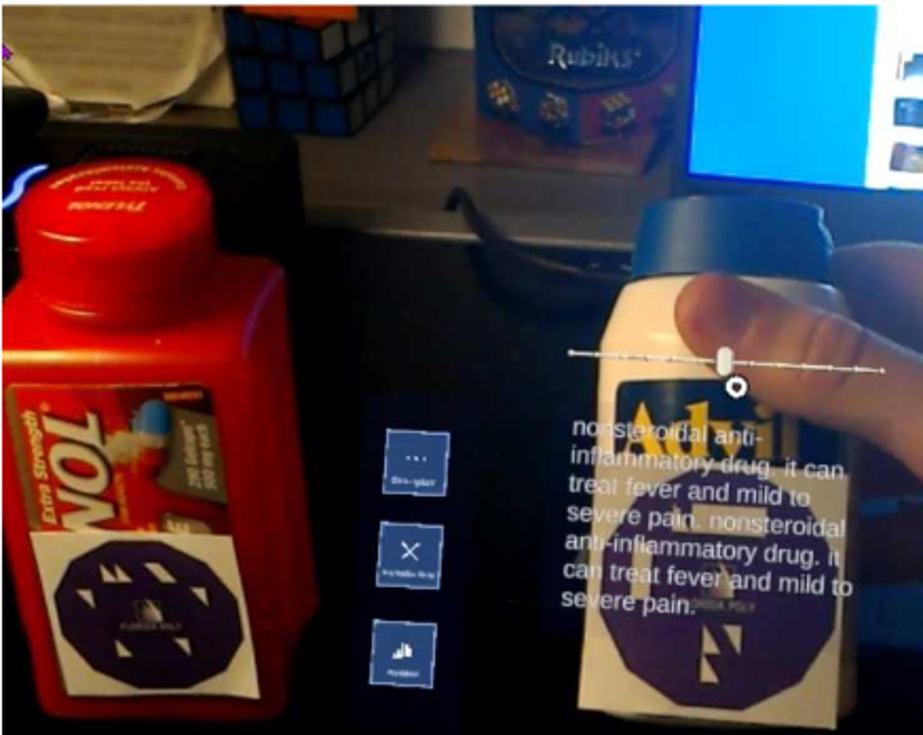
\includegraphics[width=0.6\linewidth]{Images/hololens work.png}
    \caption{Previous system with markers and HoloLens UI}
    \label{fig:hololens-work}
\end{figure}

There were two major issues we wanted to address from the previous system: item markers and hardware availability. Vuforia is simple to use but expensive, and has unacceptable limits on recognition totals and classes. Marker-based systems also require external markers to be applied, requiring businesses to apply an extra sticker or other marker. Apps that scan item barcodes and provide data already exist, but require users to pick up items to access the code. Some users may have difficulty reaching items, and scanning items from a distance could help reduce congestion in stores. Eliminating this and directly recognizing the items allows for use anywhere the system can detect products. Systems that require external support in the form of access to store databases or beacon systems for navigation limit the user's ability to utilize the application when they might need it, for example, in their home or at an unsupported store.

Our second concern was redeveloping the application and interface for a mobile device instead of the HoloLens. Microsoft's headset allows for a more immersive experience, at a prohibitive cost to the average consumer. The headset also has comfort and long-term wear issues. We wanted to eliminate the expense, discomfort, and inconvenience of using a headset, and allow for cross-platform user access. 

This led us to favor web applications that run in a device's browser, theoretically eliminating the need for platform specific development. \acrfull{ar} web app development is a relatively unexplored field, however, and access the camera image in real time from the web was an emerging capability. Chromium (the basis for Google's Chrome browser) hadn't implemented the new standard until December of 2022, and Chrome is currently the only mobile browser to properly support \verb|raw-camera-access|. Despite the newness of the technology, we chose to pursue a web app architecture and selected the open source standard WebXR for our implementation.  We considered the benefits of our novel approach to outweigh the risk of utilizing emerging technologies, as the increase in knowledge related to web-based \acrshort{ar} outweighed the increased difficulty or risk of failure.
\filbreak
\section{Research Questions}
The main research question is: \textit{Can the grocery shopping experience be improved via the use of Mobile Augmented Reality, specifically finding and identifying and displaying the contents of products in an accessible manner to consumers?}
To sufficiently answer the main question, several related questions need to be answered:
\begin{itemize}
    \item Can items be recognized without third-party identifiers?
    \item What steps are needed to ensure user data is protected?
    \item How can we maximize the comfort of users to encourage them to use our system?
    \item What is needed to ensure consistent performance across devices?
    \item How familiar are potential users with other Augmented Reality applications?
\end{itemize}
\section{Methodology}
Our primary method for answering the questions above was an iterative design process consisting of three steps: 
\begin{enumerate}
    \item Create a list of requirements by analyzing past results
    \item Develop and implement a prototype
    \item Test the prototype and gather user feedback
\end{enumerate}
We repeated these steps twice, developing and testing two versions of our system. The first was a rough proof of concept, capable of identifying and locating items but lacking many of the functional requirements identified. After user testing, we continued development and produced a complete version that met the full list of requirements and performed another user study. The results from both studies were compared and analyzed, and a set of key features for the best user experience are included in Chapter 5.
\section{Contributions}
\begin{itemize}
    \item {Two published papers:
    \begin{itemize}
         \item []{\textbf{Augmented Reality Shopping System and Experience: Overview of the Literature}\cite{roche_augmented_2023}}
         \item []{\textbf{Mobile Augmented Reality Shopping System}\cite{roche_mobile_2023}}
    \end{itemize}
    }
    \item Compiled data for 133 items offered at the University's Mosaic Cafe
    \item Graph-based database for the 133 items
    \item Partial annotated computer vision training set for 133 items
    \item Fully annotated training set for 12 items in the University lab and other locations
    \item Code and documentation for how to access the camera image while using Three.js (web rendering engine library)
    \item Code and documentation for how to align virtual markers with real-world objects in a web context
    \item Functional final prototype
\end{itemize}

\section{Thesis Structure}
This introductory chapter serves as an overview of what led to the creation of this thesis and what topics are covered in subsequent chapters. The second chapter covers past research on augmented reality for shopping, and an analysis of challenges related to markerless item recognition. The third and fourth chapters describe the multi-stage development and testing process for our application prototype, the fifth presents the results and discusses how to interpret them, and chapters 6 \& 7 answer the research questions, draw conclusions from the work, and covers future research.

\chapter{LITERATURE SURVEY}
This chapter provides an overview of previous work described in the literature related to the major elements of our proposed \acrfull{ar} shopping application. 
\section{Previous Work on \acrshort{ar} Shopping Apps}
Several systems have been developed that attempt to address the common issues involving finding items when shopping in grocery stores. ProFI \cite{li_profi_2013} was a shopping cart mounted product finding system designed to help users find items on shelves. The researchers found that highlighting or circling items on the shelf greatly improved search effectiveness, but the system lacked flexibility and required that all the data and processing be done on the device, limiting the number of detectable products. Ahn et al. \cite{ahn_supporting_2015} had a different approach, creating a mobile phone application that provided users with nutritional information for sections of the shelves rather than individual items. Images of the aisle from the user's phone were sent to a cloud server for identification, and then the user's location in the store was identified using the store's product catalog. Users found the presentation of nutritional data to be useful for their shopping experience, but the application required access to the store's product database which restricted usability significantly. Jayananda et al.\cite{jayananda_augmented_2018} took a similar approach using Bluetooth identifiers (beacons) for navigation and product recognition to provide nutritional data to users. 
\filbreak
The CoShopper system presented by Alhamdan et al. \cite{alhamdan_extended_2020} detailed the development of a similar shopping \acrshort{ar} system for smart glasses that 
includes personalized nutrition information for the user but did not help them locate the item on shelves. ARMart \cite{roddiger_armart_2018} implements an item categorizer and search function with color coded overlays directly on the box label, but was limited to only working on rectangular labels and having a limited, locally stored database of items. Xia et al. \cite{xia_parashop_2020} created an \acrshort{ar} shopping guide for those on the autism spectrum to help with visual list-making, item identification, and helpful 
reminders for different steps of the shopping experience. Their system relied heavily on barcodes, however, only capable of recognizing produce items without a barcode. 

Our \acrshort{ar} system builds upon previous work at Florida Polytechnic from Souza-Herod \cite{souza-herod_augmented_2021} on a marker-based shopping assistant for Microsoft's HoloLens. That system used unique markers to identify medicines and provide product information and dosage in a larger, more readable format. Our proposed system improves upon these features by eliminating the need for markers and changing the device to a generally accessible smartphone or tablet. 

\section{Mobile \acrshort{ar} Frameworks and Object Tracking}
\acrfull{ar} solutions are available on three major hardware platform types currently: smart glasses or headsets, mobile phones and tablets, or traditional notebook or desktop computers. Now that smartphones are commonplace, the average user carries around everything they need for an \acrshort{ar} experience. Many phones have multicore \acrfullpl{cpu}, dedicated \acrfullpl{gpu}, and high speed networking, allowing for faster processing \cite{chatzopoulos_mobile_2017}. Google's ARCore, Apple's ARKit, and Vuforia all provide native functionality for tracking the device's position in space relative to their surroundings, anchoring digital augmentations to specific spots, marker recognition, and environment processing \cite{oufqir_arkit_2020}.

The simplest form of object tracking and augmentation is marker based, with printed, high contrast identification labels that the software detects via a device camera. This tracking 
method requires an unobstructed view of the marker, limiting the user's ability to interact with items in the scene and possibly obstructing parts of the scene depending on placement \cite{platonov_mobile_2006}. Markerless detection addresses these issues by eliminating the need for unique markers and allowing for more robust methods for interaction including hand gestures that occlude part of the tracked object \cite{bai_poster_2013}. 
This method has a significantly higher computational cost, relying on complex computer vision or machine learning algorithms to detect and recognize object based on pattern and shape. The high computational cost generally makes markerless tracking too inefficient for use on lower-end devices without heavy optimization \cite{nazri_current_2014}, due to memory and processor usage. The other main challenge stems from limited screen space, reducing the \acrfull{fov} for augmentation and increasing the need for input methods beyond onscreen buttons.

\section{Client/Server Architecture for \acrshort{ar}}
Offloading heavy computational tasks to another device with greater processing and storage capabilities is a promising option for improving \acrshort{ar} performance on mobile devices. One method is to use a cable as a tether, or carry a separate computing unit on the user's person, but neither of these options are safe or feasible in working 
environments \cite{platonov_mobile_2006}. Running the algorithms on a remote server in the cloud eliminates the disadvantages of directly tethering, at the cost of latency issues that degrade performance if not addressed \cite{zhang_networking_2017}.

In 2003, Pasman and Woodward \cite{pasman_implementation_2003} proposed a mobile \acrshort{ar} system for \acrfullpl{pda}, featuring a server with ARToolkit to handle the tracking and rendering, which then sent the augmented frame back to the \acrshort{pda} client. Similarly, Miranda et al. \cite{miranda_low-cost_2021} developed a system for multiple users with low-end mobile devices to collaborate together by offloading both the tracking and all the rendering to a remote server.  

As the computing power of handheld devices has improved and native \acrshort{ar} \acrshortpl{api} have become more advanced, the amount of remote processing necessary is reduced. Gammeter et al. \cite{gammeter_server-side_2010} presented a client/server system for \acrshort{ar} where object recognition is handled by a high-performance server, while the client handles the object and scene tracking, allowing the recognition of millions of different objects and locations without markers or the need for large data models on the client device. A similar system capable of recognizing millions of target items and images utilized a bag of words model adapted for images running on a server and performing the rest of the necessary tracing on the client device \cite{ha_real-time_2011}. Chiu \cite{chiu_cloud_2014} proposed an \acrshort{ar} system capable of tracking and recognizing pages in a picture book while simultaneously tracking hand gestures for interaction. Object detection and tracking was performed on the phone, while the recognition and finger tracking was processed on the server. Processing and response time were compared for the cloud supported version and the device only version, with a significant boost in speed for the cloud version. These results were later confirmed for a more advanced hand tracking system \cite{chiu_interactive_2018}, with close to an eight-fold improvement.

\subsection{5G and Edge Computing}
Offloading the complex and resource intensive parts of augmented reality systems to cloud-based hardware solves the issue of resource drain on mobile devices, but introduces issues related to network speed and latency, leading to possible drops in 
quality of experience for the end user \cite{zhang_networking_2017}. Widespread adoption of 5G technology brings high bandwidth communications to the general populace, while edge computing reduces the network distance by utilizing powerful hardware on the
same network as the client devices rather than sending the data to a remote host \cite{qiao_web_2019}. Zhang et al. \cite{zhang_networking_2017} tested and assessed multiple commercial cloud \acrshort{ar} \acrfullpl{sdk} and found that they performed well, but the average latency to return a processed frame was longer than the duration between frames in a video feed captured at 30 \acrfull{fps}. They conclude that despite the latency issues, offloading the heavy computation to either a remote or edge cloud server is necessary for a smooth experience on mobile devices. 5G and edge cloud deployment are currently outside the scope of our proposed system; however, they provide avenues for future work should our method suffer from excessive latency. 

\section{\acrshort{ar} User Experience}
Users may have a sense of familiarity with smartphone-based \acrshort{ar} experiences, but issues with cognitive overload and a limited amount of space for \acrfull{ui} interactions make user experience design complex \cite{kourouthanassis_demystifying_2015}. Olsson et al. \cite{olsson_expected_2013} conducted a study of user expectations of \acrshort{ar} systems in a retail context and found that the most important information users wanted were 
product information including source location and materials, feedback from other users or instructions on use, and the ability to meaningfully compare their product of interest with other items. Participants also expressed interest in context aware suggestions such as showing the location of other relevant items or making suggestions based on previous choices. 

Ganapathy et al. \cite{ganapathy_mar_2011} produced a study to identify what users considered an acceptable delay when retrieving data from a search and found there was a range of times from 5 to 8 seconds that users found most favorable. When the load time was slower users felt the delay was too long, and when the search took less than a second users felt the search was too fast. The off-device processing that our system performs also produces search results, and we hoped this favorable range for a delay in search time would predispose users to accepting the delays due to network speed. 

Whether users feel their data is protected also has a major effect on the user experience. Augmented reality requires the use of the device camera to record video of the environment or even of the user themselves. A clear presentation of how that data will be used and stored contributes to the user's willingness to use the app. Harborth and Pape \cite{harborth_investigating_2021} found that app permissions and download count are also major factors considered by users when deciding whether an \acrshort{ar} app is safe. Poushneh \cite{poushneh_augmented_2018} found that many users judge whether an \acrshort{ar} app is safe during the account registration step, often before the \acrshort{ar} experience begins.
Users also cared greatly and expressed more engagement and preference for \acrshort{ar} experiences that allowed them to interact with the information presented in a meaningful way or augmented their abilities (i.e., testing makeup, trying on sunglasses, car user manual overlay) \cite{poushneh_augmented_2018}. 

Several factors contribute to the difficulty of designing \acrfull{mar} experiences. The necessity of holding the device in one hand limits the user's ability to interact with the screen, and the small screen size reduces the space available for data representation, often resulting in a layered approach where the user can choose to disregard information they don't need \cite{kourouthanassis_demystifying_2015}. Lee et al. \cite{lee_ar_2012} quantified this by adapting Wasson's AEIOU principles \cite{wasson_ethnography_2000} to better suit \acrfull{mar}:
\begin{itemize}
    \item \textbf{A - Activities} allow users to reach their goal
    \item \textbf{E - Environment} is where the experience takes place
    \item \textbf{I - Interactions} are the main component of Activities and include screen input or gestures
    \item \textbf{O - Object} is the mobile device and the features it provides
    \item \textbf{U - Users} are the people performing the activities and interacting with the experience
\end{itemize}

This framework provides a way to analyze and quantify individual aspects of the MAR user experience design process. A different, holistic approach to calculating the effectiveness of the MAR user experience with an accompanying \acrfull{ux} evaluation procedure, with a robust set of data collection methods including questionnaires and EEG monitoring of engagement \cite{satti_holistic_2019}. Irshad et al. \cite{irshad_design_2020} proposed and developed a similar framework for use during the early design and implementation phases of development, allowing developers to plan specific features while still considering how they'll interact and overlap with other parts of the application. They found that users thought the application they designed was appealing and novel, but wished for more consistency and efficiency. Dabor \cite{dabor_design_2019} presents a \acrshort{mar} \acrshort{ux} framework designed around minimizing the cognitive load of users. Guidelines include making sure the \acrshort{ui} is simple for both new and advanced users, minimizing the short-term memory requirements of users, and presenting information in a clear and readable way. Berman and Pollack \cite{berman_strategies_2021} created a set of guidelines and steps that cover the entire design process, including the early design and decision-making steps, i.e. what type of \acrshort{ar} application to design and how to assess what the target markets are. 

\section{User Acceptance of \acrshort{ar}}
There are many studies and reports on user experience for specific \acrshort{ar} applications, but few surveys of what users think about \acrshort{ar} in general or what issues they care about. Thomas and Holmquist \cite{thomas_is_2021} conducted a survey of how users feel about \acrshort{ar} and what their concerns are, and found that for users of \acrshort{ar} the main concerns were: 
\begin{itemize}
    \item Screen size and low \acrshort{fov} lead to less immersion
    \item Fatigue from holding a phone for long periods
    \item Device battery duration
    \item User data privacy and security
\end{itemize}
The authors conclude that more research needs to be done and that generalized surveys and studies of \acrshort{ar} use are needed, especially to identify user sentiment and to encourage broader adoption. 

Several \acrfullpl{tam} have been developed for assessing how willing and able users are to adopt an \acrshort{ar} application as part of their workflow. Schuster et al. \cite{schuster_user_2020} developed an \acrshort{ar} acceptance model based 
on the UTAUT model first proposed by Venkatesh \cite{venkatesh_user_2003}. They produced an \acrshort{ar} application designed to aid users in the construction of a toy vehicle, and then conducted tests in a real world setting, followed by a questionnaire. Analysis of the questionnaire showed that the \acrshort{ar} application shortened the time users needed to complete the task, and they found that their model was generally applicable except for a few hypotheses that needed to be rethought to better reflect user perception. 

Meyer et al. \cite{meyer_evaluating_2021} performed an acceptance case study under similar circumstances (assembling parts in a user creation space), utilizing a web-based \acrshort{mar} application. They found that users were eager to use the application and that many of the users interviewed found the application to be a useful aid in their work. Users also praised the ease of use and the lack of need for installation of the application on their device. Most of the complaints were due to technical limitations in the Web-based Augmented Reality (WebXR) framework regarding room tracking.

Koutromanos et al. \cite{koutromanos_mobile_2021} proposed and tested an \acrshort{ar} user acceptance model for teaching environments using a range of \acrshort{ar} applications in a school setting. Their model integrates the standard \acrshort{tam} questionnaire with additional questions regarding facilitating circumstances (i.e., whether the infrastructure to support \acrshort{ar} exists), perceived advantage (i.e., whether the application is an improvement over the past methods), perceived enjoyment (i.e., whether the application is fun or pleasing to use), and mobile self-efficacy (i.e., how well the application helps users to complete tasks on their own). They found that teachers had positive expectations of using the software, how much help it would be, and how enjoyable use would be, aligning well with previous education-based user acceptance studies \cite{koutromanos_student_2015} \cite{teo_factors_2011} \cite{baturay_relationship_2017}. These studies demonstrate a high level of interest and feelings of satisfaction in users across a variety of use cases when utilizing applications for \acrshort{ar}. They also indicate an increased preference for mobile web-based \acrshort{ar} applications due to their ease of use and low resource demand.

\section{\acrfullpl{pwa} and WebAR}  
\subsection{\acrshortpl{pwa} vs Native Apps}
\acrfullpl{pwa} are hybrids between traditional web apps and native apps. Native applications are platform specific, requiring separate development processes for Apple and Android, but allowing direct access to low level hardware \acrshortpl{api} including positional sensors and \acrfull{os} \acrshortpl{api}. Native apps are also installed on the user's device and often can function offline. Web applications only run in a web browser, can't be installed, don't offer offline functionality, and lack access to lower level \acrshortpl{api}, but offer comparatively seamless functionality across a wide range of devices and platforms.  

\acrshortpl{pwa} bridge this gap in functionality, allowing users to "install" the web app on their device's home screen for offline functionality and a UI experience equivalent to that of a native app.  \acrshortpl{pwa} also have access to low level device and \acrshort{os} \acrshortpl{api} regardless of platform, allowing for a more unified development process \cite{fortunato_progressive_2018}, and they have a much higher conversion rate (how often users install the app after using the website) compared to native apps, by as much as 30\% in some cases \cite{majchrzak_progressive_nodate}.

\subsection{WebAR}
WebAR is a broad term used to describe augmented reality experiences accessible through a web browser, often built on top of web-focused frameworks and utilizing edge or cloud computing \cite{qiao_web_2019}. Nitika et al. \cite{nitika_study_2021} conducted a recent study of the status of WebAR development and found through the development and testing of an \acrshort{ar} application that moving the computation off of the mobile device was very important, especially in cases where there were several images that needed to be processed at once. They also found that the most effective method for minimizing latency was to move the processing onto servers at the edge of the network.

\chapter{RESEARCH METHODOLOGY}
\section{Introduction}
This chapter covers the design decisions made for each element of the Item-FindAR system, what options were considered, and how the application was developed. We also describe the structure and content of the two user studies used to test the system.

\section{Development Process}
The process for development of the Item-FindAR system was executed in three stages: requirements analysis, design, and implementation. Details of the work that was done and the work products generated in each stage are described below.
\subsection{Requirements Analysis}
Requirements were derived and documented in two categories: functional requirements and non-functional requirements.
\subsubsection{Functional Requirements}
The functional requirements describe the system features required to achieve the goals of this project, including the system behavior and function. The following list covers the functional requirements of the system, broken down by system element:
\filbreak
\begin{enumerate}
    \item \textbf{Item Detection}
    \item[] \textbf{Description:}  The system must be able to detect and identify physical objects and create anchors for scene augmentation
    \begin{enumerate}
        \item[\textbullet] The system must be able to recognize and distinguish between large numbers of items with multiple items in the same frame
        \item[\textbullet] The system must detect items despite heavy occlusion
        \item[\textbullet] The system must accurately locate the real items in virtual space and assign anchor points for augmentations
        \item[\textbullet] If an item is no longer detected, the system should remove the anchor
    \end{enumerate}
    \item \textbf{User Preferences}
    \item[] \textbf{Description:} The user must be able to set allergens, dietary restrictions, and cookie settings
    \begin{enumerate}
        \item[\textbullet] Allergens
        \begin{enumerate}
            \item[\textbullet] Users must be able to select allergens
            \item[\textbullet] Users must be able to specify "Mild" or "Severe" allergic level
            \item[\textbullet] Users must be able to identify toggle setting without differentiating colors
            \item[\textbullet] Settings must persist across modes (i.e., Info and Search)
        \end{enumerate}
        \item[\textbullet] Dietary Restrictions
        \begin{enumerate}
            \item[\textbullet] Users must be able to select dietary restrictions
            \item[\textbullet] Users must be able to identify toggle setting without differentiating colors
            \item[\textbullet] Settings must persist across modes (i.e., Info and Search)
        \end{enumerate}
        \item[\textbullet] Persist User Preferences
        \begin{enumerate}
            \item[\textbullet] Users must be able to toggle cookies on and off
            \item[\textbullet] Cookie must only store allergen and dietary settings
            \item[\textbullet] Cookie must be deleted when the user disables saving settings
        \end{enumerate}
    \end{enumerate}
    \item \textbf{Info Mode}
    \item[] \textbf{Description:} Displays information for all objects in the scene
    \begin{enumerate}
        \item[\textbullet] Display criteria
        \begin{enumerate}
            \item[\textbullet] All detected items must be displayed
            \item[\textbullet] Markers must display alerts and warnings based on user preferences
        \end{enumerate}
        \item[\textbullet] Menu Functions
        \begin{enumerate}
            \item[\textbullet] Users must be able to set and clear user preferences
        \end{enumerate}
    \end{enumerate}
    \item \textbf{Search Mode}
    \item[] \textbf{Description:} Users must be able to search for items based on a range of attributes
    \begin{enumerate}
        \item[\textbullet] Search criteria
        \begin{enumerate}
            \item[\textbullet] Users must be able to search by Item name
            \item[\textbullet] Users must be able to search by ingredients, allergens, and/or tags
            \item[\textbullet] Users must be able to include or exclude options
            \item[\textbullet] Users must be able to search options by typing the option name if there are many options
            \item[\textbullet] Users must be able to identify toggle state without color cues
        \end{enumerate}
        \item[\textbullet] Search Mode Functions
        \begin{enumerate}
            \item[\textbullet] The default state for Search Mode should display no results
            \item[\textbullet] Drop-down search boxes should limit the suggested options based on what the user types
            \item[\textbullet] Markers must display alerts and warnings based on user preferences            
        \end{enumerate}
    \end{enumerate}
    \item \textbf{Augmentation \acrshort{ui}}
    \item[] \textbf{Description:} System should overlay information on top of items in the user's space
    \begin{enumerate}
        \item[\textbullet] Item Markers
        \begin{enumerate}
            \item[\textbullet] System must display virtual marker in the same location as detected items
            \item[\textbullet] Marker must clearly display how well the item matches the search or user preferences set
            \item[\textbullet] Marker must use both color and shape for visual feedback
            \item[\textbullet] Marker must be large enough that the user can tap it without occlusion of other items
            \item[\textbullet] If one marker is active, the others must be hidden
        \end{enumerate}
        \item[\textbullet] Nutritional Menu
        \begin{enumerate}
            \item[\textbullet] Menu must display Nutrition Facts in the standard format
            \item[\textbullet] Menu must display ingredients in a consistent format
            \item[\textbullet] Menu must allow users to view all ingredients by scrolling if the list is long
            \item[\textbullet] Menu must clearly list what allergens are present, possible allergens, and item tags
            \item[\textbullet] Menu must not obstruct the user's view of the object
            \item[\textbullet] Menu must display serving size information
            \item[\textbullet] Menu must remain positioned over the item regardless of where the user is standing
        \end{enumerate}
    \end{enumerate}
    \item \textbf{Navigation \acrshort{ui}}
    \item[] \textbf{Description:} The system must allow users to easily navigate between modes and to enter/exit the \acrshort{ar} session
    \begin{enumerate}
        \item[\textbullet] Landing Page
        \begin{enumerate}
            \item[\textbullet] The system must present the user with a static page with the option to start the \acrshort{ar} session
            \item[\textbullet] Relevant information and user surveys must be displayed
        \end{enumerate}
        \item[\textbullet] \acrshort{ar} Mode Navigation
        \begin{enumerate}
            \item[\textbullet] Navigation \acrshort{ui} must use minimal screen space
            \item[\textbullet] Users must be able to always see and select any navigation option
            \item[\textbullet] Users must be able to open the info and search menus with one tap
            \item[\textbullet] \acrshort{ui} must be consistently colored and organized
            \item[\textbullet] Users must be able to exit the \acrshort{ar} session from the navigation \acrshort{ui}
        \end{enumerate}
    \end{enumerate}
    \item \textbf{Native \acrshort{ui} experience}
    \item[] \textbf{Description:} The client must be installable to the user's home screen and provide a native experience
    \begin{enumerate}
        \item[\textbullet] Progressive Web App
        \begin{enumerate}
            \item[\textbullet] The client must prompt the user to "Add to your home screen"
            \item[\textbullet] The web app must display an adaptive icon compatible with Material You, Google's current design language
            \item[\textbullet] The installed client must use native device themes
            \item[\textbullet] The installed client must display a splash screen on load
            \item[\textbullet] The installed client must display a disabled version of the landing page if the connection is offline.
        \end{enumerate}
    \end{enumerate}
\end{enumerate}
\filbreak
\subsubsection{Non-Functional Requirements}
\begin{itemize}
    \item \textbf{Performance}
    \item[] \textbf{Description:} The web app must pass standardized benchmarks
    \begin{enumerate}
        \item[\textbullet] Load speed/Response time - Average Chrome Lighthouse score of 90 or higher
        \item[\textbullet] Model throughput - At least one frame per half second
        \item[\textbullet] Latency - Minimize delay between interaction and feedback
    \end{enumerate}
    \item \textbf{Security}
    \item[] \textbf{Description:} The system must maintain secure connections to all outside sources and minimize data collection
    \begin{itemize}
        \item[\textbullet] Networking
        \begin{enumerate}
            \item[\textbullet] All connections and services must be configured to use SSL certificates
            \item[\textbullet] HTTPS is mandatory for all clients
        \end{enumerate}
        \item[\textbullet] Data Storage
        \begin{enumerate}
            \item[\textbullet] Cookies may only be created at the user's discretion
            \item[\textbullet] Users must be able to disable cookies at any time
            \item[\textbullet] No identifying or image data may be stored on the back-end server
        \end{enumerate}
    \end{itemize}
    \item \textbf{Maintainability}
    \item[] \textbf{Description:} The code must be readable and fully documented.
    \begin{itemize}
        \item[\textbullet] Documentation
        \begin{enumerate}
            \item[\textbullet] Documentation must be written in JSDoc
            \item[\textbullet] Types must be clearly expressed for readability
        \end{enumerate}
    \end{itemize}
\end{itemize}

\subsection{Design}
\subsubsection{Web Client}
\paragraph{General Design}
The web client serves as the main application the user interacts with. Native applications require users to install them from the device's app store; web applications only require the user to visit a web address. This reduces the friction users experience when deciding to use the application, increasing the chance they'll try the system. Ideally, this would also allow for easy single codebase, cross-platform support. WebXR is the standard \acrshort{api} for interfacing with the device level \acrshort{xr} \acrshortpl{api} (Android ARCore and Apple ARKit) from the web.  Currently the only devices that support the necessary features are Android phones, Microsoft's HoloLens, and Apple's Vision Pro. Despite this limitation of device options, we chose to continue development with WebXR for three reasons: we wanted to support the open-source standard, there was no documentation or examples of robust markerless recognition for \acrshort{mar}, and the other web \acrshort{ar} options (e.g., 8th Wall) were expensive.

A minor factor in the decision to develop for web instead of natively was the well-established support for progressive web apps and their balance of user experience and resource usage. 

\acrshortpl{pwa} are web apps that cache their code in the user's browser, allowing for a native app-like experience and offline functionality. This eliminated the downsides of using a web app for the end user, providing them with an icon on their home-screen and full app theming. We also implemented basic offline support, avoiding the user seeing web-related 404 errors.

\paragraph{User Interface}
In the previous version of the \acrshort{ar} system for HoloLens, the user interface consisted of a panel attached to the product's marker, \acrshort{ui} elements including buttons and the text size slider were attached to the panel, and the nature of the marker-based system allowed for users to easily pick up and move items without the menu detaching. Without markers to locate and recognize objects, a more static design was needed. Items are detected automatically, including partially covered objects. This is a major advantage when searching for items, at the cost of reducing accuracy when tracking rotation and position. To account for this, we changed to a system where marker object would appear over recognized items, and users could tap the marker to select that item and bring up a large info menu. This menu stays in place over the physical item until the user dismisses it. The user could also regenerate the markers by moving the camera away from then back to the items. 

The augmentation \acrshort{ui} is controlled by the menu overlay system. Our goal in the design of the navigation menu for the different modes was to maximize the screen space for the camera feed. On a headset, even with limited \acrshort{fov}, users have a large window in front of their eyes for data and interface elements to exist in without obscuring too much of reality. Smartphone \acrshort{ar} requires users to look through their phone screen, a significantly smaller window, and any overlaid \acrshort{ui} elements compete for attention in this space. We looked at other examples of \acrshort{ar} mobile app \acrshortpl{ui} and then settled on some key features: permanent \acrshort{ui} features should be minimal, navigation should be possible with one hand, and the "Exit \acrshort{ar}" button should always be visible. 

\subsubsection{Database}
The Mosaic Cafe is a small restaurant in the main building of the University, offering drinks and snacks. Our initial plan was to conduct the user studies on site, providing support for a large range of products in our application. We documented the nutrition facts, ingredients, serving information, and brands for 133 different items across a range of categories. Users would be able to search by multiple categories, including name, ingredients, allergens, tags, and other nutritional facts. A traditional SQL database is cumbersome to design and query in multiple-to-multiple use cases; graph-based databases (e.g., Neo4j) are organized into nodes and relations, allowing for greater flexibility. The Mosaic database is comprised of named item nodes, and a range of nodes for the searchable categories. Nodes are connected by relations, and users can easily search any combination of nodes and find the items that match those criteria.

\subsubsection{Object Detection Server}
There were two main factors for the client/server split: minimizing device resource use, and providing a consistent experience. 

Marker-based approaches for object detection rely on specific patterns of key-points in clearly visible markers similar to QR codes. This allows for simple recognition and tracking of position and rotation if the marker is unobstructed. If the marker is occluded, then detection will often fail. Markerless detection addresses these issues at the cost of resource usage. 

We chose the \acrfull{yolo} v8 model from Ultralytics\cite{Jocher_Ultralytics_YOLO_2023} for the following reasons:
\begin{itemize}
    \item Popularity - Multiple guides for object recognition and tracking recommended \acrshort{yolo} as the fastest and most accurate model.
    \item Features - Initially we planned to use the detection and segmentation models for the Info and Search modes respectively. Object tracking was required to avoid unnecessary redraws of the scene.
    \item Performance - \acrshort{yolo} offers real-time video processing, ensuring the model would not be the bottleneck for our application.
\end{itemize}
The \acrshort{yolo} model has several sizes depending on the use case. Smaller models use less resources and are faster but less accurate, while larger models are slower but more accurate and resource intensive. To maximize the smoothness of the user experience, we opted for the larger model, and ran it remotely with high performance hardware. This greatly reduced the load time and storage needed on the users device\footnote{Our models are 133 MB each}, and moved all the resource heavy processing off the device. This provided a more consistent experience on the user's end (assuming a stable, fast internet connection exists). Poor internet connection degrades the experience significantly.

\subsection{Implementation}
In this section, we describe and discuss the implementation method for each part of the system. Application code and other implementation data can be found in Appendix A.
\subsubsection{Dataset Preparation}
Three training sets were prepared for the testing and deployment of the object detection server: 
\begin{enumerate}
    \item a partially annotated set of images from the Mosaic cafe 
    \item a complete training set for a limited number of items at the writer's home
    \item the final deployment model for the lab designated for testing. 
Specifics on the data collected and annotations made are described in Table \ref{tab:Dataset_info} and class instance charts can be found in Figure \ref{fig:dataset-labels}. Balancing the number of class instances for the Mosaic Cafe set to be similar to the smaller sets was not feasible at the time.
\end{enumerate}

\begin{table*}[h]\centering
    \ra{1.2}
    \caption{Dataset Details (excluding masks)}\label{tab:Dataset_info}
    \begin{tabular}{@{}crrr@{}}
        \toprule
        \textbf{Name} & \textbf{Classes} & \textbf{Images} & \textbf{Annotations}\\ \midrule
        Mosaic & 133 & 2000 & 15395\\
        Home & 4 & 733 & 1711\\
        Lab & 12 & 877 & 10030\\
        \bottomrule
    \end{tabular}
\end{table*}

\paragraph{Mosaic Cafe}
The Mosaic Cafe model covered the original item set and location for testing before the project's scope was limited. There were three main environments that items could be found in:
\begin{enumerate}
    \item The cooler - containing sandwiches, drinks, chilled food from Jack \& Olive
    \item The baked goods rack - containing a large array of different Bon Appetit products
    \item The snack display - a tiered table with baskets of snacks and candy
\end{enumerate}

The "Mosaic" dataset was prepared while two models were still part of the scope. There are 133 classes, covering a wide variety of food and beverage options. The majority of the annotations consist of segmentation masks prepared in Roboflow\cite{Roboflow}, with a focus on labeling all visible products regardless of occlusion. The rest are traditional bounding boxes produced in Label Studio\cite{LabelStudio}. 
YOLOv8, like most computer vision models, requires a balanced split of class representation. In practice, this was difficult to achieve for such a large number of classes, leading us to reduce the number of items in the scope of our research to a more manageable level. 
Another major setback was that Jack \& Olive changed their label design while we were preparing the data, rendering much of our work obsolete. 

\begin{figure}[h]
    \centering
    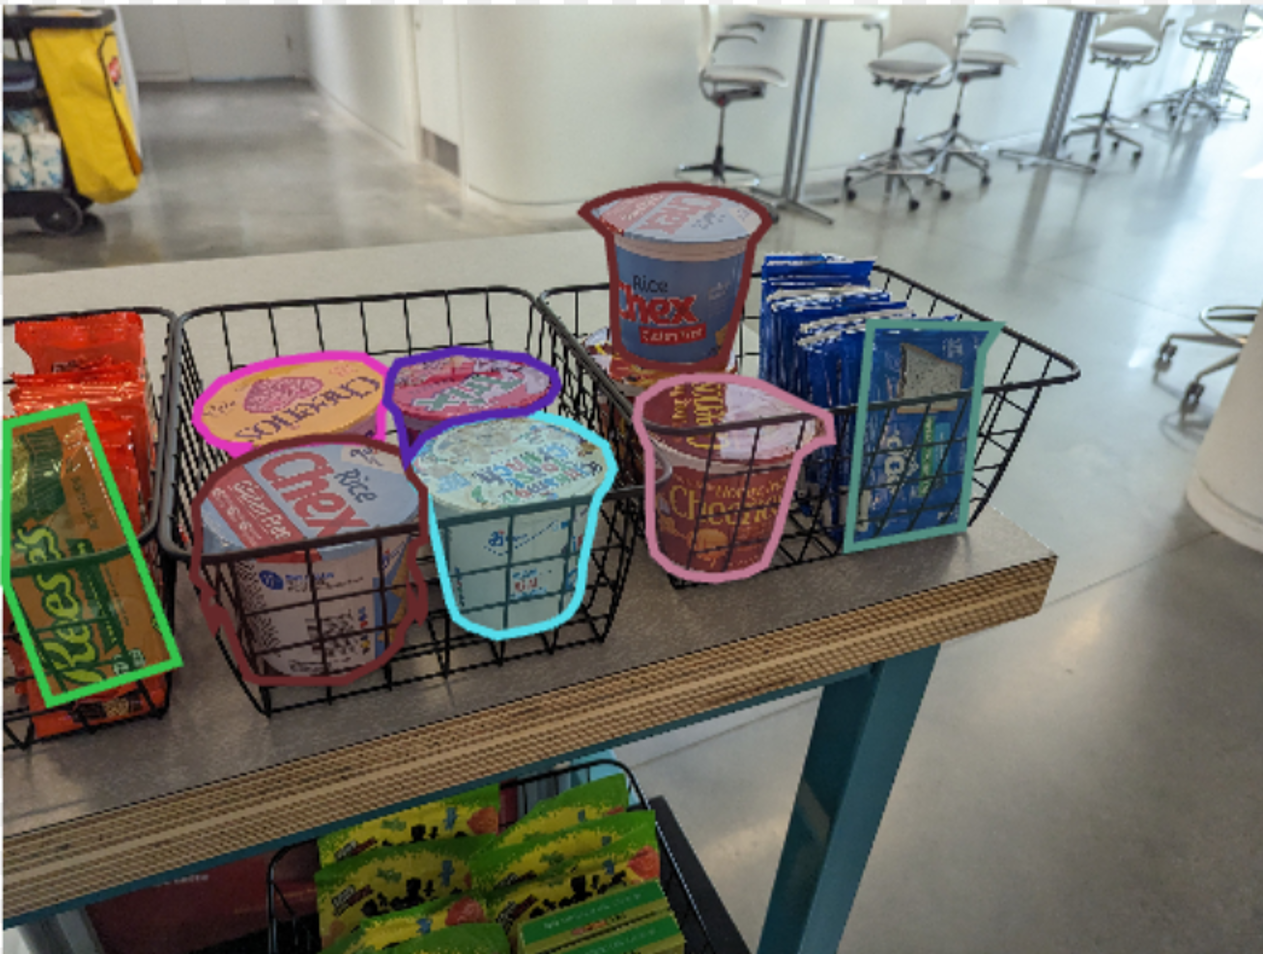
\includegraphics[width=0.5\linewidth]{Images/mask-data.png}
    \caption{Segmentation masks in Roboflow}
    \label{fig:seg-masks}
\end{figure}

\paragraph{Home}
The "Home" dataset was assembled with four classes and was primarily used during the development of the object detection system. The main location was a dresser in one author's room, on which up to four different food items were arranged. Annotations were produced using an "active learning" method with Label Studio. Active learning refers to an iterative process for automating data labelling, consisting of three steps:
\begin{enumerate}
    \item Data is labeled by humans
    \item A model is trained on that data
    \item The model is used to generate predictions for unlabeled data
    \item Humans fix the annotations with least certainty and repeat from step 2
\end{enumerate}
All annotations were bounding boxes, and care was taken to ensure that data was captured from multiple viewing angles. The class instance distribution was significantly more balanced compared to the Mosaic dataset, with more than 300 instances for each class. 

\paragraph{School Lab}
The "Lab" dataset was assembled with twelve classes, photographed  in the computer lab designated for testing. The limited number of classes lessened the amount of labelling necessary, and we were able to balance the class instances for this set as well. Annotations were produced with the active learning process in Label Studio. The \acrshort{yolo} model trained on this data performed well in similar testing environments to the lab, allowing us to conduct tests in other parts of the university to more efficiently engage testers.
\begin{figure}[h]
    \centering
    \begin{subfigure}[]{0.3\textwidth}
        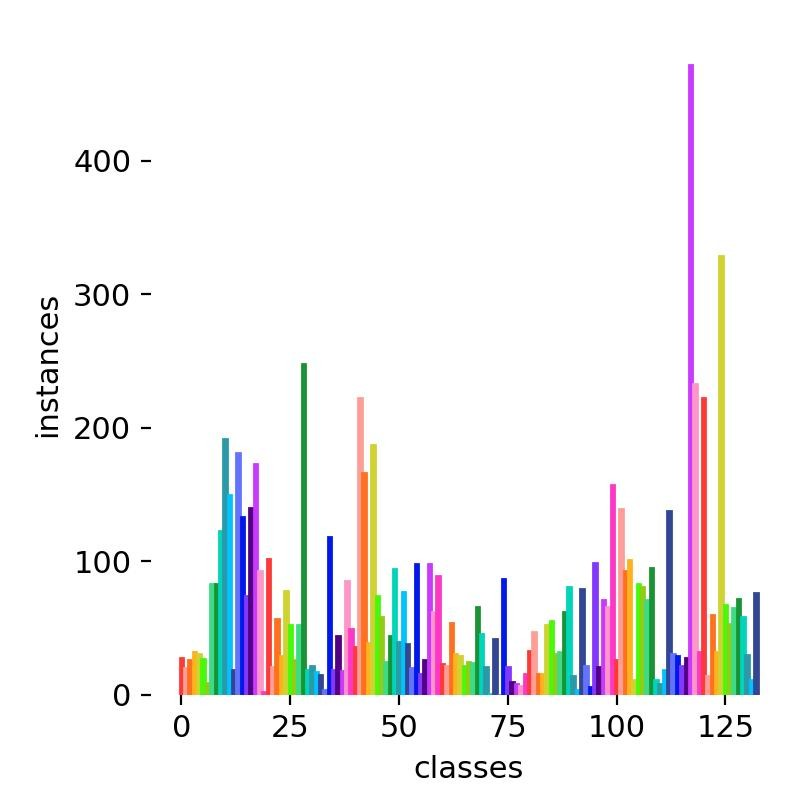
\includegraphics[width=\textwidth]{Images/mosaic-labels.jpg}
        \caption{Mosaic dataset}
        \label{fig:mosaic-dataset}
    \end{subfigure}
    \begin{subfigure}[]{0.3\textwidth}
        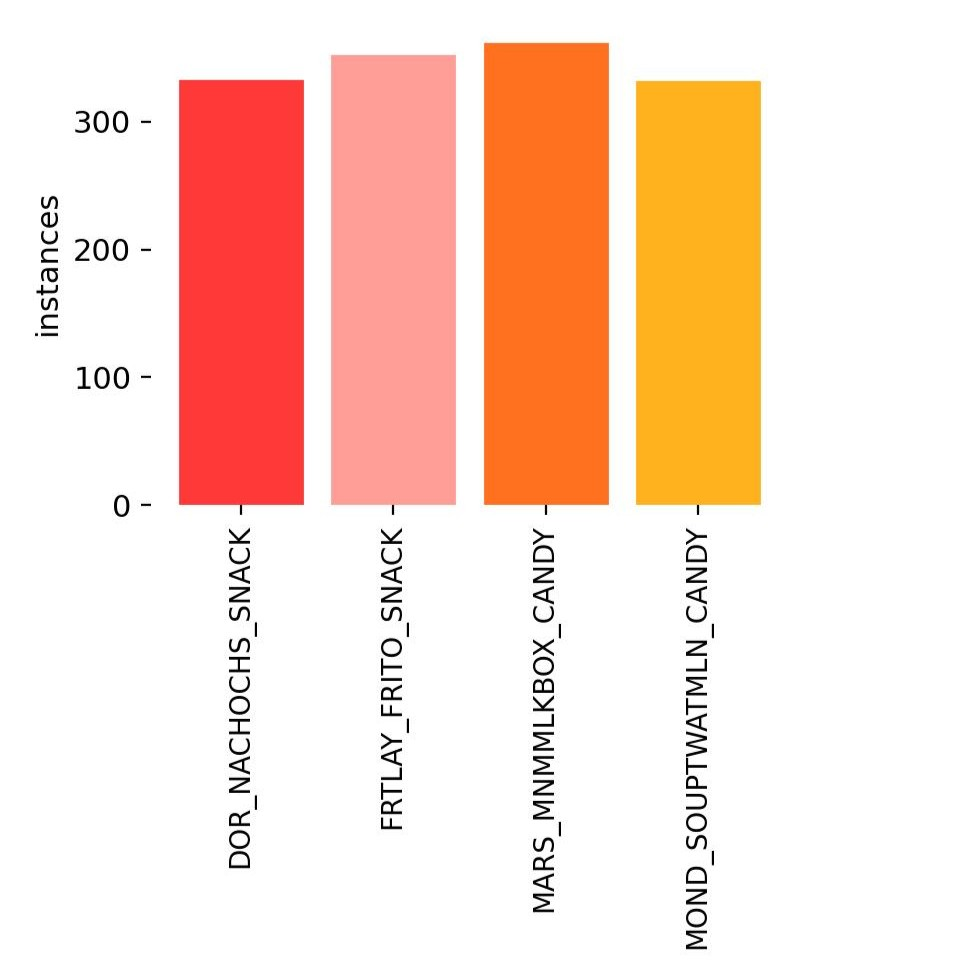
\includegraphics[width=\textwidth]{Images/roomset-labels.jpg}
        \caption{Home dataset}
        \label{fig:room-dataset}
    \end{subfigure}
    \begin{subfigure}[]{0.3\textwidth}
        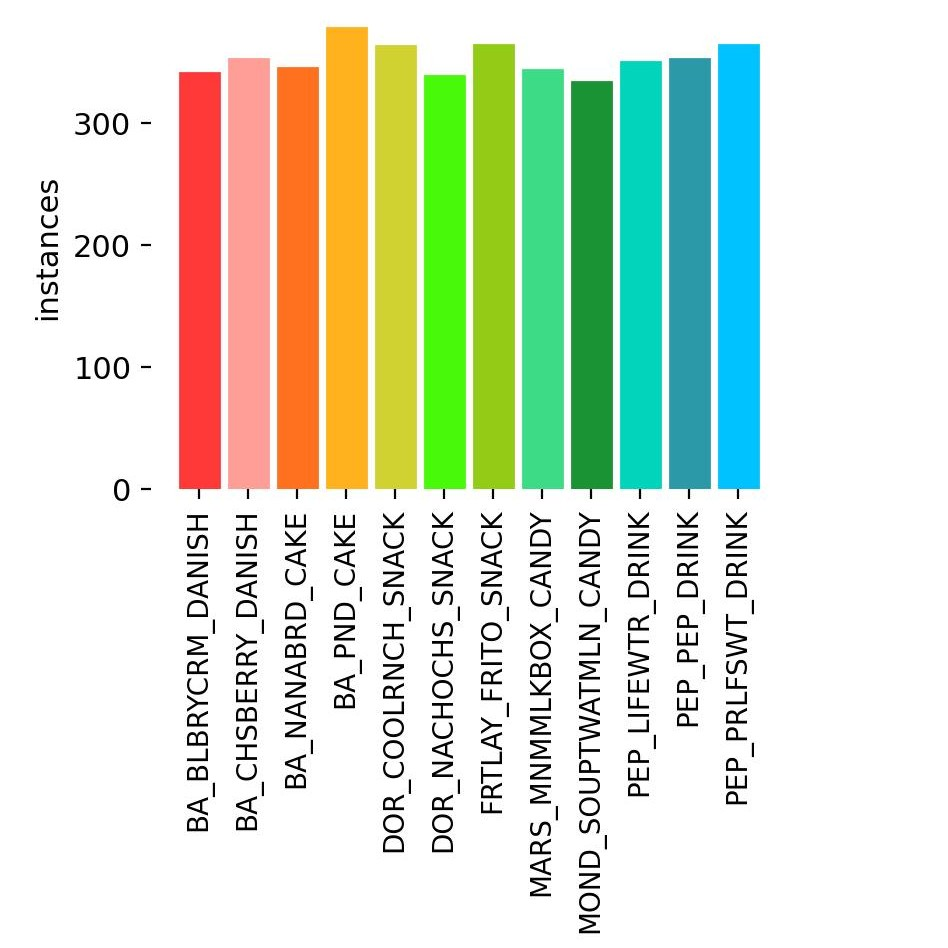
\includegraphics[width=\textwidth]{Images/labset-labels.jpg}
        \caption{Lab dataset}
        \label{fig:lab-dataset}
    \end{subfigure}
    \caption{Model class instance distribution graphs}
    \label{fig:dataset-labels}
\end{figure}


\begin{figure}[h!]
    \centering
    \begin{subfigure}[]{.65\textwidth}
        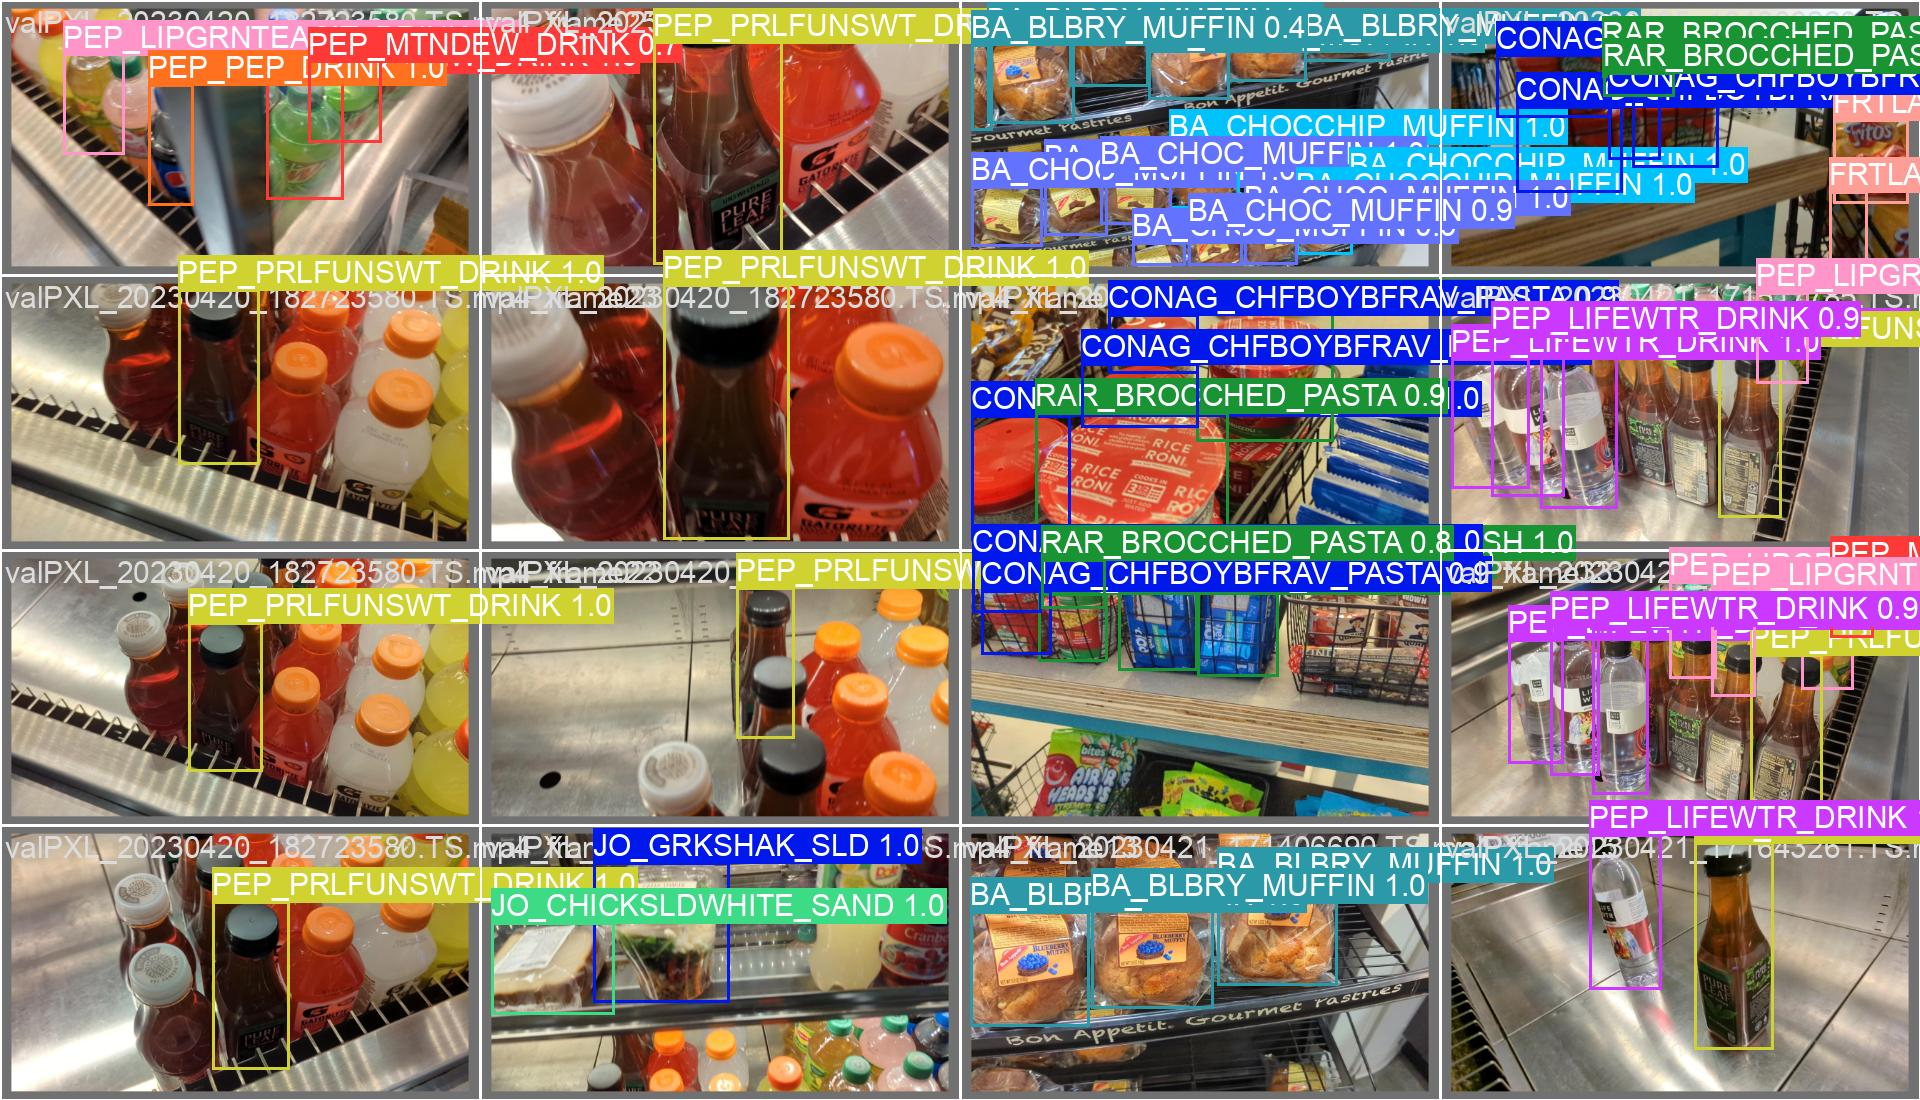
\includegraphics[width=\textwidth]{Images/mosaic-val.jpg}
        \caption{Mosaic dataset}
        \label{fig:mosaic-val}
    \end{subfigure}
    \begin{subfigure}[]{.65\textwidth}
        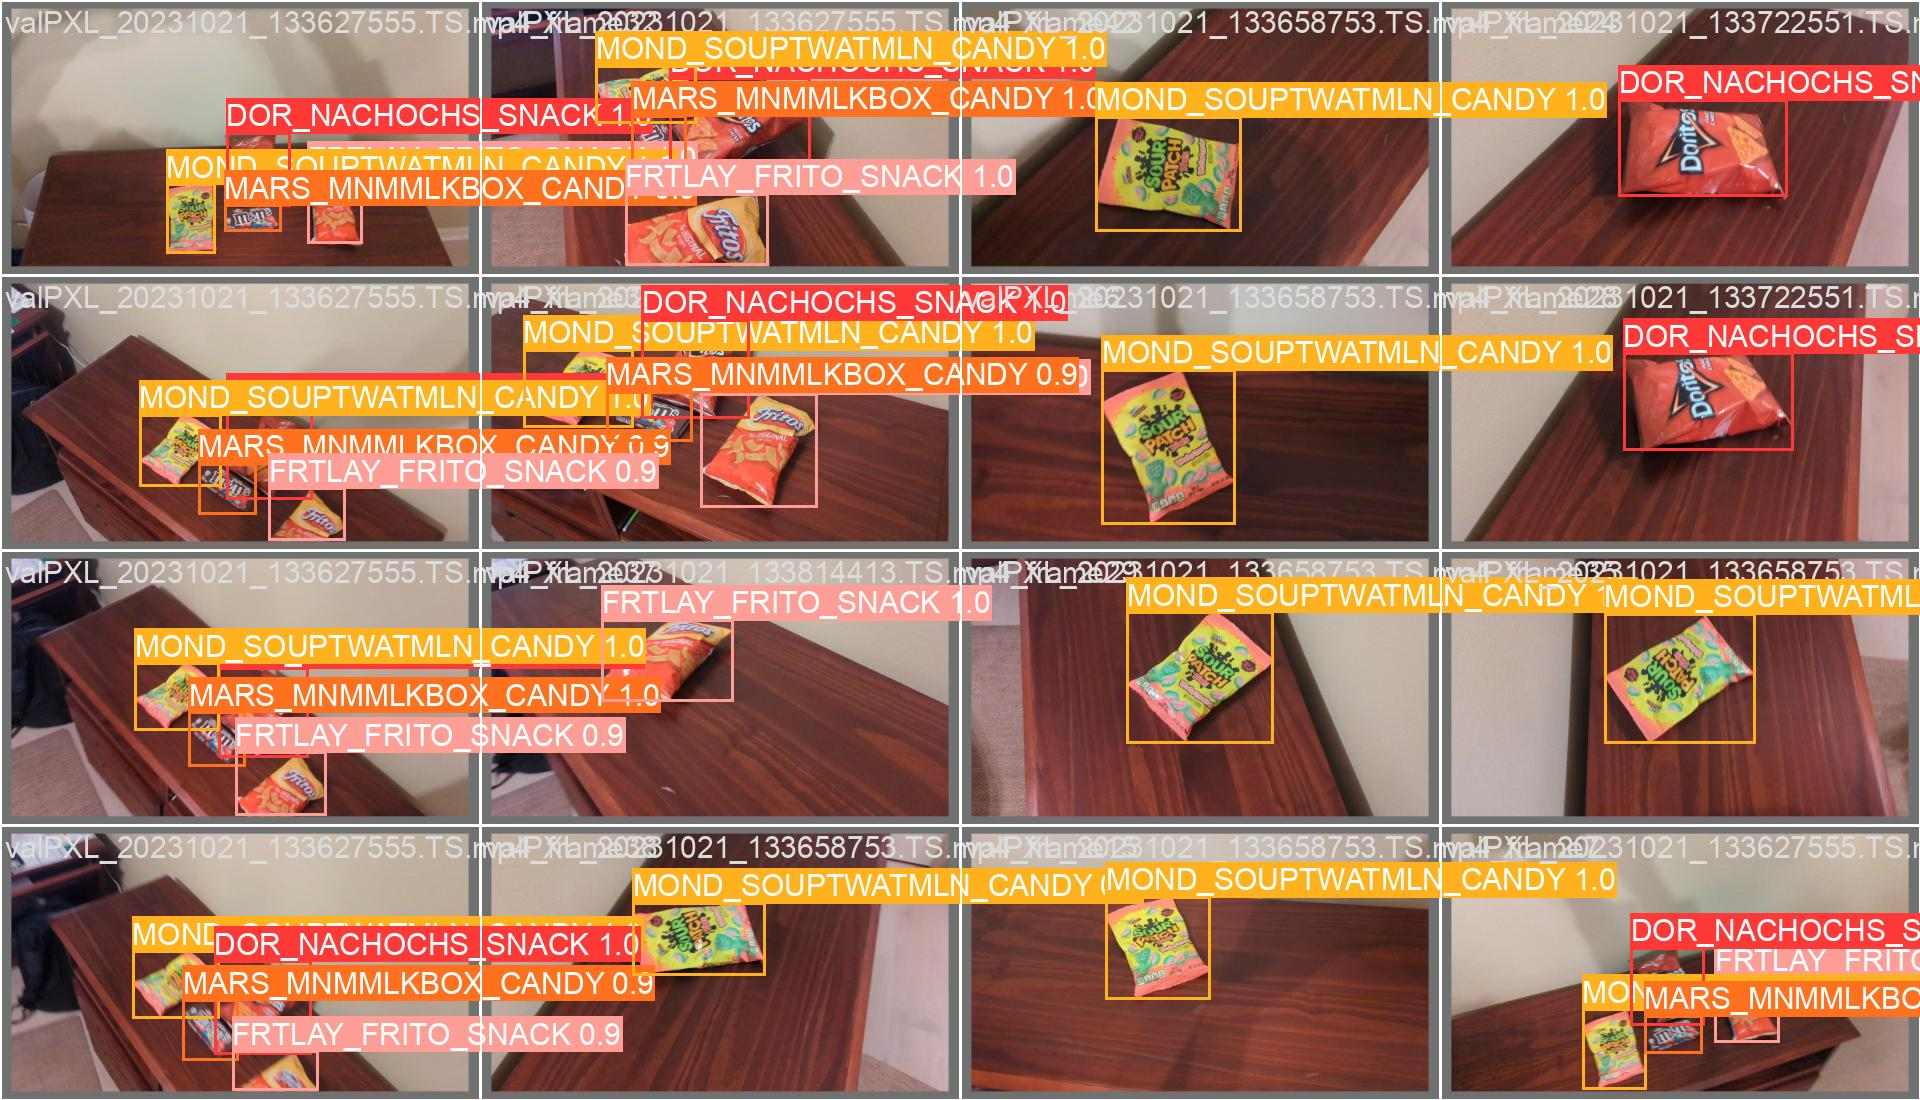
\includegraphics[width=\textwidth]{Images/roomset-val.jpg}
        \caption{Home dataset}
        \label{fig:roomset-val}
    \end{subfigure}
    \begin{subfigure}[]{.65\textwidth}
        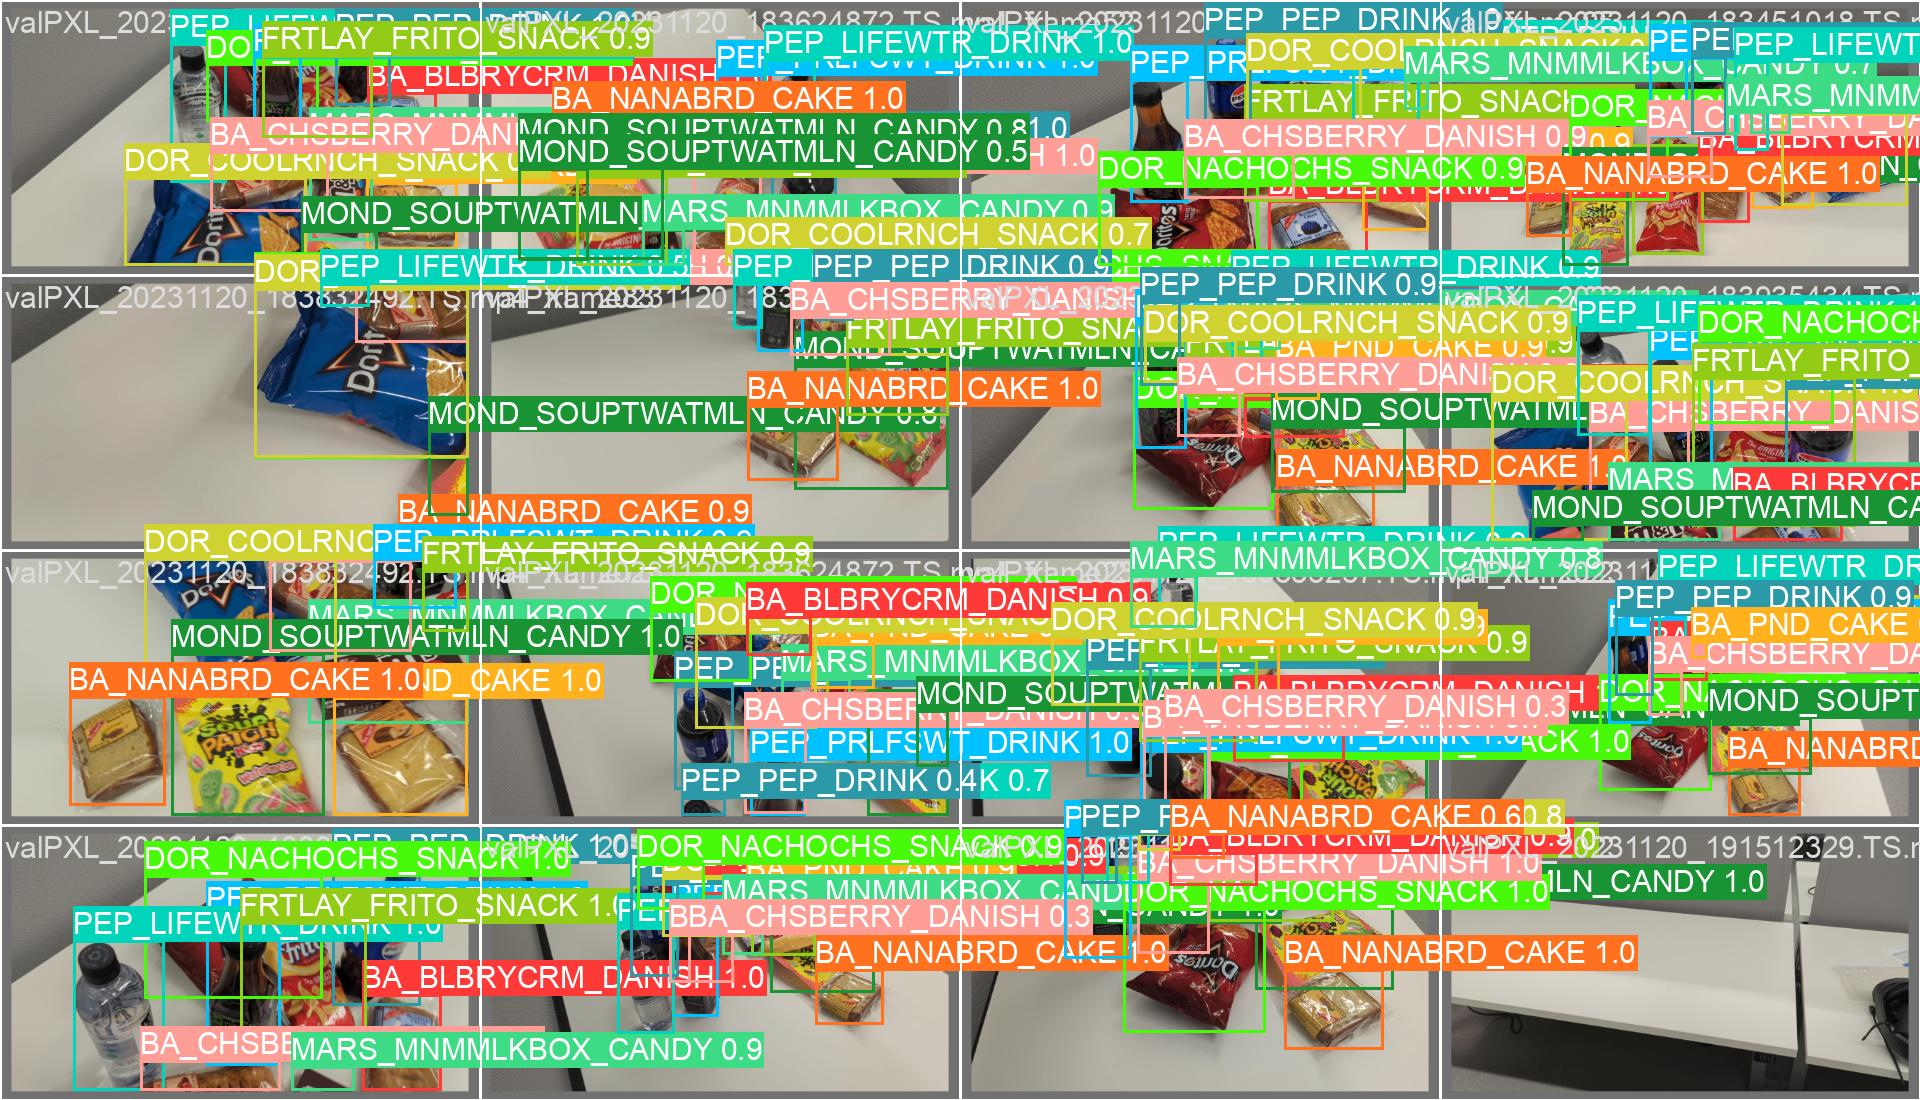
\includegraphics[width=\textwidth]{Images/labset-val.jpg}
        \caption{Lab dataset}
        \label{fig:labset-val}
    \end{subfigure}
    \caption{Model training validation samples}
    \label{fig:model-val}
\end{figure}
\paragraph{Model Training}
Active learning is a method for labelling and training on data in an iterative process. Label Studio\cite{LabelStudio} is an open-source software for annotating data, and allows for integration with custom training and prediction scripts. We developed a script that to generate predictions for the images we had, and to train on the completed annotations. We then would generate predictions, correct the generated bounding boxes with the lowest confidence, and then retrain the model on the newly annotated images. Correcting the predictions made by our model required significantly less time than manually adding all the boxes, and there was noticeable improvement in the model from run to run. We ran the training method every 50-100 images, for the recommended 100 epochs each time. We stopped annotating data once the model reached acceptable levels of confidence scores during training and predictions generated for labelling had minimal false positives and negatives. Figure \ref{fig:model-val} contains validation images from the training process for all three models.

\subsubsection{Database}
\paragraph{Structure}
Neo4j databases consist of nodes and relationships. There are no formal tables or need for foreign keys, allowing for easily searching many-to-many relationships based on a range of options. The main node type is "Item", representing the food or beverage. Items are connected to nodes representing the different nutritional data types, ingredients, and item tags. Ingredients can also be connected to sub-ingredients. Table \ref{tab:neo4jdb} describes the different nodes and relationships, and the values they contain.
\begin{table*}[h]\centering
\ra{1.2}
\caption{Neo4j database nodes and relations}\label{tab:neo4jdb}
\resizebox{\textwidth}{!}{%
    \begin{tabular}{@{}lllll@{}}
        \toprule 
        \textbf{Node Type} & \textbf{Properties} & \textbf{Relations} & \textbf{Properties} & \textbf{End Node} \\ \midrule
            &   & CONTAINS\_ALLERGEN     &  & Allergen   \\
            &   & MAY\_CONTAIN\_ALLERGEN &  & Allergen   \\ 
            &   & CONTAINS\_INGREDIENT   &  & Ingredient \\ %\cmidrule{3-5} 
            &   & CONTAINS\_NUTRIENT     & \begin{tabular}[c]{@{}l@{}}Amount, \\ (Percentage)\end{tabular} & Nutrient   \\ %\cmidrule{3-5}
            \multirow{-5}{*}[10pt]{Item} &  \multirow{-5}{*}[10pt]{\begin{tabular}[c]{@{}l@{}}class\_code, \\ name, \\ brand, \\ servings, \\ ingredient\_list\end{tabular}} & TAGGED\_AS &      & Item\_Tag \\ \cmidrule{1-5}
                Ingredient & name & CONTAINS\_SUBINGREDIENT &      & Ingredient \\
        \bottomrule
    \end{tabular}%
}
\end{table*}

\paragraph{Data Preparation and Import}
There was no prior database or centralized spreadsheet of nutritional information for the products sold at the Mosaic Cafe. Ingredient lists and nutritional data were compiled from photos of the product labels and cross referenced with data from SmartLabel. The products from Jack \& Olive had the least consistent labels, with multiple errors or missing/unlisted ingredients. Items were manually tagged with a range of categories based on dietary restrictions and food type or flavor to allow for easier search queries. 
\begin{figure}[h]
    \centering
    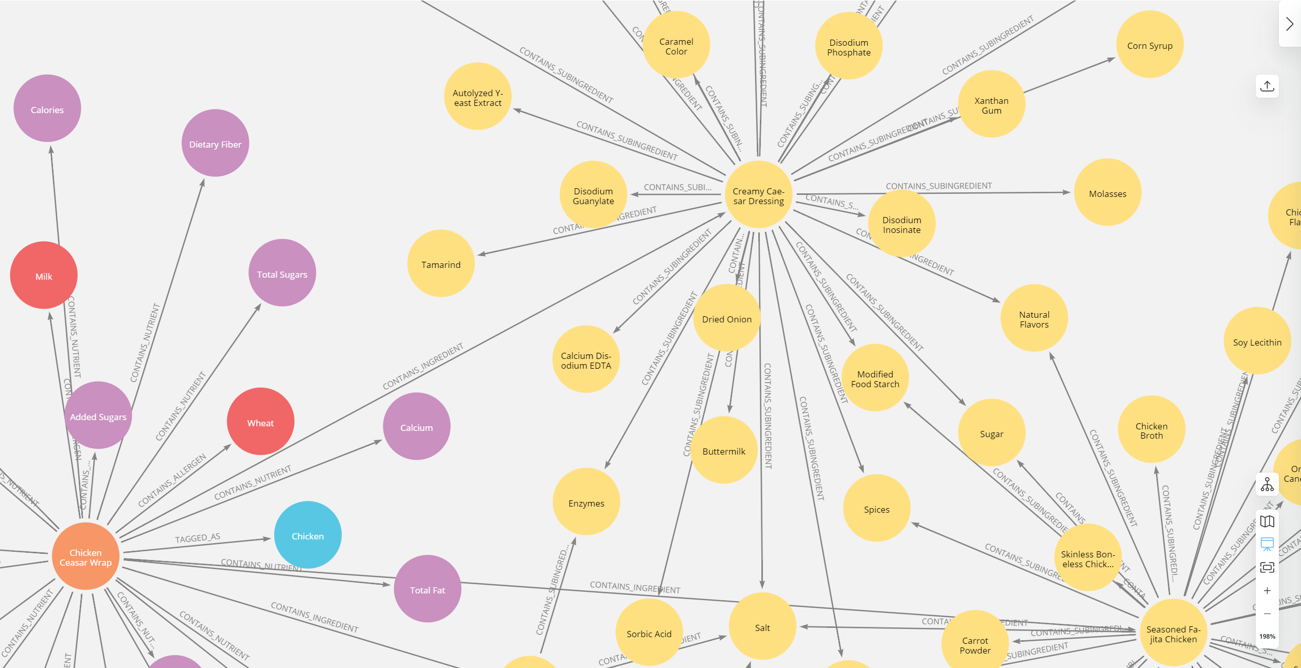
\includegraphics[width=\textwidth]{Images/neo4j.png}
    \caption{Partial view of an Item from our Neo4J database}
    \label{fig:neo4jnodes}
\end{figure}
Allergens were cross referenced between different items to be as accurate as possible, with separate columns in the spreadsheet for known and possible allergens. Caffeine content was included as a nutrient value and as a tag.

Neo4j allows the import of \acrfull{csv} data to create the nodes and relationships for the DB, via a custom script in Cypher, Neo4j's query language. There are three main tabs of the google sheet dedicated to the import data: ItemSchema, IngredientSchema, and AdditivesSchema. Many ingredient lists have ingredients with sub-ingredients. These are listed in the IngredientSchema page, while the full list as printed on the label (with corrections) is stored in the ItemSchema page. The additives page contains the various vitamins, sweeteners, and preservatives in columns by type. The import script can be found in the appendix.

\paragraph{Search Queries}
The item \verb|class_code| is used as the main identifier for items in both the object detector and the database. The code is abbreviated and contains the brand, item name, and item type to allow for identification at a glance. We used JavaScript on the client to dynamically generate the data for the search queries. In a true production environment, this is a safety risk, as the queries can be edited on the client side by malevolent actors; a better method would be to write the queries statically and pass the relevant data to the \acrshort{db}, but we chose this method for simplicity. All the data for the drop-down menus was queried on load and stored in the component state, while item information for the virtual augmentation was queried on marker load. 
The search query for parameters allowed and denied by the users was the most complex, requiring multiple attempts before settling on the final version shown below:
\begin{lstlisting}[language=Cypher]
OPTIONAL MATCH (a:Allergen|Ingredient|ItemTag WHERE a.name IN [${allowed}])
OPTIONAL MATCH (d:Allergen|Ingredient|ItemTag WHERE d.name IN [${denied}])
WITH collect(a) AS allowed, collect(d) as denied
MATCH (items:Item) WHERE ALL(a IN allowed WHERE (items)--(a) OR (items)--()-[:CONTAINS_SUBINGREDIENT]->(a)) 
MATCH (items:Item) WHERE NONE(d IN denied WHERE (items)--(d) OR (items)--()-[:CONTAINS_SUBINGREDIENT]->(d))
RETURN items.class_code AS class_codes
\end{lstlisting}

\paragraph{Deployment}
The production version of the database was limited to the twelve items in the final experiments. This was done to ensure users could only see items relevant to the testing. The Neo4j community edition server was deployed on the same \acrfull{aws} ECS instance as the web app for convenience; connecting over localhost was insufficient due to security requirements. WebXR requires secured \acrfull{tls} connections in all cases, requiring us to configure and deploy everything with certificates, including NginX and Neo4j. The Neo4j documentation does not make clear that the \acrshort{db} defaults to listening on IPv6. This will be important to account for in future work. 

\subsubsection{Object Detector}
\paragraph{WebXR Camera Access}
Raw Camera Access is the formal name for the feature of the WebXR \acrshort{api} that allows for pose-synchronized, real-time access to a mobile device's camera. This feature was formally implemented in Google Chrome in December of 2022. Previously, the only option for camera access was \verb|getUserMedia()|, providing access to camera images, but not synchronized with the virtual camera. For safety reasons, this prevented the calculation of camera intrinsics or accurate positioning. With the addition of the \verb|raw-camera-access| \acrshort{api}, we were able to directly access the camera texture, along with the data necessary to calculate the position of the user's device at that time. 

ThreeJS (and related libraries) was the 3d engine we used for the virtual augmentations and WebXR \acrshort{api} abstractions. At the time of development, ThreeJS's WebGL rendering loop had a direct incompatibility with the WebXR \verb|raw-camera-access| API, requiring us to contact the developers of Three to find a solution. The method we developed with their guidance is provided in Appendix A. The prescribed solution required re-binding the texture buffer away from Three's renderer, extracting the pixels, then binding the buffer back to Three. This allowed us to access the camera rendering layer while still benefiting from Three's model and interaction systems. 

A major issue we encountered during the development process involved a mismatch between the camera viewport and the screen size, leading to a large black border on two sides of the camera texture. The viewport and the screen have the same aspect ratio, allowing for ease of conversion for image coordinates, but ideally it should be possible to write directly to a buffer matching the viewport size without image corruption. Initially, this led to a consistent offset in the object detection results, combined with a steep loss in image quality during image resizing process. Unfortunately, we were unaware of the cause until late into the second development phase. This issue was noticeable for participants during the first user test.  We solved the issue in time for the second user test by cropping the image to the viewport size instead of resizing the whole image.

\paragraph{Client/Server Networking}
The client and server communicate via a secure web-socket connection. WebXR requires all connections to and from the client to be encrypted with \acrshort{tls} to ensure user privacy. To simplify the network configuration and \acrshort{tls} connection, we used a reverse-proxy service (i.e., Ngrok) to connect the socket. This provided a simple connection from our \acrshort{aws} hosted client to the back-end server without needing to open ports on the network. 
Sending and receiving the image data required us to implement a WebWorker, JavaScript's solution for multi-threading. Without the worker, sending the frames would cause the app to freeze for a second or more every time data was sent. The worker handled cropping and resizing the frame to match the image size required by \acrshort{yolo} (640px), maintaining the socket connection and reconnecting, and sending and receiving the necessary metadata and responses to and from the server.

\paragraph{\acrshort{yolo} Image Analysis Back-end Server}
To lessen the amount of processing performed by the client device, we developed a remote server application to run the \acrshort{yolo} model. We used the FastAPI library for Python to handle the websocket connection request, and to process the additional class metadata. The system was implemented as a proof of concept, and would need to be heavily reworked to allow for multiple users. The current system stores information about the search classes on the server and reuses that information for every frame; a proper system would either utilize a proper database with \verb|userIDs|, or to receive the metadata with each frame. 

In the current implementation, the server utilizes a queue to hold incoming frames for processing. Additional frames beyond the queue are dropped until there is available space. The object detection model was fast enough that queue backlog was rarely an issue, but malformed frames or other incorrect data leads to permanent clogging, this should be addressed for a production setup. 
The backend also performs the structuring of the results into an easier form for use on the frontend. 

\paragraph{Real World Object Location}
WebXR creates objects referred to as "anchors" to represent tracked locations in the real world. Our system uses the coordinates returned from the \acrshort{yolo} model to determine where to place the anchors, and then attaches models to them. 

The process to determine a point's location in space consists of three steps:
\begin{enumerate}
    \item Adjust the coordinate system origin and create an \verb|XRHitTestSource| with an \verb|offsetRay| that matches the coordinates
    \item Perform a hit-test (raycast) from the source to the object
    \item Create an anchor from the first \verb|XRHitTestResults| returned from  \verb|getHitTestResults()|
\end{enumerate}
For much of the development process, we had constant issues with aligning the virtual markers to their physical counterparts. There were two causes: the size mismatch between the camera viewport and the texture buffer, and confusion over the coordinates for the offset ray. The coordinate option we chose for the \acrshort{yolo} prediction data was "normalized XYWH." Normalizing the values to be between 0 and 1 allowed us to easily set the offset, as the aspect ratios for the different views were the same. The coordinate system used for computer vision, including our \acrshort{ai} model, generally places the origin in the top left corner of the image. The device screen coordinate origin is centered, however, requiring conversion. The second point of confusion stemmed from inconsistency in the definition of "XYWH" box data. For our system, we needed the center of the bounding box. The standard definition for XYWH boxes is top-left origin (XY) plus the width and height. YOLO's bounding boxes are already formatted with "XY" at the center, but the documentation is not clear on this, which led us to incorrectly offset the anchors and markers from the screen origin. This impacted our testing during the first user study.  We solved the issues with the marker placement in time for the second study.
\filbreak
\paragraph{\acrshort{aws} Sagemaker Deployment}
In the few weeks before the second user study, we spent one week attempting to make the changes necessary to deploy our model to AWS Sagemaker, Amazon's machine learning deployment platform. We initially designed our system using web-sockets for the connection, based on their speed and ease of sending binary image data. Sagemaker utilizes HTTP and REST to provide computation endpoints that multiple users can connect to and receive model predictions from. This would have solved the production issues with the current FastAPI back-end server, allowing for a better user experience and the possibility of running multiple tests at the same time. There were several major factors that led to us rejecting Sagemaker as a possible solution, however:
\begin{enumerate}
    \item Cost - AWS charges based on usage, and Sagemaker requires the use of many additional services
    \item Complexity - Endpoints cannot store any data between operations, requiring major rewrites to the client and full rewrite of the model code
    \item Difficulty - Lack of documentation, useless error logs, and predatory design patterns
\end{enumerate}
After investing significant time in implementing the code required for Sagemaker, we decided multi-user functionality was not practically achievable within the scope of this project, and left it to future work. A breakdown of the AWS services used for the project deployment is in Table \ref{tab:sagemaker}.

\begin{table}[h]\centering
\caption{\acrshort{aws} Sagemaker endpoint hosting and deployment costs.}\label{tab:sagemaker}
\ra{1.2}
\resizebox{\textwidth}{!}{%
    \begin{tabular}{@{}llll@{}}
    \toprule
        \textbf{Service} &   \textbf{Purpose} &   \textbf{Cost}    &   \textbf{Notes}   \\ 
        \midrule
        Elastic Cloud Compute (EC2) &   Virtual Private Server  &   \$25    &   Server hosting for web app and database \\
        Route 53    &   Domain registration &   \$0.50  &   Domain name and records registration    \\
        Sagemaker   &   Machine Learning    &   \$50    &   Model endpoint deployment   \\
        Cloudwatch  &   Logging &   \$3 & Only way to view logs, errors cut off if response is too long \\
        API Gateway &   REST API    &   \$0.01  &   Allows outside access to Sagemaker Endpoint \\ 
        Simple Storage Service (S3) &   Cloud Storage   &   \$0.02  &   Stores model package, requires upload for every change    \\
        Lambda  &   Serverless Code &   &   Receives response from REST and calls the endpoint  \\
    \bottomrule
    \end{tabular}%
}
\end{table}
\subsubsection{User Interface}
The main goals for the user interface were to provide the user with information as clearly as possible, differentiate between options using color and shape for accessibility, and to maximize the space dedicated to the camera view. 

\paragraph{Landing Page}
Before users enter the \acrshort{ar} experience, they start at a landing page. This is required by the WebXR standard for user security to ensure the user has control of when the camera activates. Figure \ref{fig:landing-pages} compares the landing pages for the first and second versions of our application, and the differences in \acrshort{ui} for the web-app in the browser vs. installed as a \acrshort{pwa}.

\begin{figure}[h]
    \centering
    \begin{subfigure}[]{0.3\textwidth}
        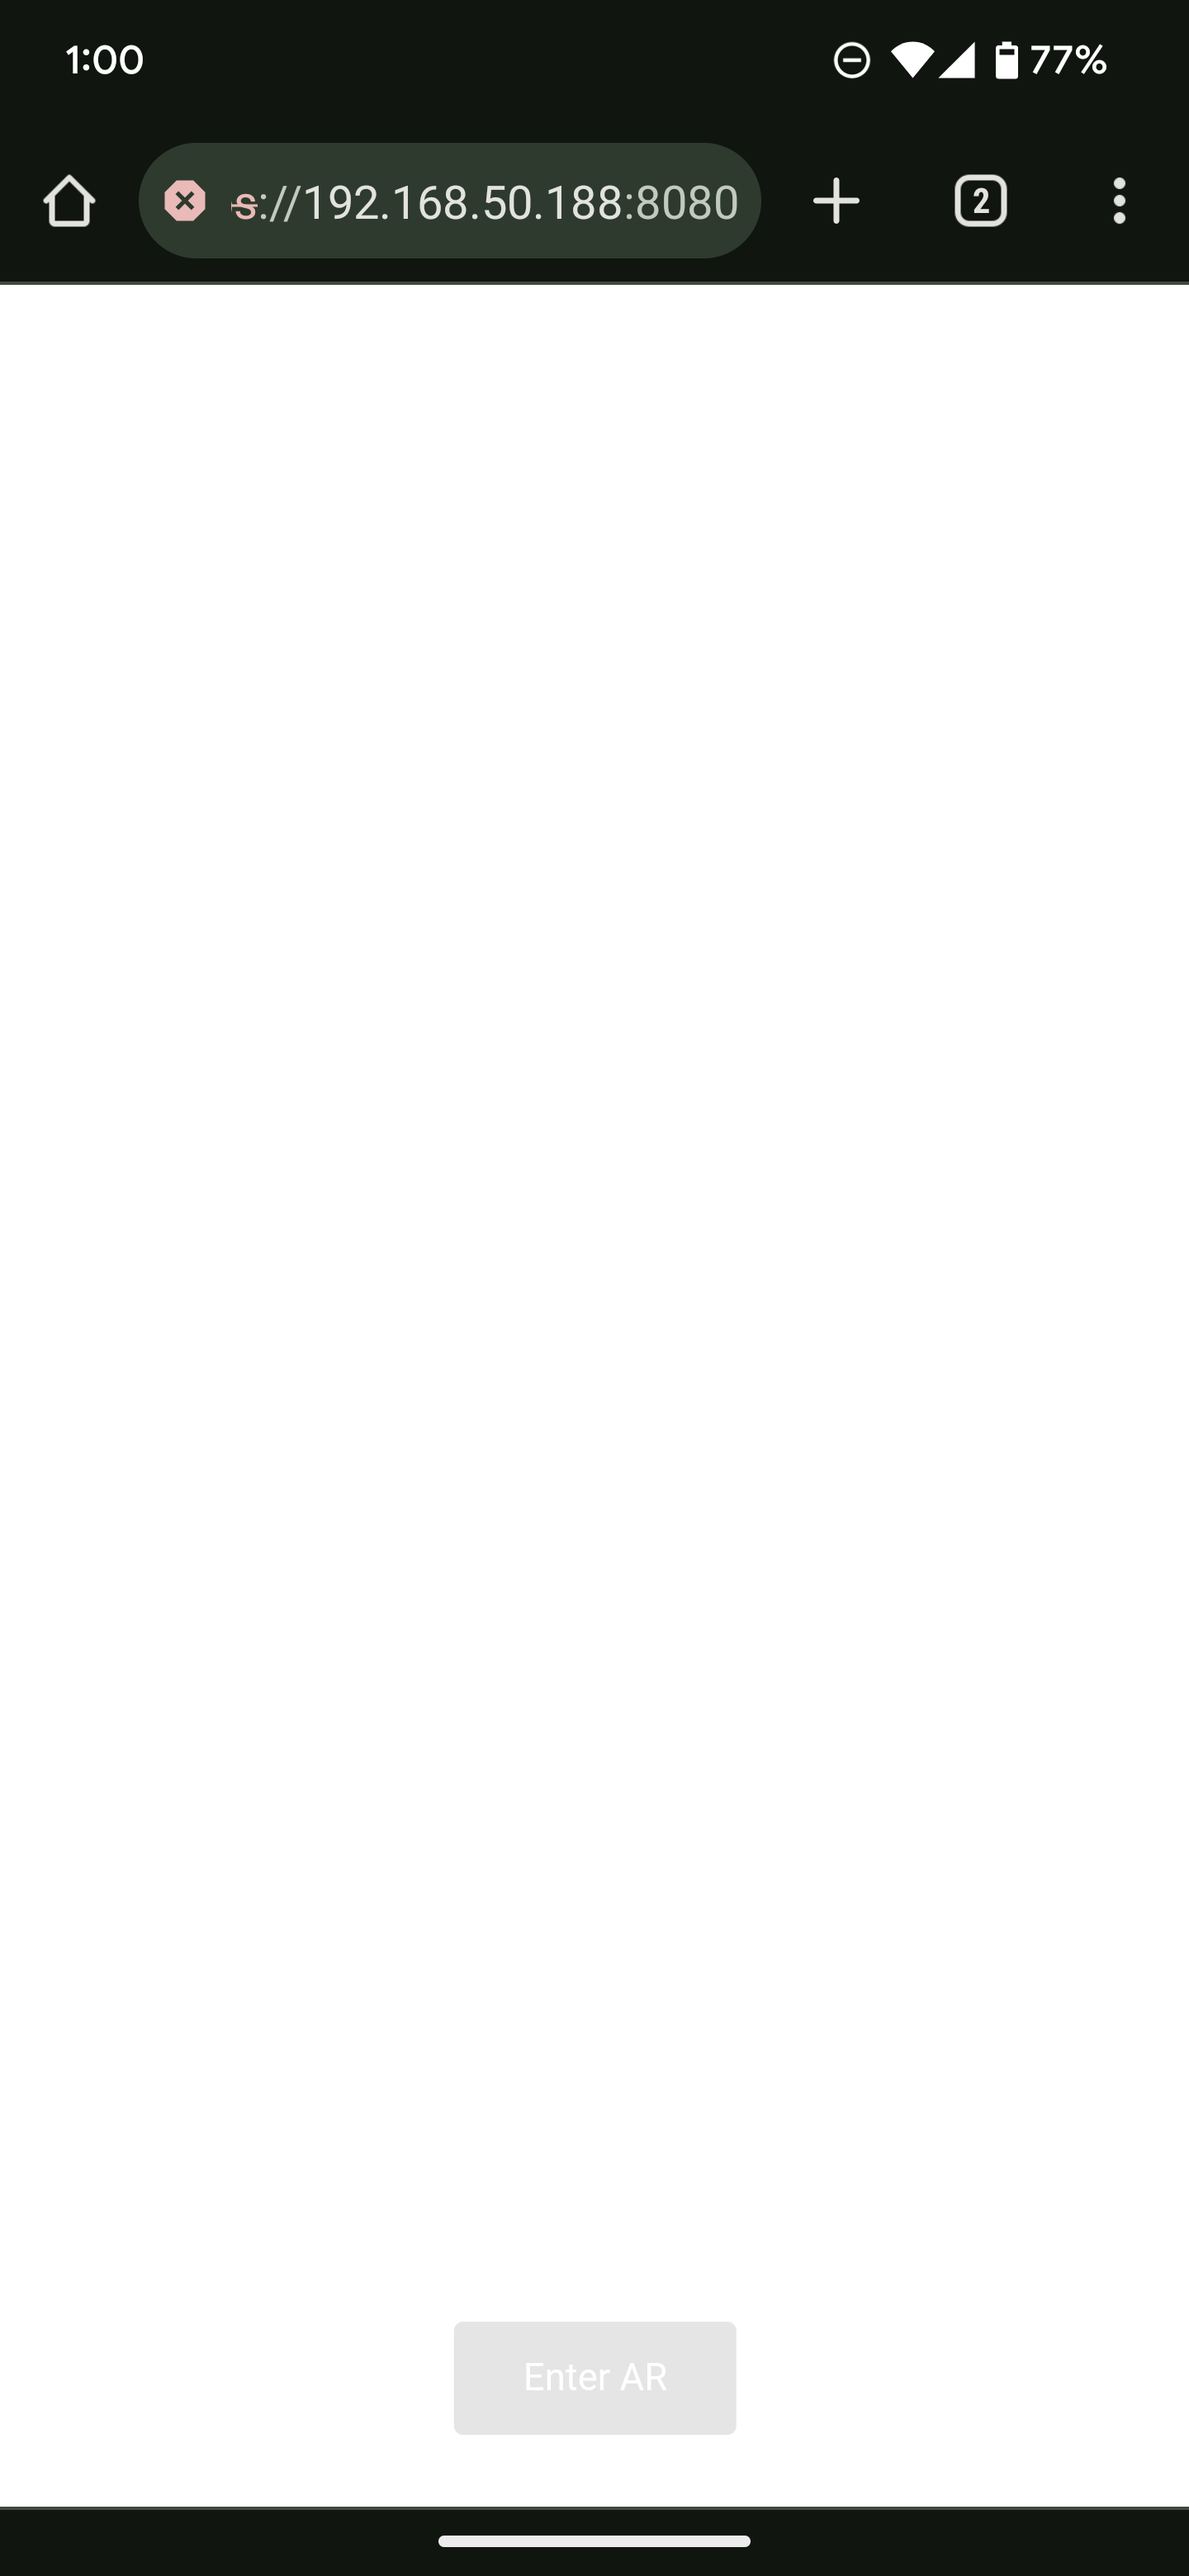
\includegraphics[width=\textwidth]{Images/mainmenuv1.png}
        \caption{Version 1}
        \label{fig:original}
    \end{subfigure}
    \begin{subfigure}[]{0.3\textwidth}
        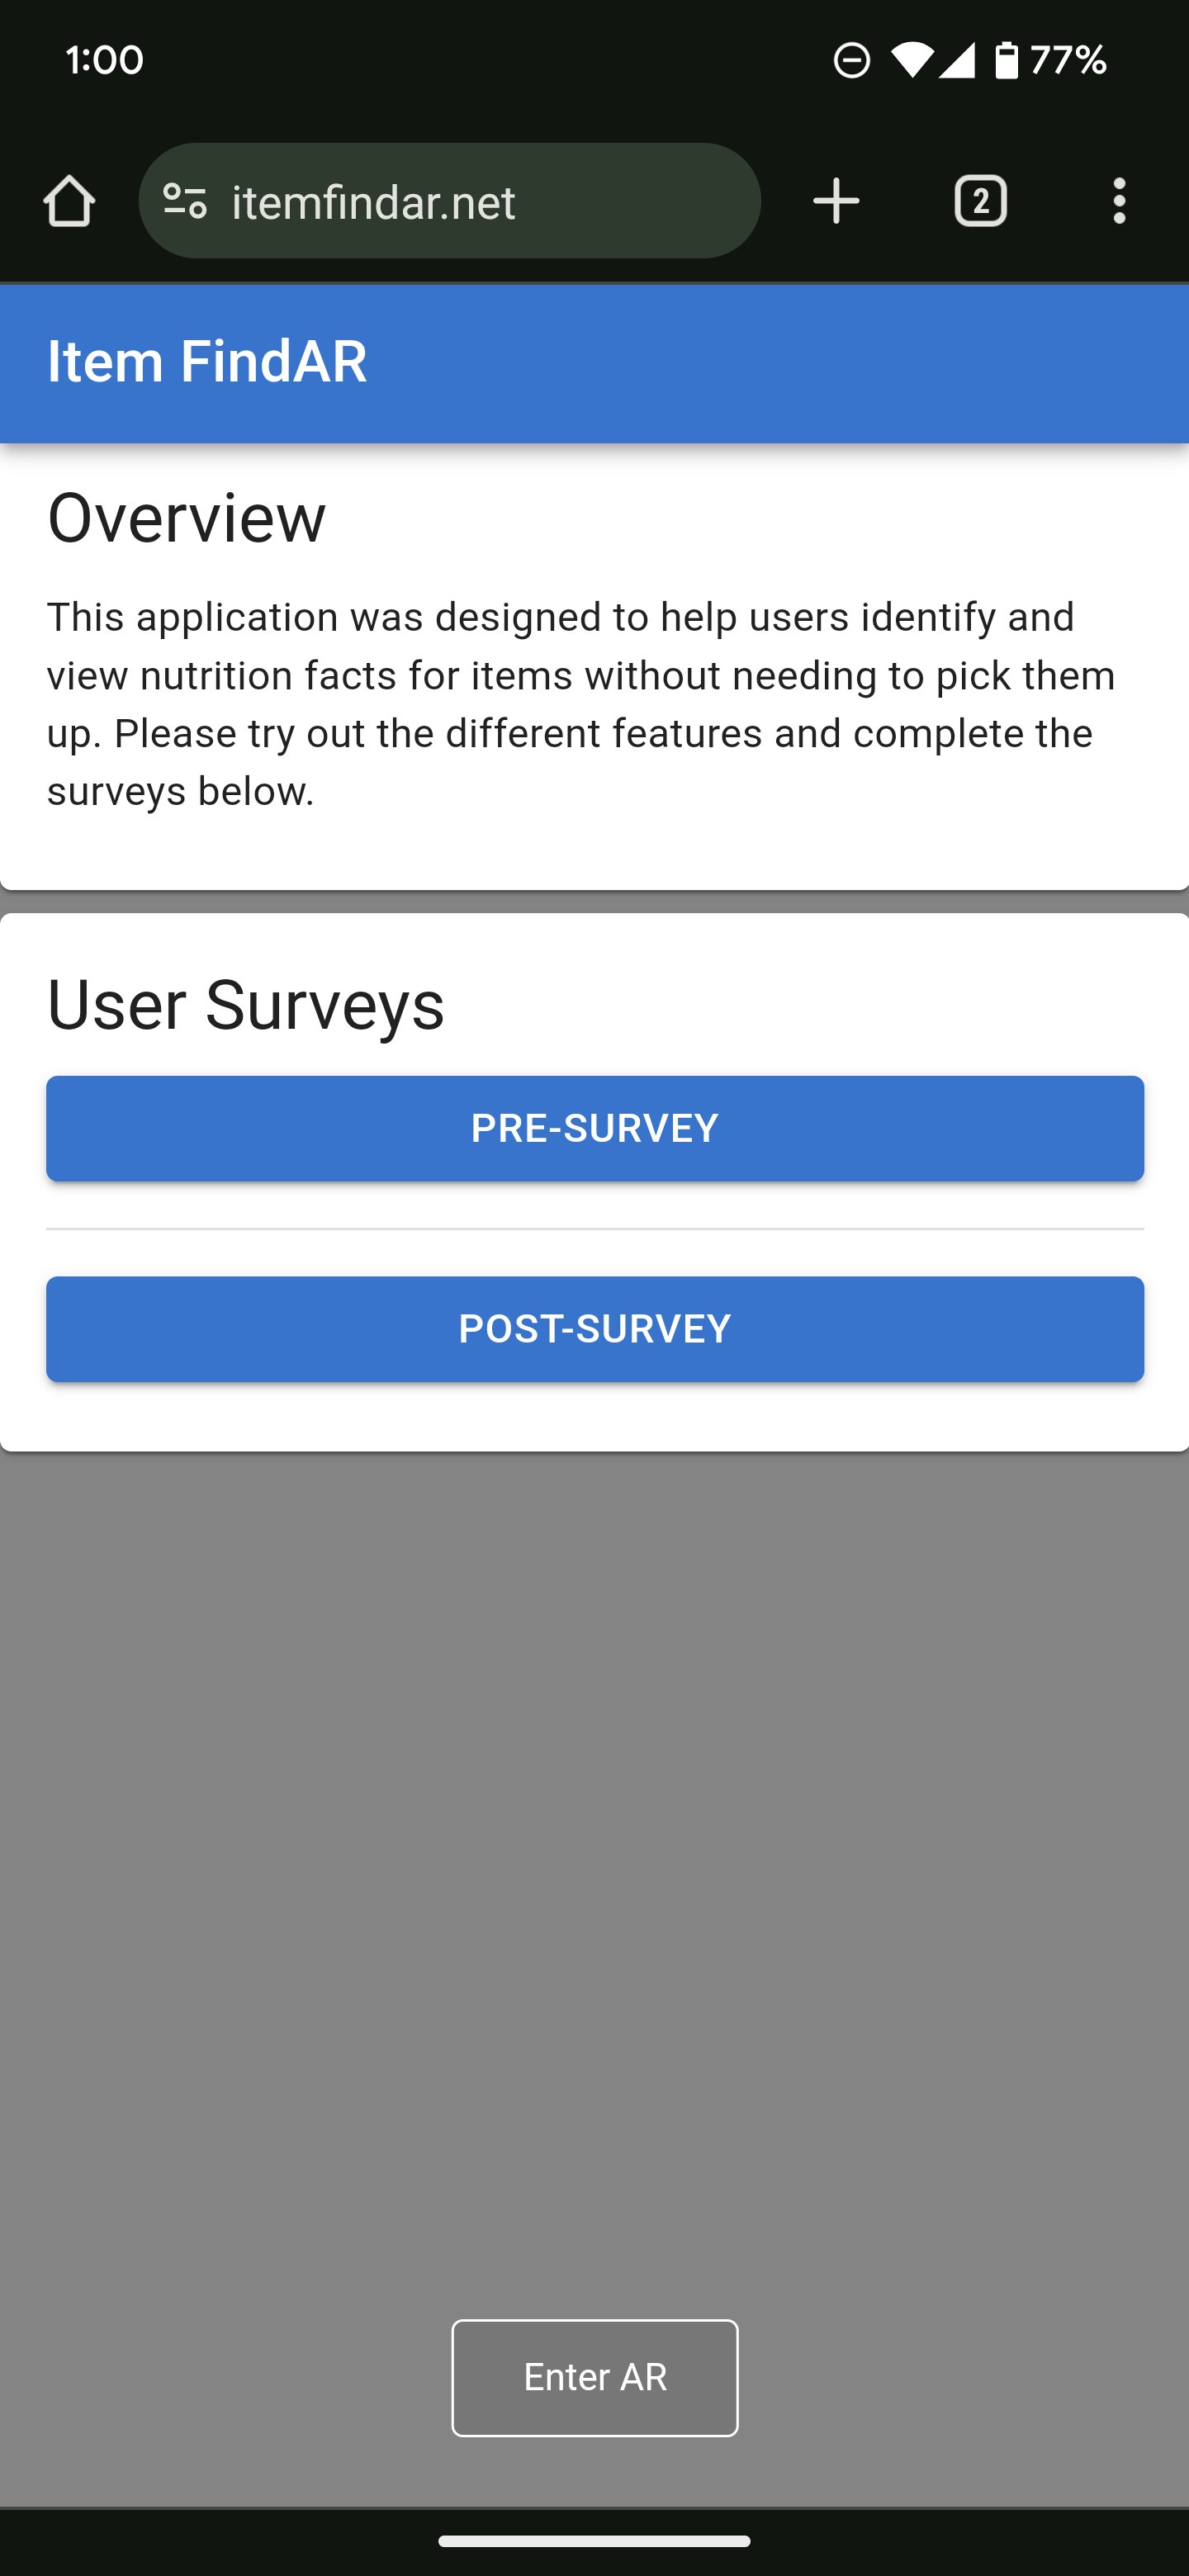
\includegraphics[width=\textwidth]{Images/mainmenuv2.png}
        \caption{Version 2}
        \label{fig:v2}
    \end{subfigure}
    \begin{subfigure}[]{0.3\textwidth}
        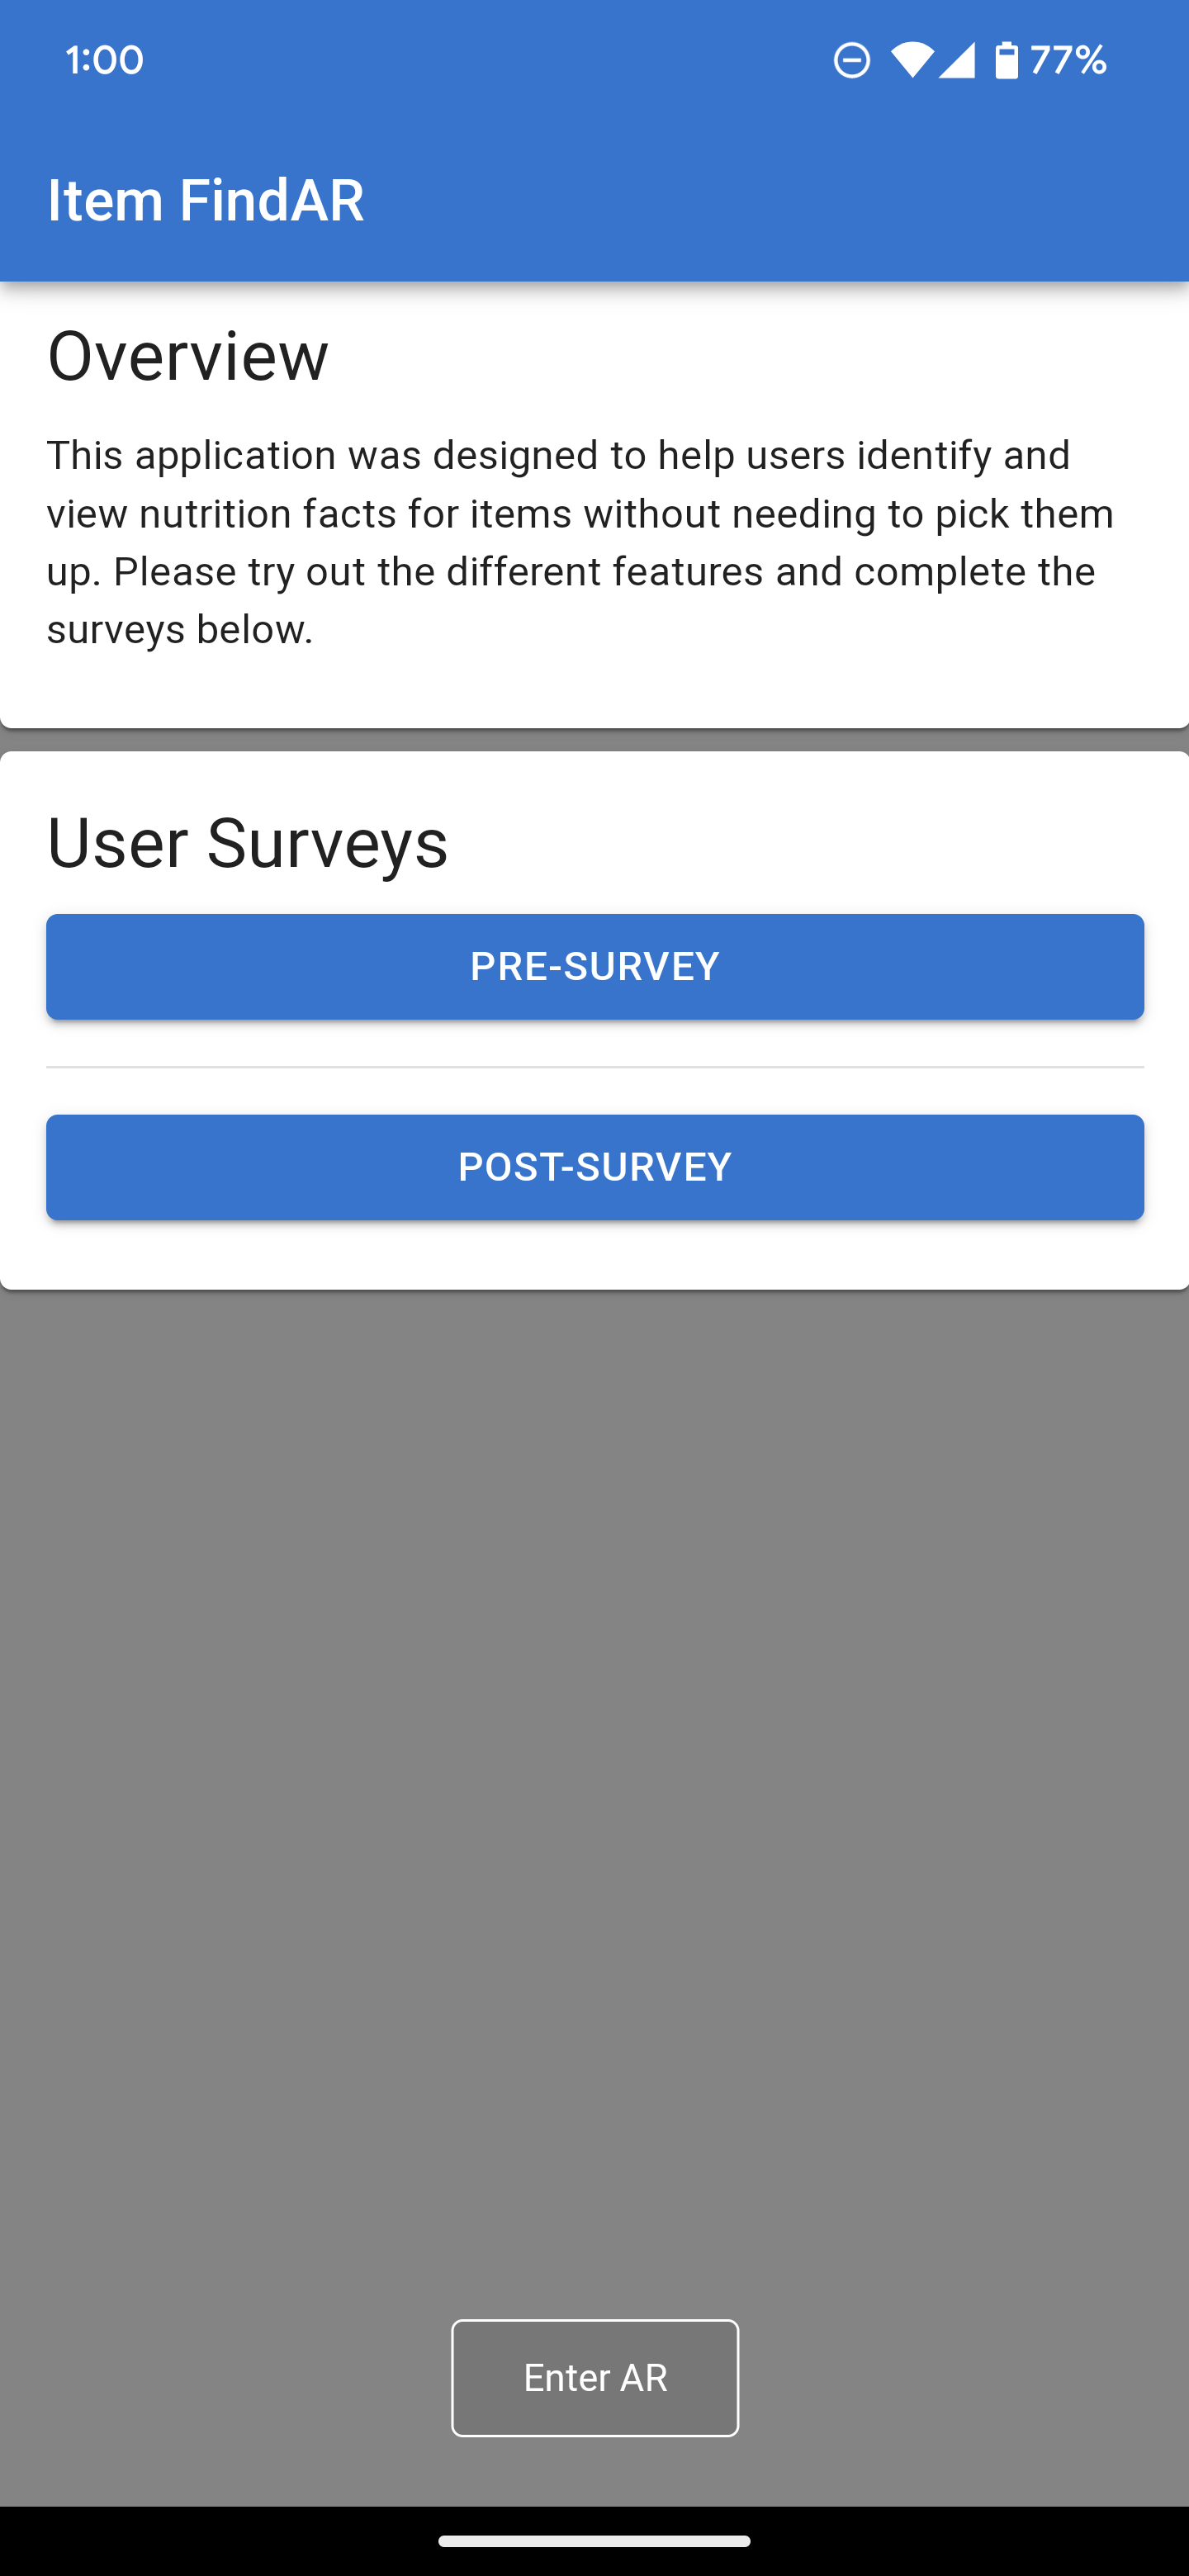
\includegraphics[width=\textwidth]{Images/pwav2.png}
        \caption{Version 2 PWA}
        \label{fig:v2-pwa}
    \end{subfigure}
    \caption{Landing page and \acrshort{ui} differences between versions}
    \label{fig:landing-pages}
\end{figure}
\filbreak
\paragraph{Virtual Augmentations}
There are two main parts to the augmented reality interface: 
\begin{enumerate}
    \item the \verb|ItemMarker| that marks item locations and displays warnings
    \item  the nutrition menu that displays the ingredients and nutrients and allergens.
\end{enumerate}
The \verb|ItemMarker| system attaches simple models to the item anchors, either a green checkmark, an orange alert symbol, a red warning marker, or a neutral circle, as shown in Figure \ref{fig:augment-ui}. We chose to use different shaped markers to make the system more accessible to users with color vision issues. Users can tap on the markers to select the item and open the nutrition menu, and tap it again to close the menu. We change the transparency of the selected item's marker to allow users a better view of the item and hide any other markers to avoid covering the nutrition menu. One major improvement would be to create a hidden object that users could tap on to make hitting the marker less difficult. %% ***ahamam*** add screenshots


\begin{figure}[h!]
    \centering
    \begin{subfigure}[]{0.3\textwidth}
        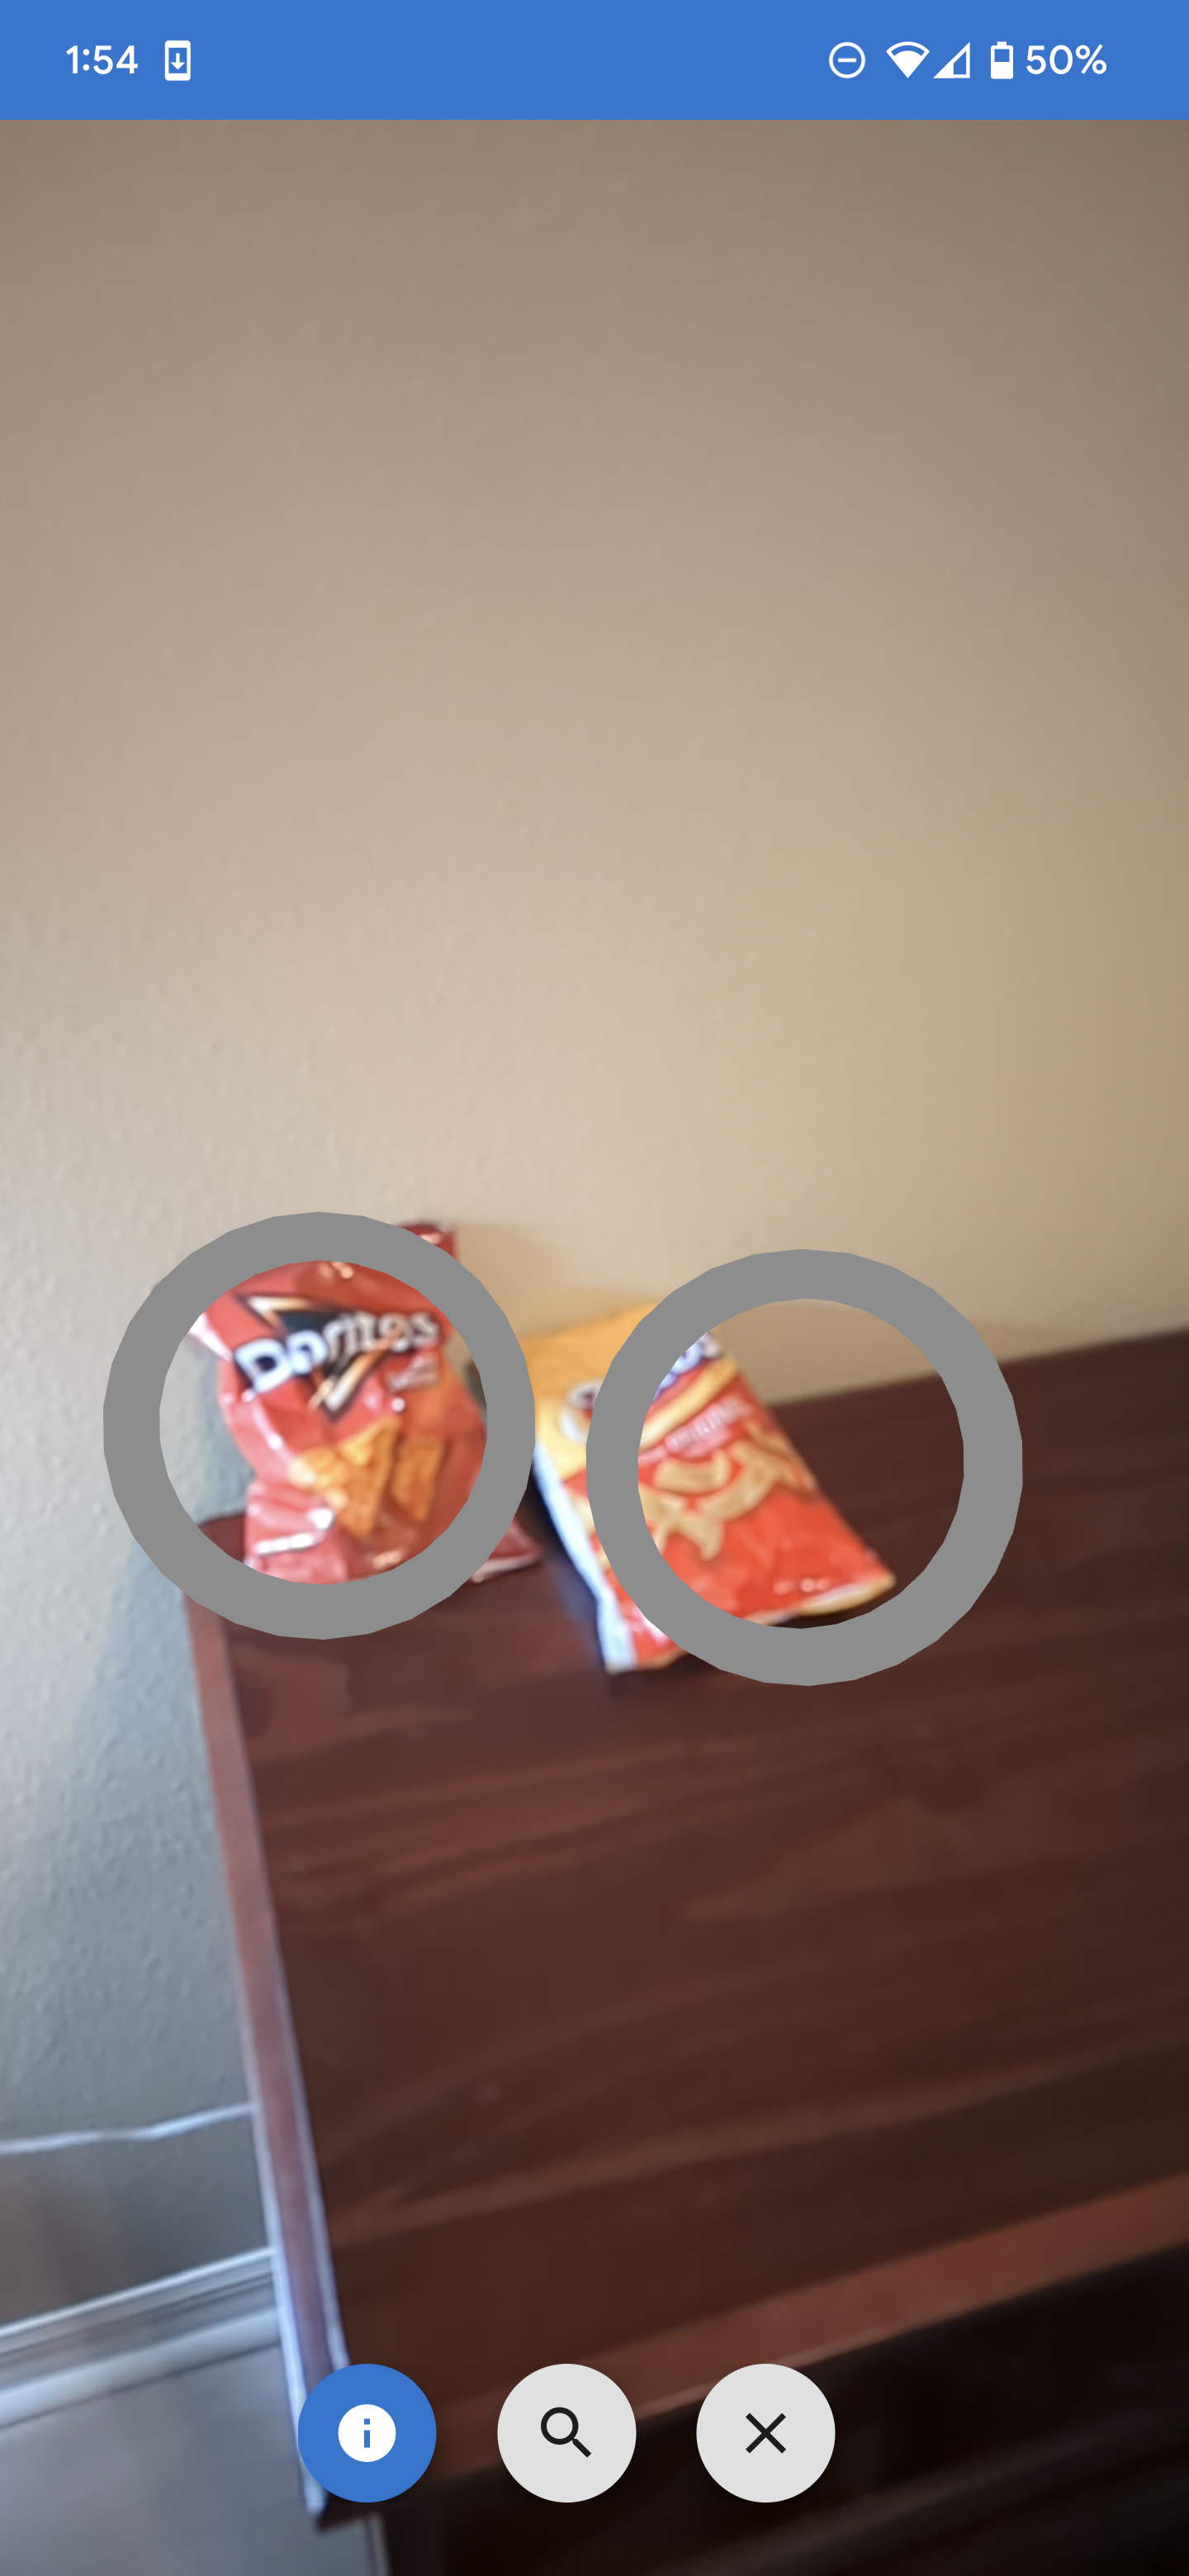
\includegraphics[width=\textwidth]{Images/neutral.png}
        \caption{Neutral markers}
        \label{fig:neutral-mark}
    \end{subfigure}
    \begin{subfigure}[]{0.3\textwidth}
        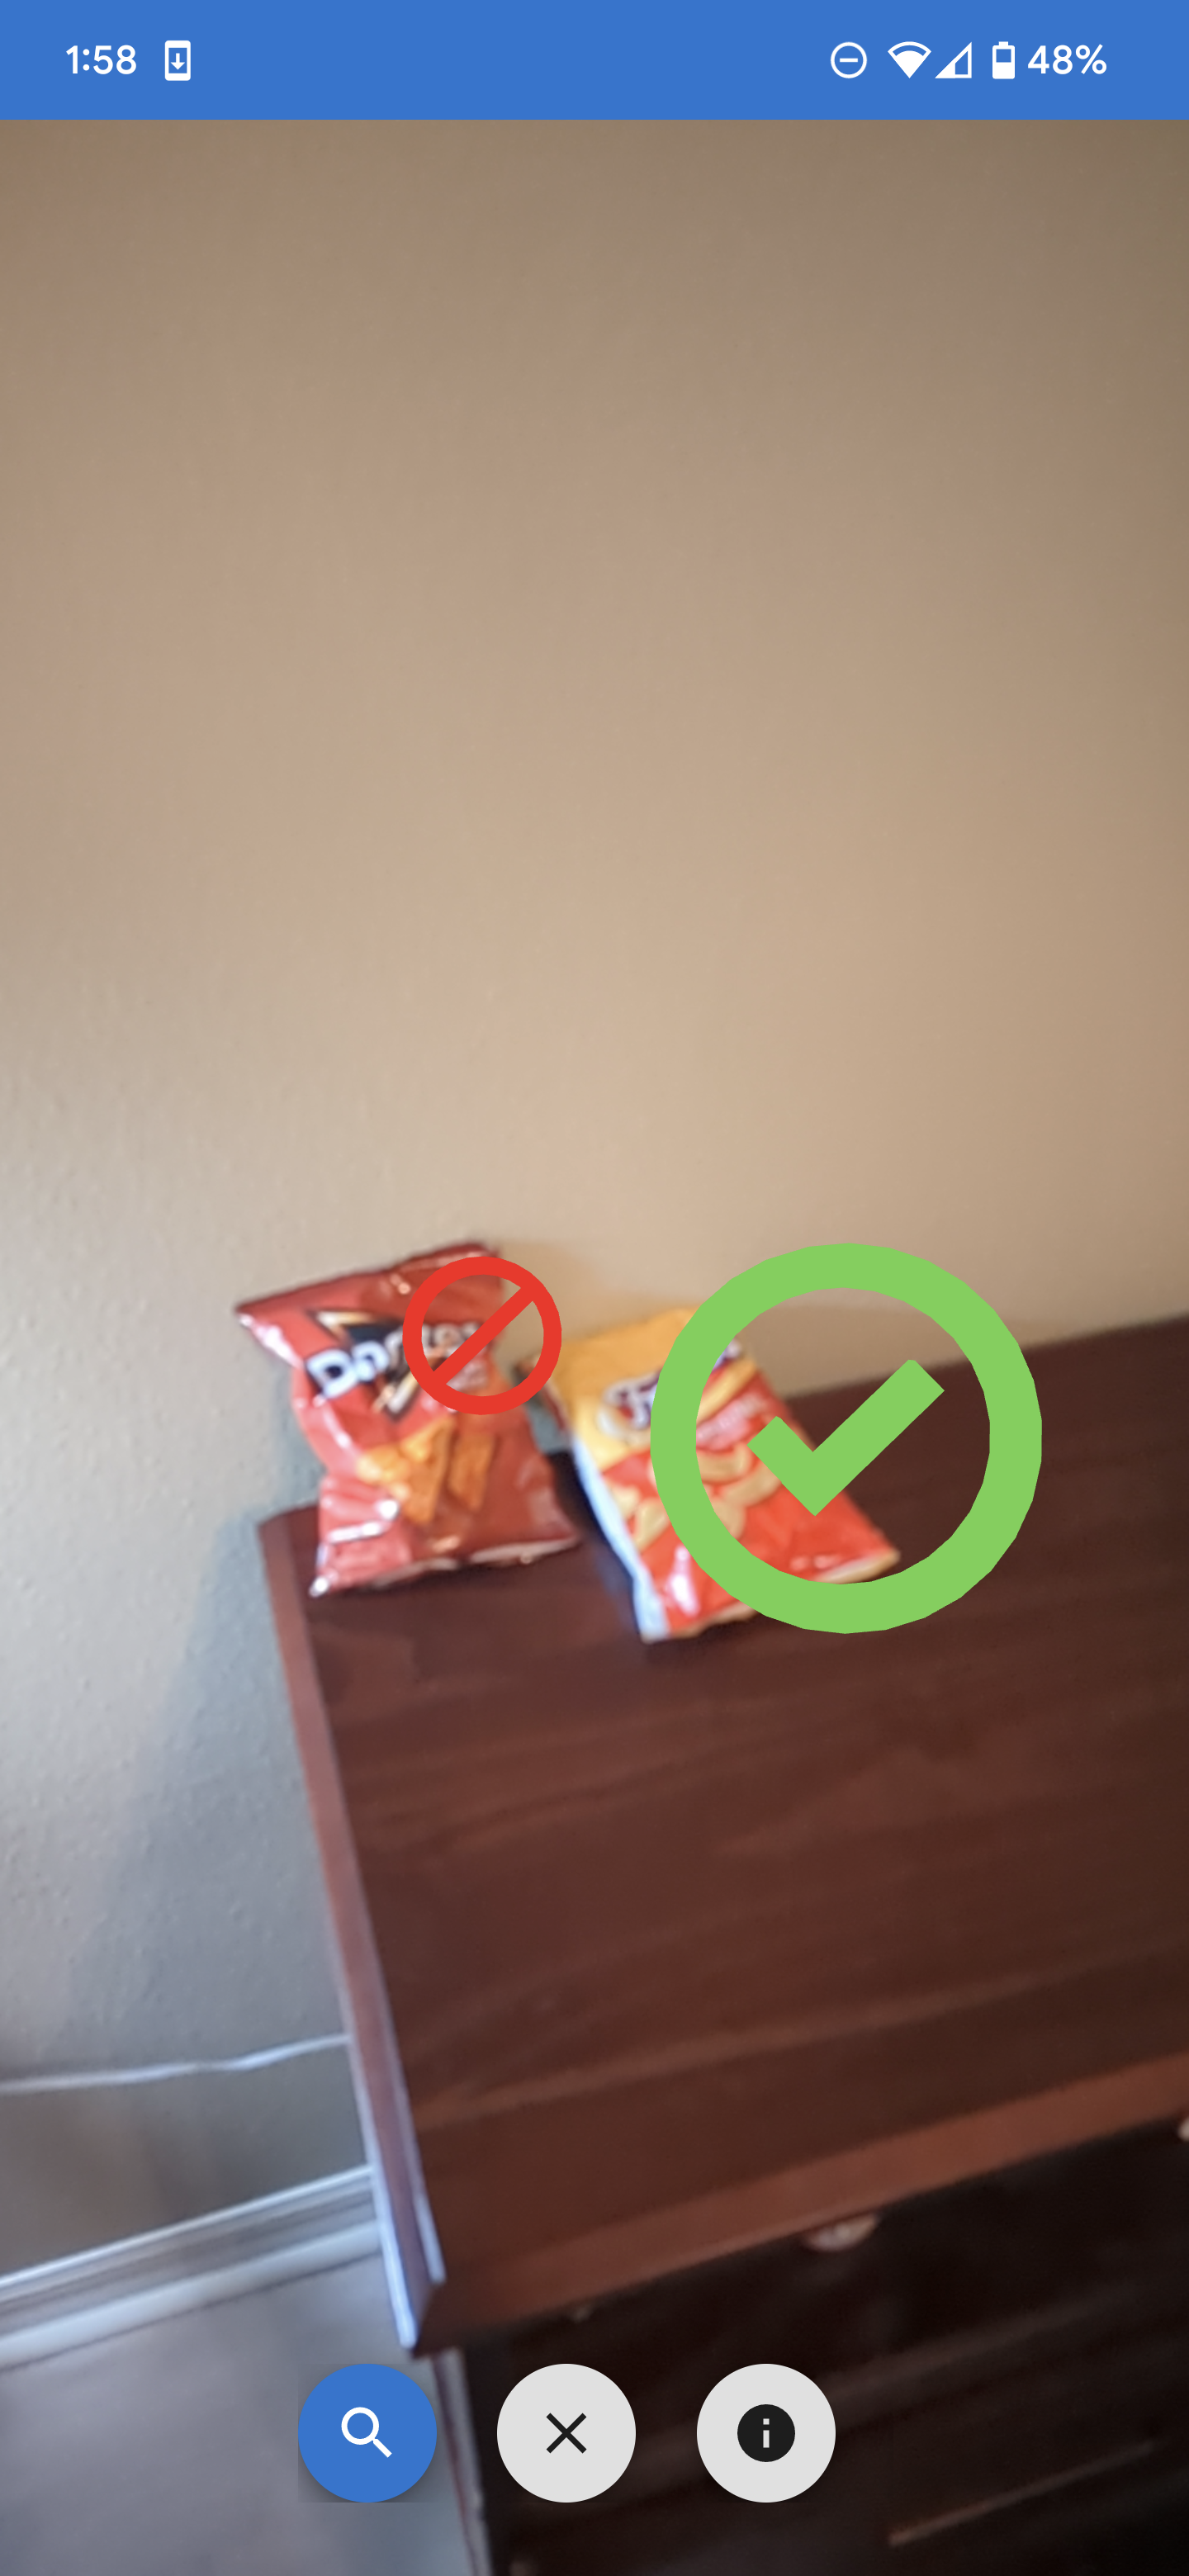
\includegraphics[width=\textwidth]{Images/red-and-green.png}
        \caption{Safe and Warning markers}
        \label{fig:safe-mark}
    \end{subfigure}
    \begin{subfigure}[]{0.3\textwidth}
        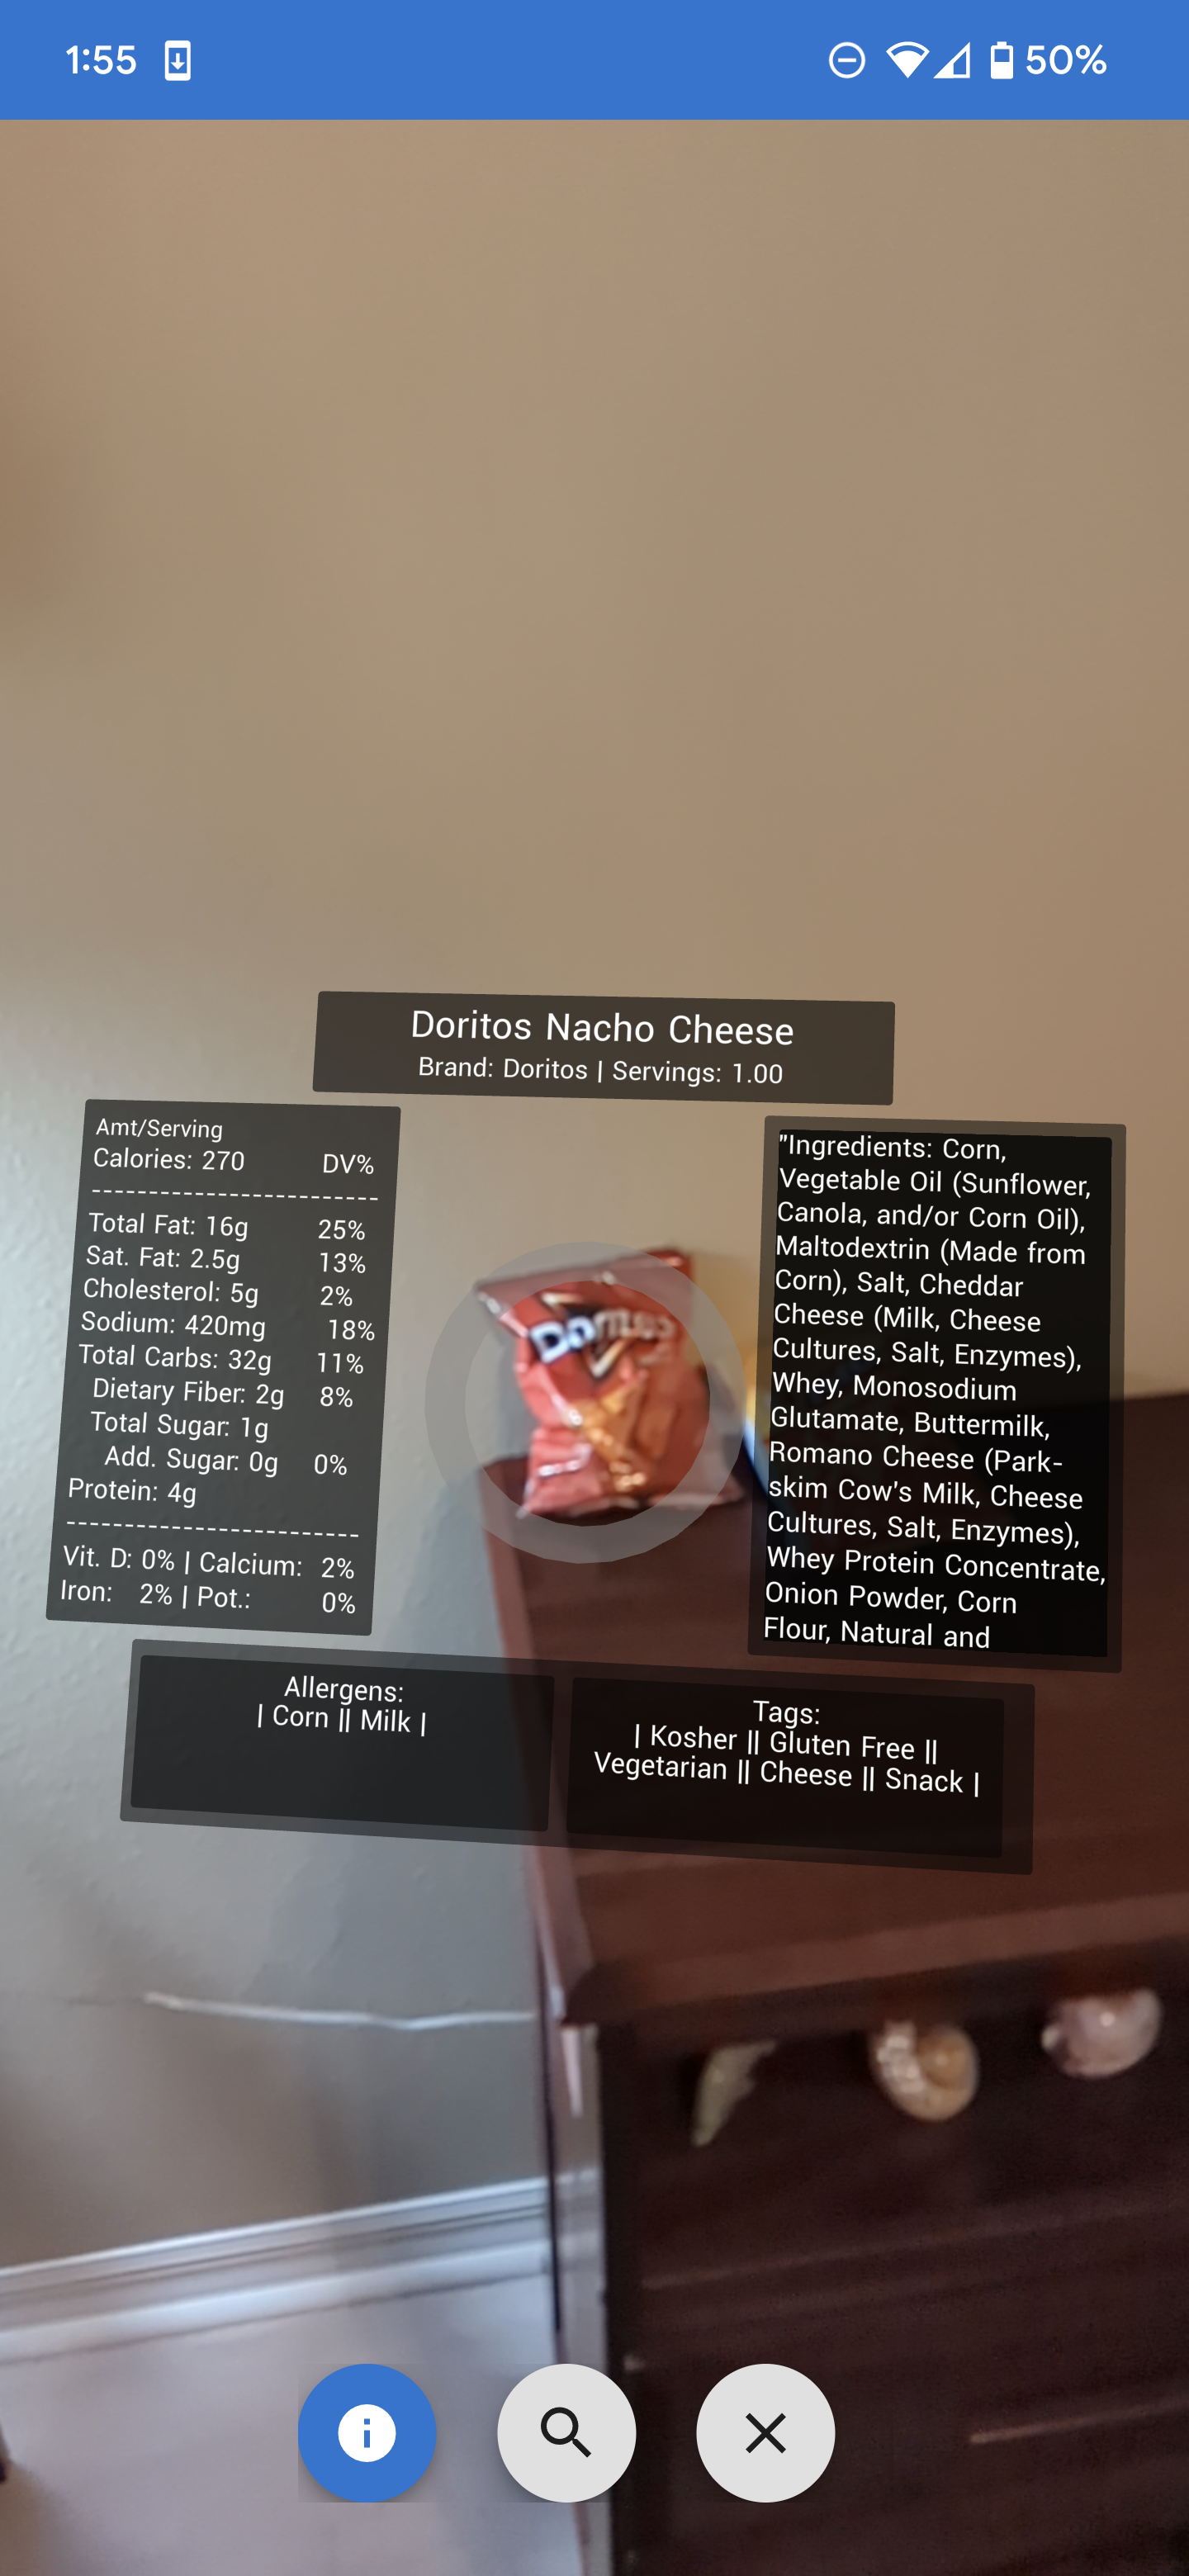
\includegraphics[width=\textwidth]{Images/menu-open.png}
        \caption{Nutrition menu}
        \label{fig:open-menu}
    \end{subfigure}
    \caption{Augmentation \acrshort{ui} examples}
    \label{fig:augment-ui}
\end{figure}

The nutrition menu system uses a library named "three-mesh-ui" to generate the virtual menus. The menus look good and are easy to read, but the library itself has some stability issues, and future work could be done to use Three's built in HTML rendering system instead of "three-mesh-ui." 
We designed the menu to display information in a format that was similar to a traditional nutrition label, and included all the serving size, allergen, and item tag information. We also left a large window in the center of the menu so users could see the item they were viewing directly, as shown in Figure \ref{fig:open-menu}. There were issues with the menu rotation during the first user study that were fixed by the second. We attempted but failed to implement scrolling for the ingredient menu, however, resulting in incomplete data visibility during both tests. %% ***ahamam*** add screenshots 
\paragraph{Menu Overlay}
WebXR has a feature named "DOM-overlay," allowing for the display of HTML elements over the XR canvas. We utilized this feature to build the user interface that controlled the search queries to the database, and to set user preferences for diet and allergies. We took inspiration from the carousel UI elements in popular \acrshort{ar} and camera focused apps such as Snapchat and the Google camera app to create the main mode selection UI. 
\begin{figure}[h]
    \centering
    \begin{subfigure}[]{0.3\textwidth}
        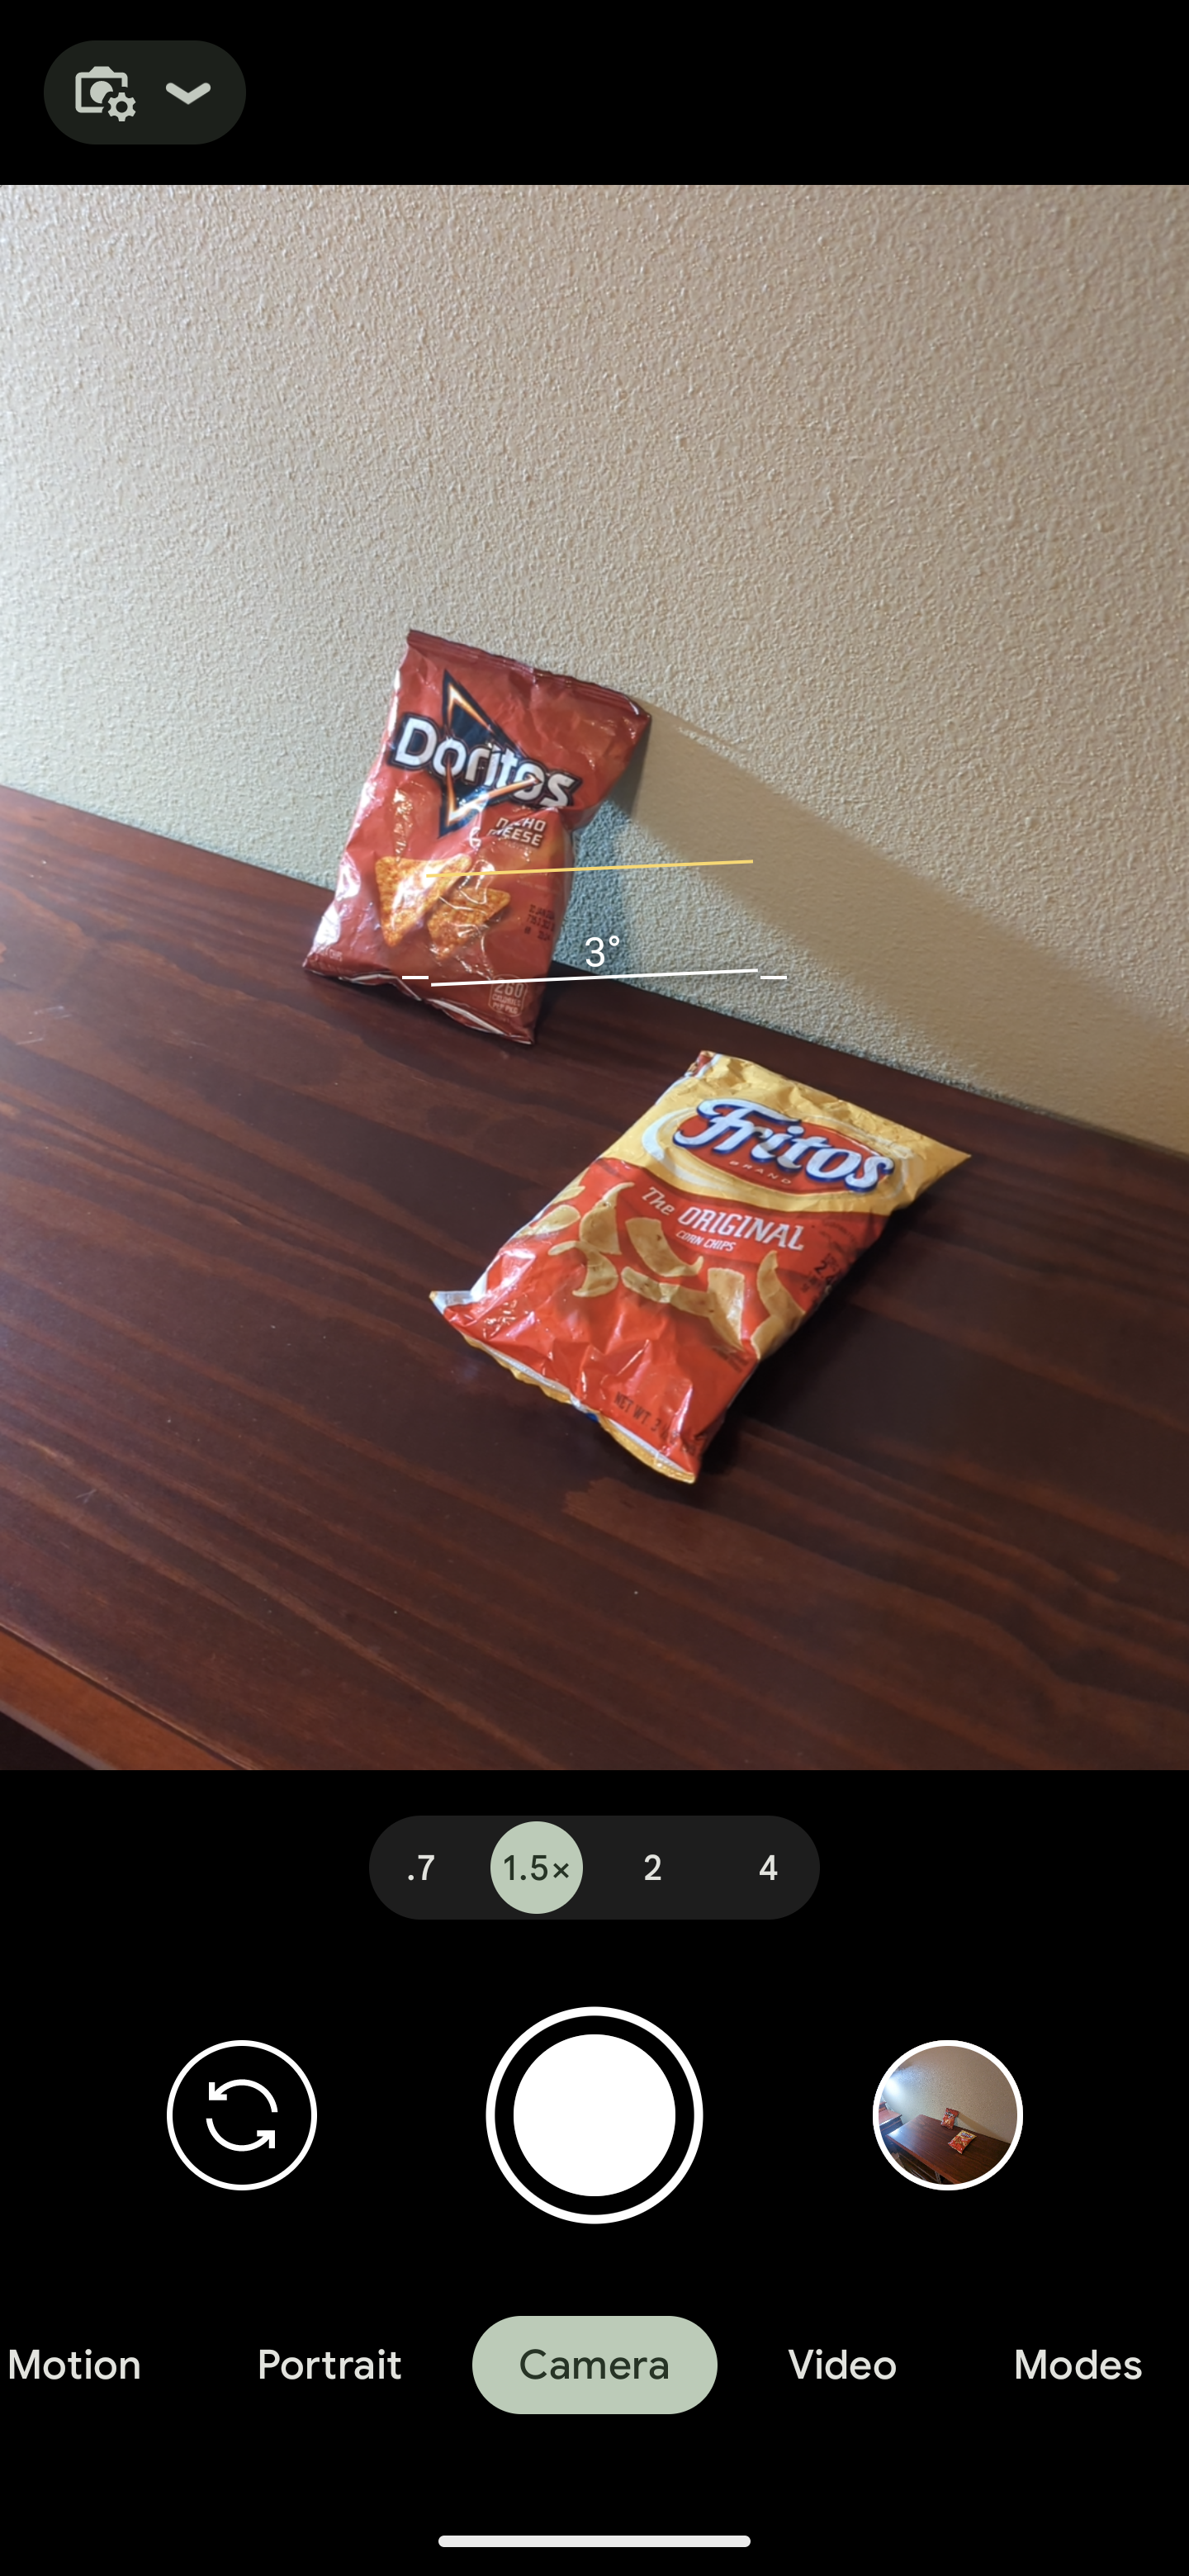
\includegraphics[width=\textwidth]{Images/google.png}
        \caption{Google Camera UI}
        \label{fig:google-ui}
    \end{subfigure}
    \begin{subfigure}[]{0.3\textwidth}
        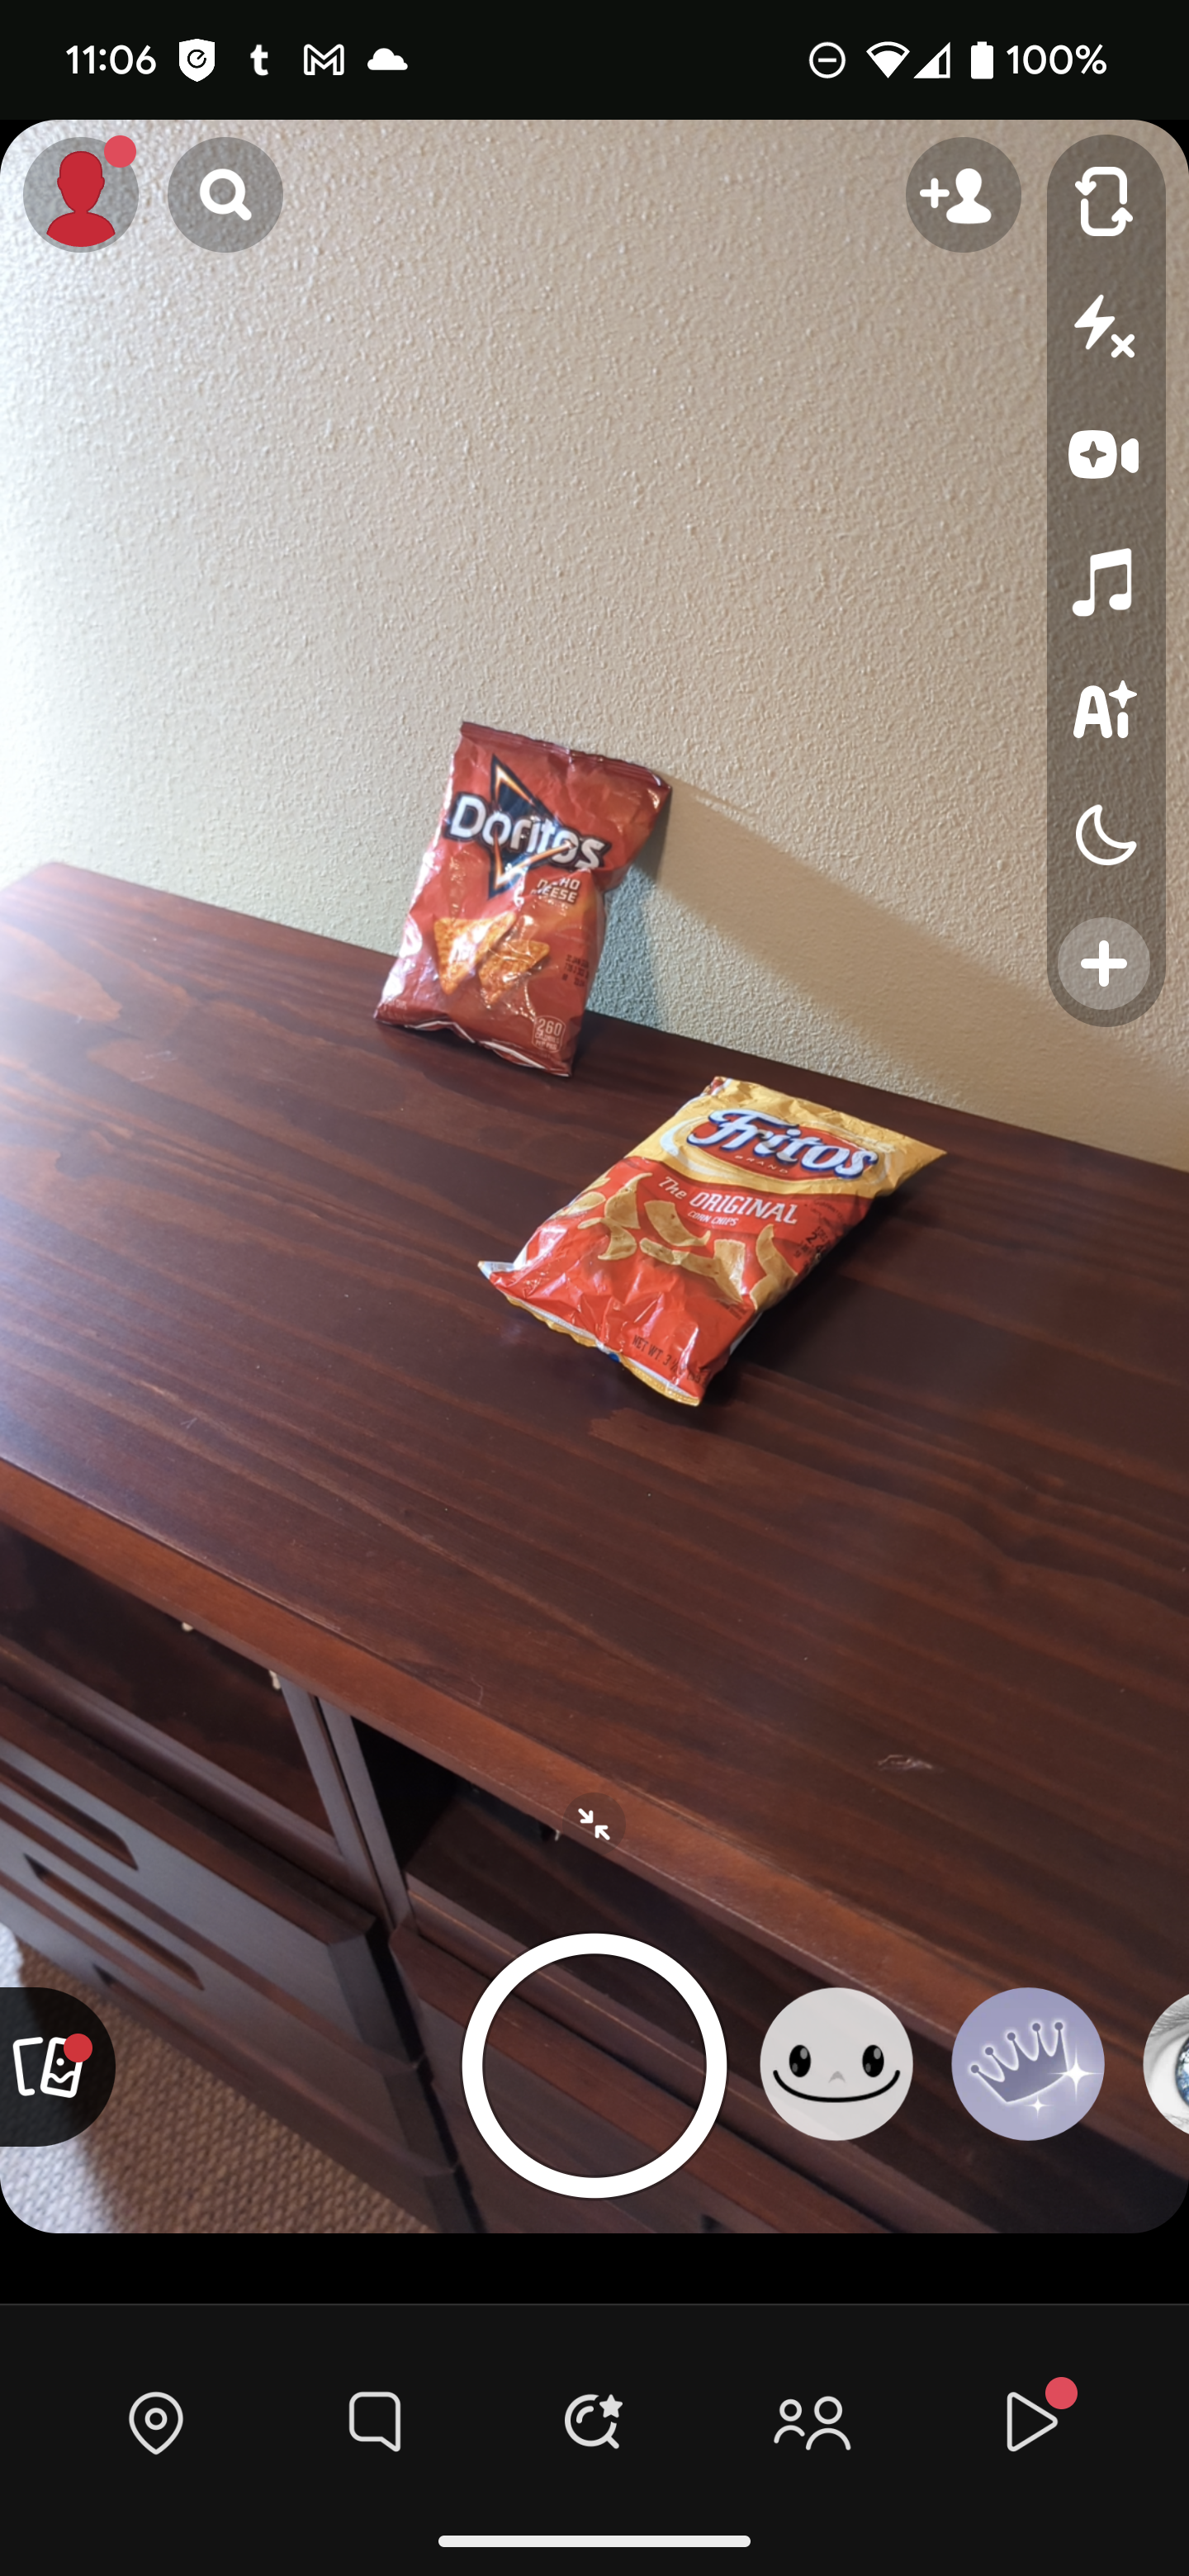
\includegraphics[width=\textwidth]{Images/snap.png}
        \caption{Snapchat (Snap) UI}
        \label{fig:snap-ui}
    \end{subfigure}
    \begin{subfigure}[]{0.3\textwidth}
        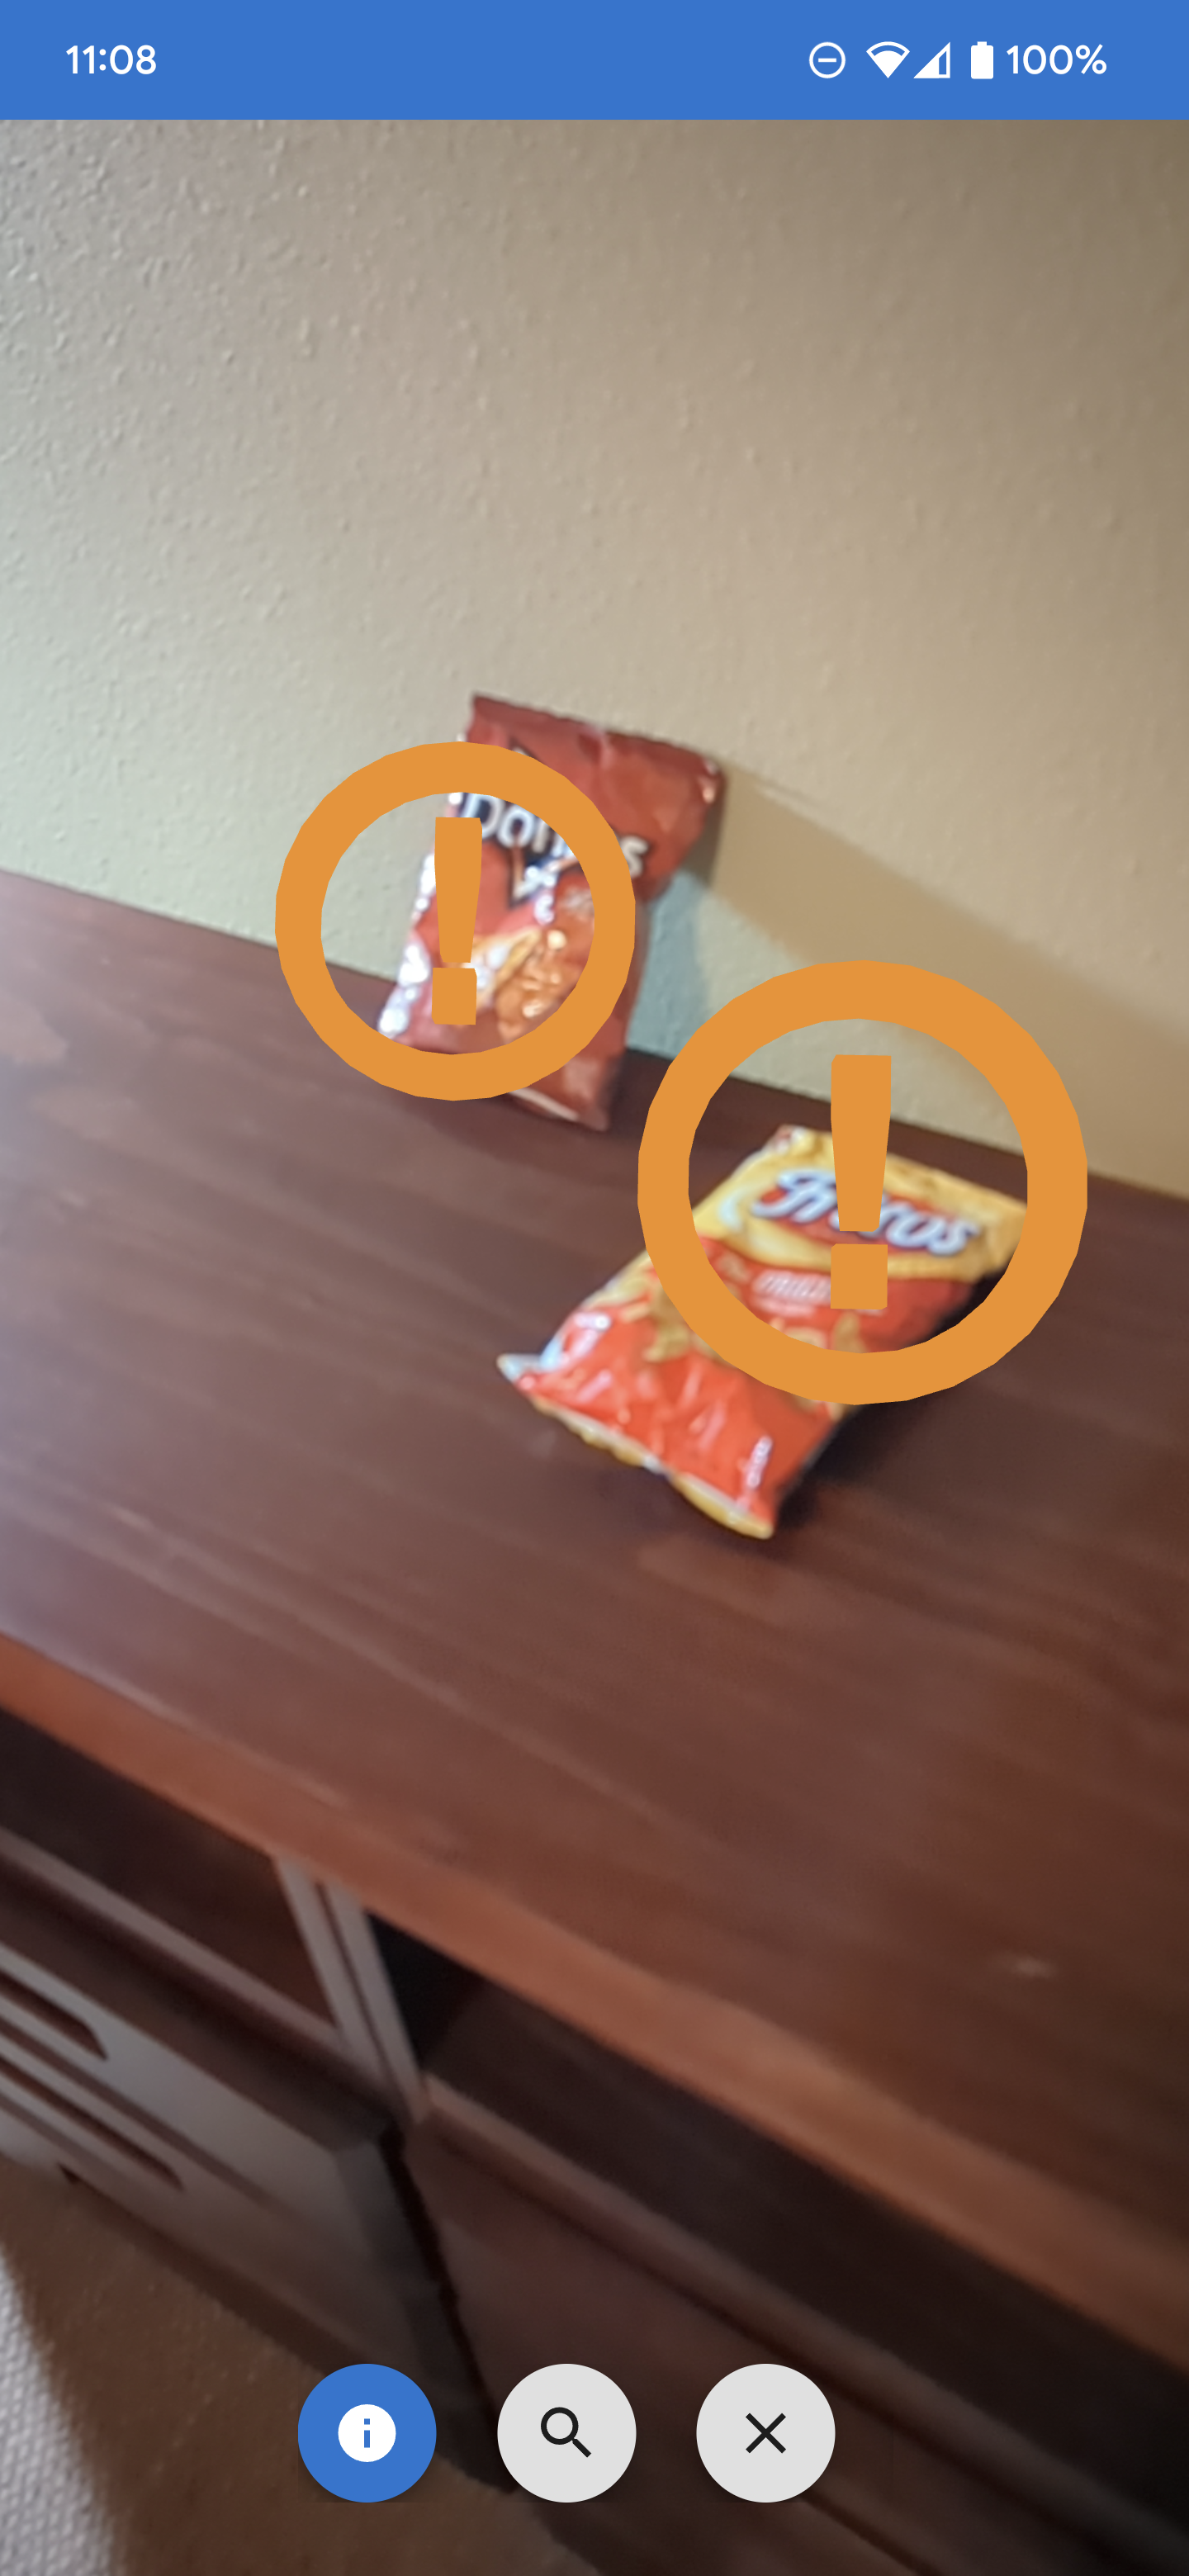
\includegraphics[width=\textwidth]{Images/item-findar.png}
        \caption{Item-FindAR (Ours)}
        \label{fig:itemfindar-ui}
    \end{subfigure}
    \caption{User Interface (UI) design inspiration}
    \label{fig:ui-comparison}
\end{figure}

Figure \ref{fig:ui-comparison} contains a side-by-side comparison of the three applications. We sought to minimize mental load by eliminating any unnecessary settings and features from the main view, maximizing the user's view of the space and leaving ample room for interaction with the virtual augmentations.

When users enter the \acrshort{ar} mode, a slider with three options (Info, Search, and Exit) appears at the bottom of the screen. Users can switch modes by sliding the carousel to one of the options or by tapping them directly. When a user taps on one of the icons, a popup menu appears with options to allow or deny various search attributes. %% ***ahamam*** elaborate more on how the inspiration from Goolgle and Snapchate is relevant. Place screebshots after the paragraph 
\filbreak
We used Material UI 5 for the interface, with Chip styled tags that users can toggle to include or exclude the different options. Users can directly search for items by name, or they can choose from a range of other options including tags, ingredients, allergens, and dietary restrictions. 
\begin{figure}[h!]
    \centering
    \begin{subfigure}[]{0.45\textwidth}
        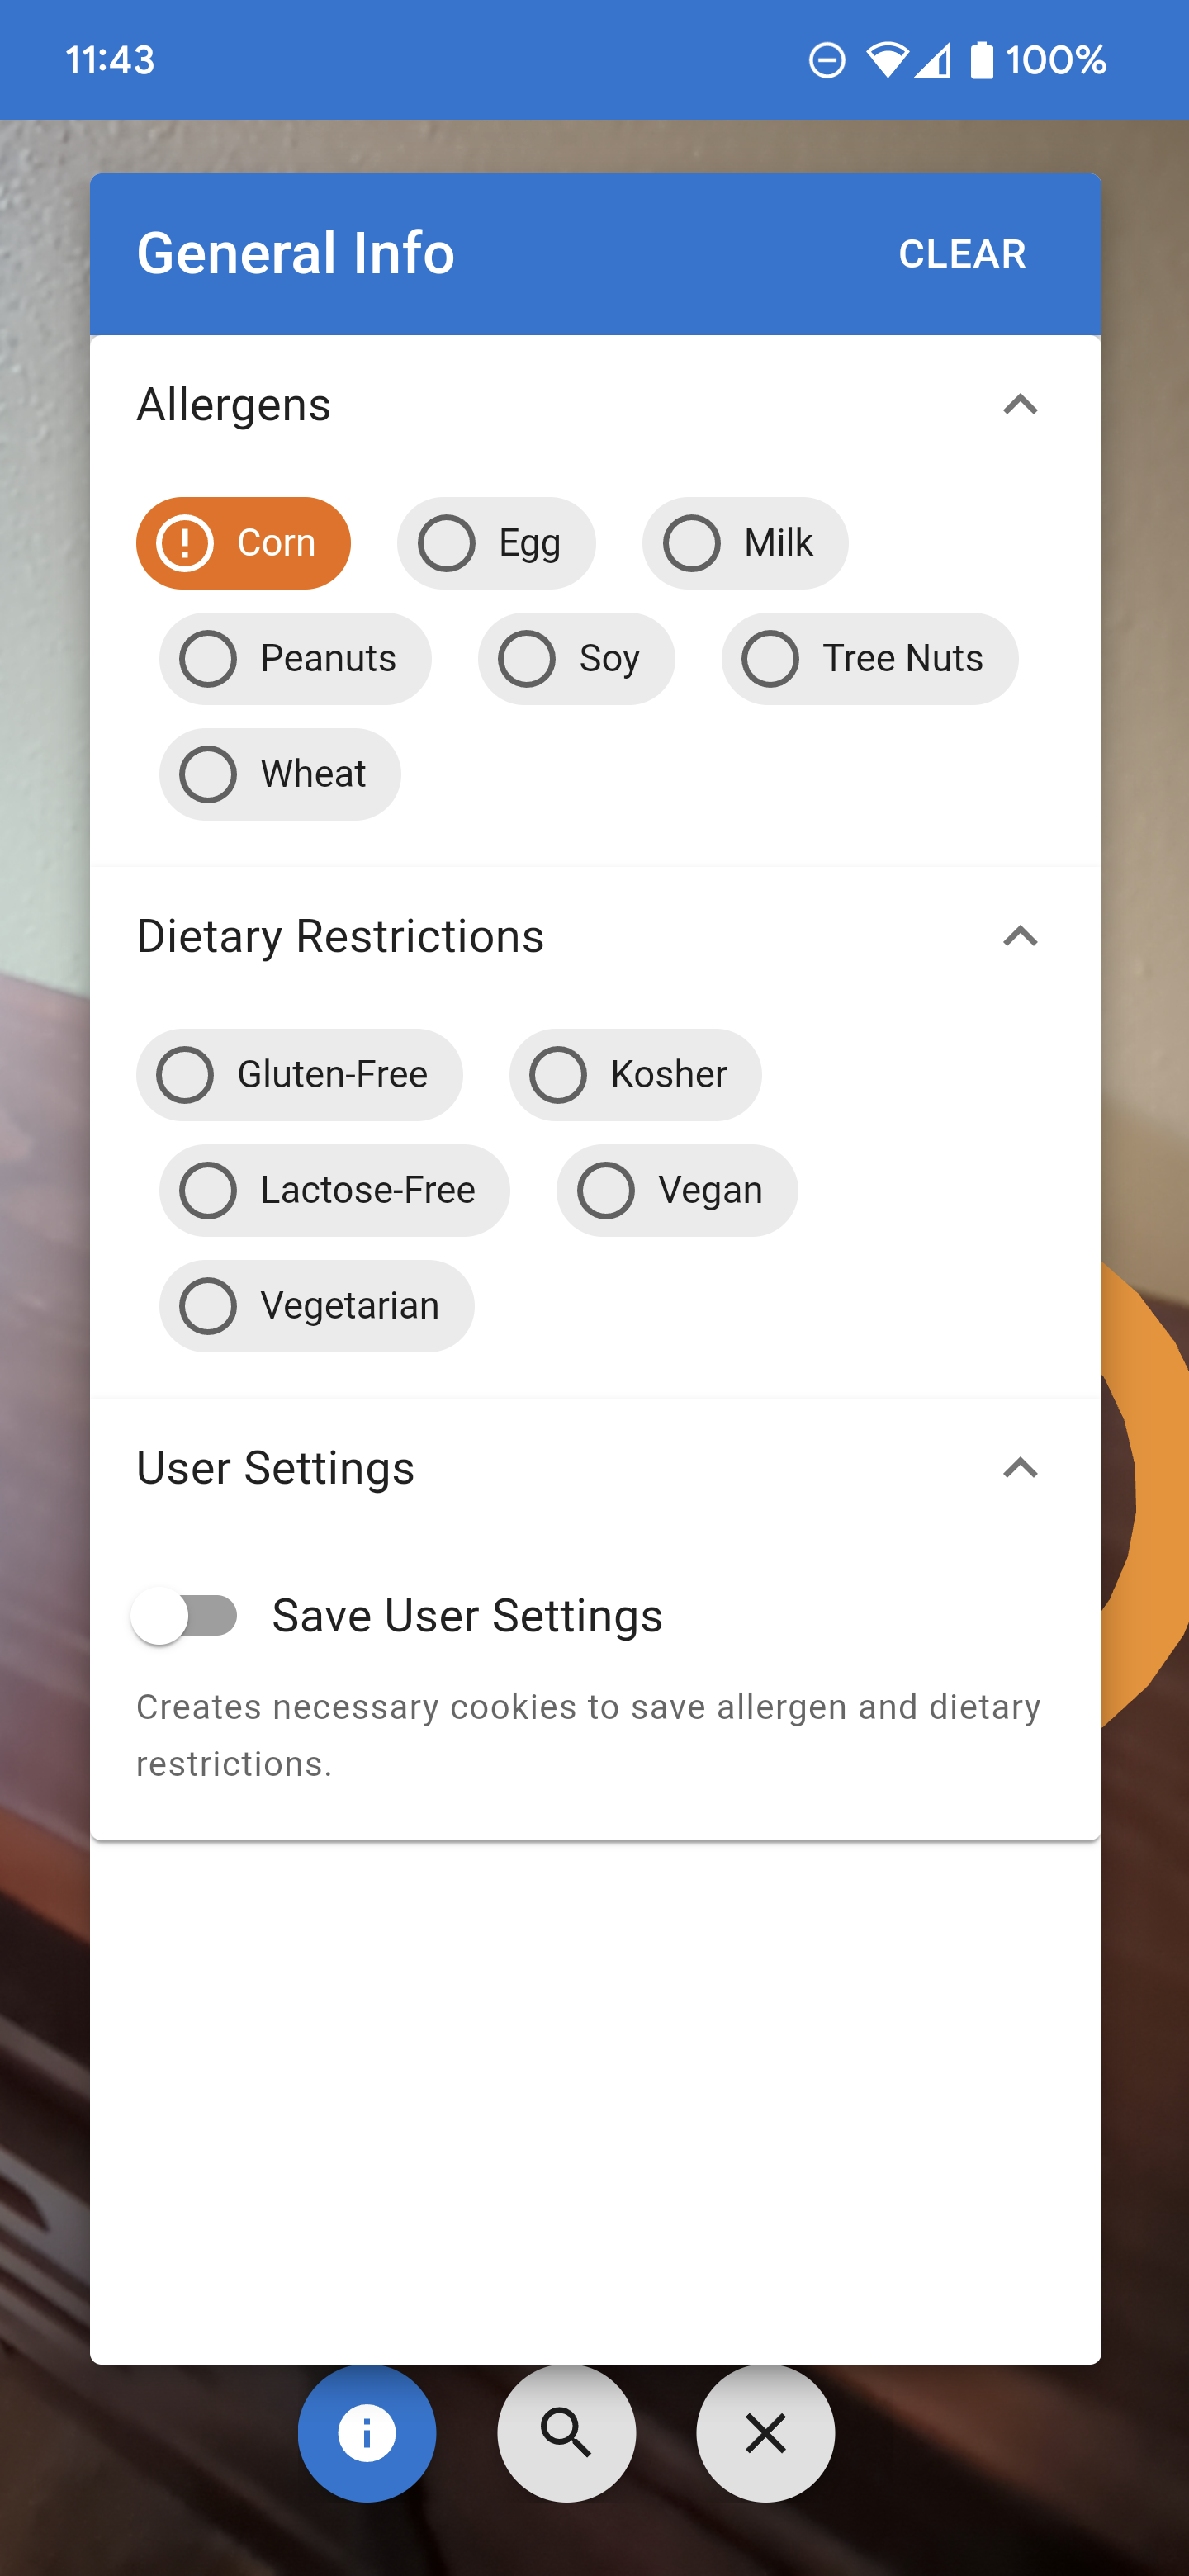
\includegraphics[width=\textwidth]{Images/info-ui.png}
        \caption{Info UI menu with "Corn" set to "Mild"}
        \label{fig:info-ui}
    \end{subfigure}
    \begin{subfigure}[]{0.45\textwidth}
        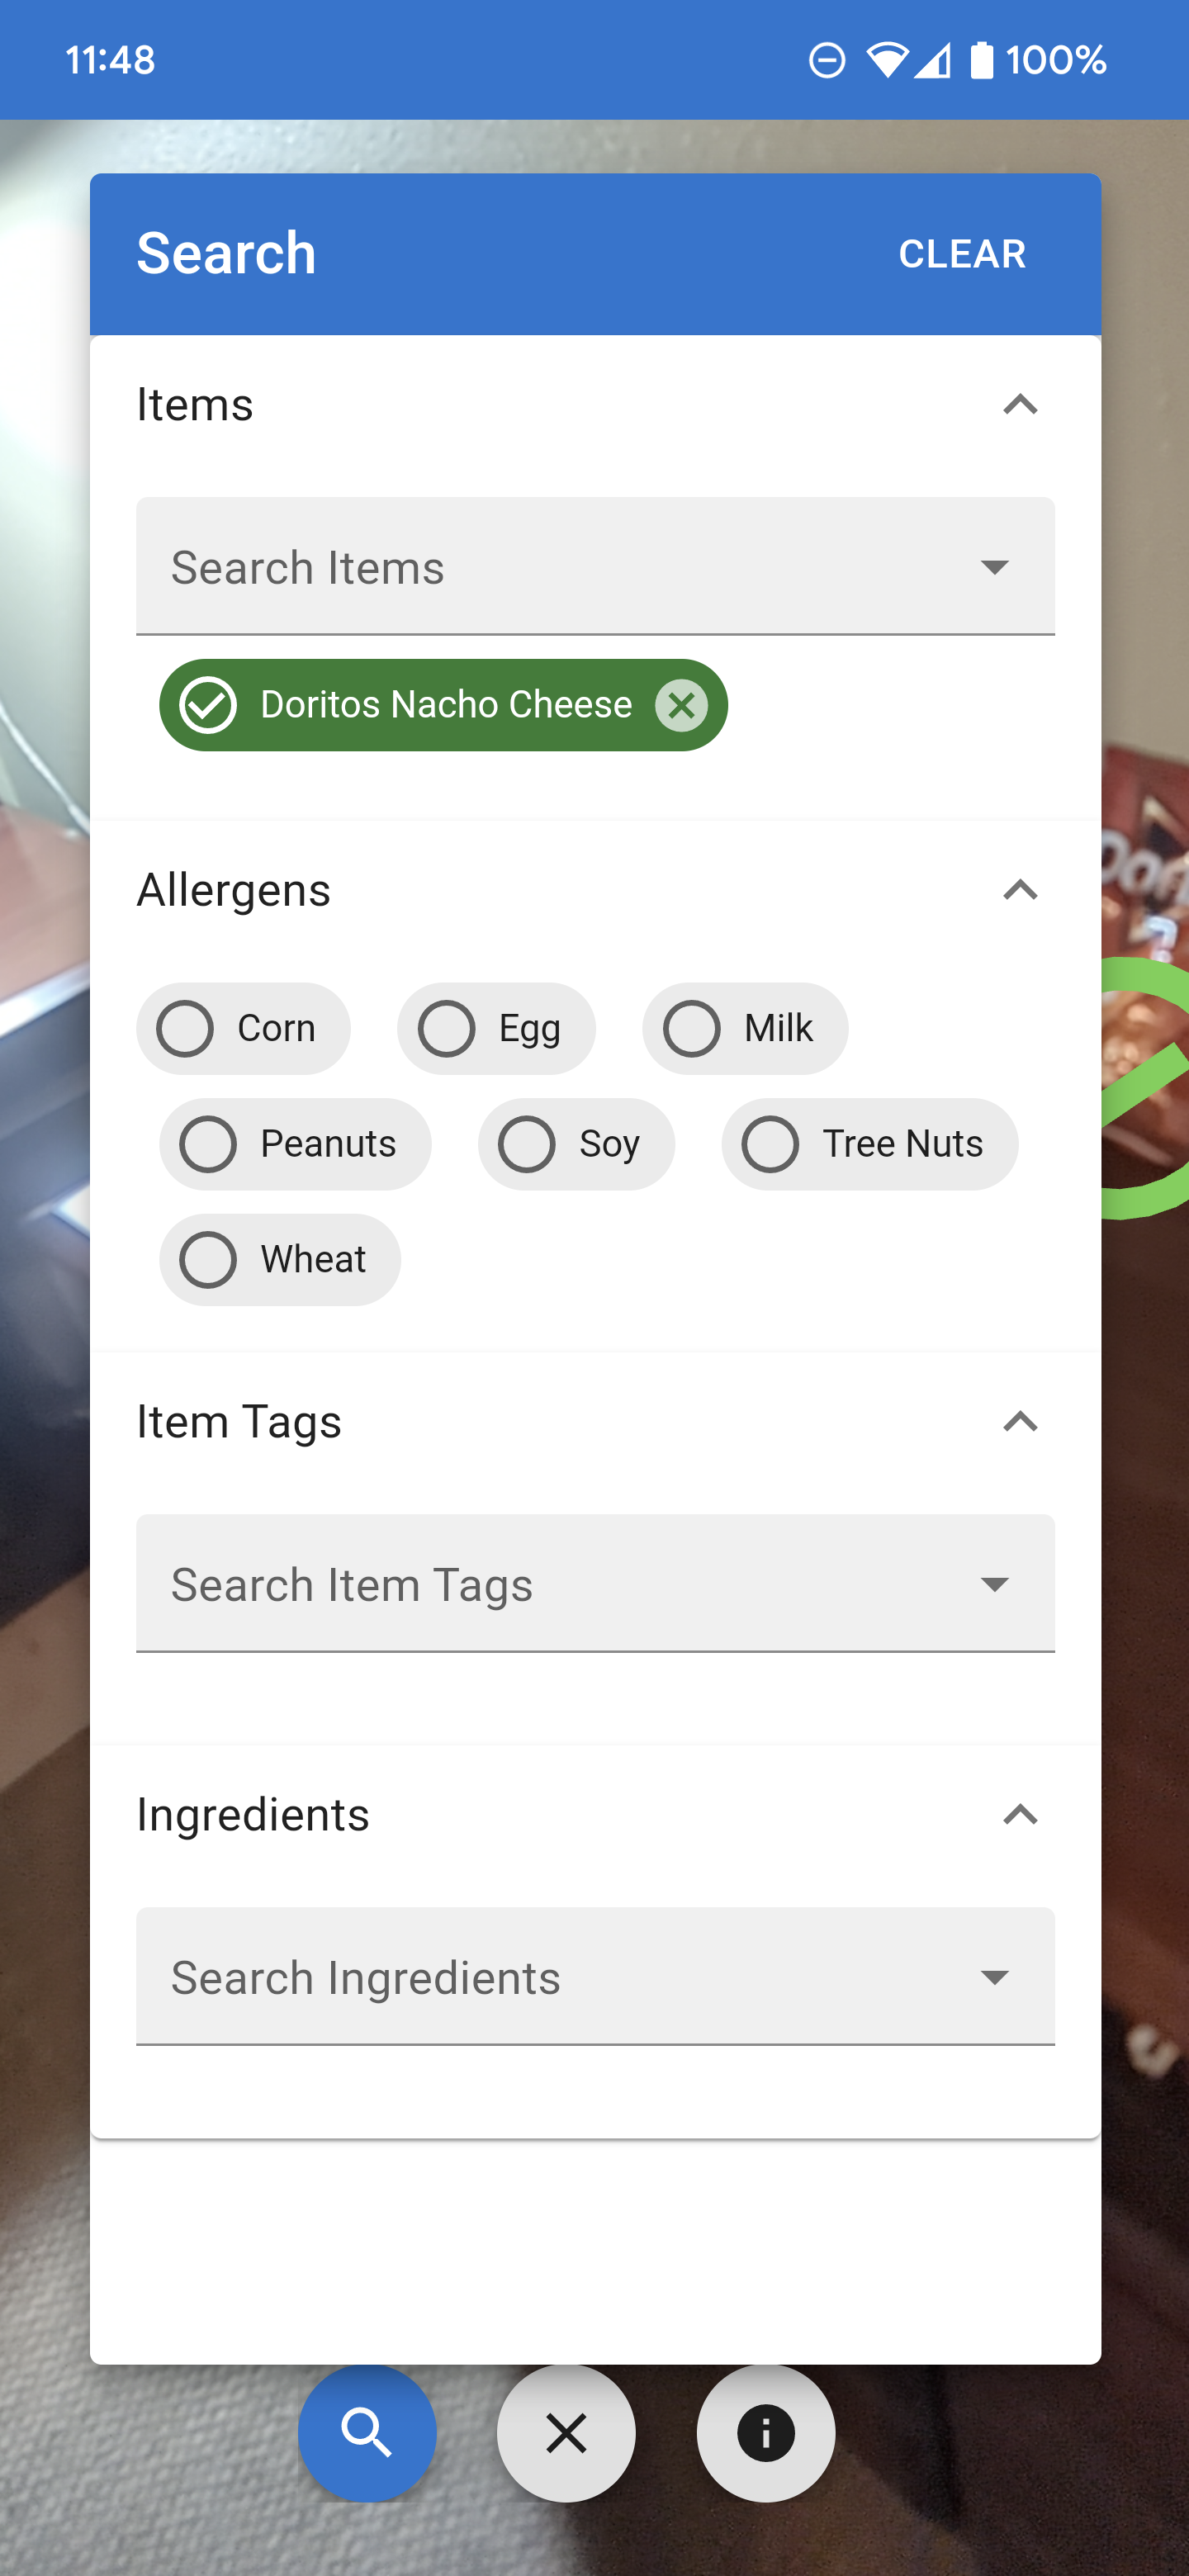
\includegraphics[width=\textwidth]{Images/search-ui.png}
        \caption{Search UI menu}
        \label{fig:search-ui}
    \end{subfigure}
    \caption{UI overlay menu comparison}
    \label{fig:mode-comparison}
\end{figure}

Users also have the option to enable a cookie to save their preferences, and the option can easily be toggled off, deleting the cached information. 
In "Info" mode, any items detected are displayed to the user, with varying markers depending on the user's set allergen and dietary information. In "Search" mode, allergen and dietary user settings are still considered, but only items matching the search options are displayed. 
Users can type the options they're looking for in the Search menu, but there are instability issues with the resizing of the canvas that occurs when the keyboard opens. A better option would be overlaying the keyboard, but we ruled this as out of scope for the current project.
\filbreak
\begin{samepage}
\section{Data Analysis Methods}
We collected three types of data from participants: 
\begin{itemize}
    \item NASA's \acrfull{tlx} 
    \item the \acrfull{sus}
    \item a combination of open ended and multiple-choice survey questions to identify user opinions of the two versions
Some of the questions were poorly written or required additional explanation to participants for clarity. We have adjusted some of the results to reflect the intention of the question despite the limited ability to answer or unclear instructions. The methods for analyzing the data are described below.
\end{itemize}

\end{samepage}
\subsection{Qualitative Data Analysis}
We administered four different surveys during the user testing, two for each study. Questions included yes/no, multiple choice, rankings/ratings, and open-ended questions. We used textual and thematic analysis to develop a set of relevant code words and themes that represent aspects of our research questions. We then assigned relevant codes to each participant's responses and looked for patterns to assess what the greatest concerns were, what improvements were needed for future iterations, and whether the system provided meaningful value to the people testing it. Results are compared as bar charts sorted by the most common theme for each study. We converted the data to percentages of the sample sizes to better compare the results. 

\subsection{Quantitative Data Analysis}
Participants completed the TLX and the SUS after each test. Five participants from the first study participated in the second study, providing opinions on how the system improved between the first and second studies. 
\subsubsection{NASA TLX}
The NASA Task Load Index measures workload, the cost to the person using the system, across six measurements: Effort (E), Frustration Level (FL), Mental Demand (MD), Performance (P), Physical Demand (PD), and Temporal Demand (TD). The survey consists of three steps: 
\begin{enumerate}
    \item Participants rank from low to high how well each measurement represents their experience
    \item Participants rank which measurements had a greater impact
    \item Participant scores are weighted based on their measurement rankings
\end{enumerate}
\filbreak
This generates two types of scores: 
\begin{itemize}
    \item Individual weighted scores for each measure
    \item Weighted Work Load (WWL) score
First, we averaged all the participant scores for each measure to identify which ranked the highest. The highest scoring factor is the main source of workload for surveyed participants. Multicollinearity is the state when multiple independent variables are correlated, positively or negatively, reducing the model's reliability. We performed the Pearson Correlation to identify any possible one-to-one relationships and the Coefficients of Regression Significance Test to assess whether any of the measures were significant enough for use predicting the major source of load.
\end{itemize}

The WWL average score is subjective and lacks the context required to accurately predict or judge the actual workload in a consistent way across different use cases and studies, leading to a lack of standardized ratings. The score can range from 0 to 100, and lower is better. The score is useful as a metric for how the user experience changes between versions.
\subsubsection{SUS}
The System Usability Survey is a ten question survey that accurately assesses the usability of nearly any system, ranging from hardware to software. Results correlate highly to letter or adjective scales, and a standardized set of interpretation guidelines was compiled by \cite{brooke_sus_1996} and are listed in Figure \ref{fig:sus-table}. Generally, the individual user scores should not be considered for assessment, only the average for the group. We plot the scores for both studies in Figure \ref{fig:sus-plot} to show the change in scores between the two versions.

\begin{figure}[h]
    \centering
    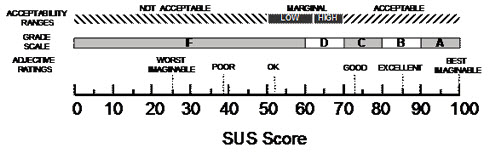
\includegraphics[width=0.8\textwidth]{Images/sus-table.jpg}
    \caption{Alignment of SUS scores and adjective/letter grade scales.}
    \label{fig:sus-table}
\end{figure}

\chapter{User Studies}
We conducted two user studies for this thesis. The first used the minimal working concept we had finished at the time, and the second used the final version a year later. The testing procedure and questionnaire styles were the same for both studies.
\section{User Study 1: Early Version Testing}
For the first study, we had implemented the object recognition and the item marker/menu systems, but lacked the search and navigation UI. There were several major issues and missing features, including temporary marker models and textures, alignment offset issues, and incorrect menu rotation, as shown in Figure \ref{fig:ui-issues-v1}.

Tests were conducted in the assigned lab space, using the labset model. All systems (the client, DB, and CV server) were run from the same laptop, and participants were given a Google Pixel 6XL smartphone to perform the tests with. We connected to the web app directly by IP over the local WiFi network.
\subsection{Participants}
The first study had twelve participants, ten males and two females. Ages ranged from 18 to 76. Participants were mainly recruited from around campus via word of mouth and postings in student run message servers. Participants were offered an optional snack or beverage as an incentive. The elderly parents of one of the researchers also participated, providing the perspectives of possible users for a more generalized version of our application.
\begin{figure}[h]
    \centering
    \begin{subfigure}[]{0.3\textwidth}
        \centering
        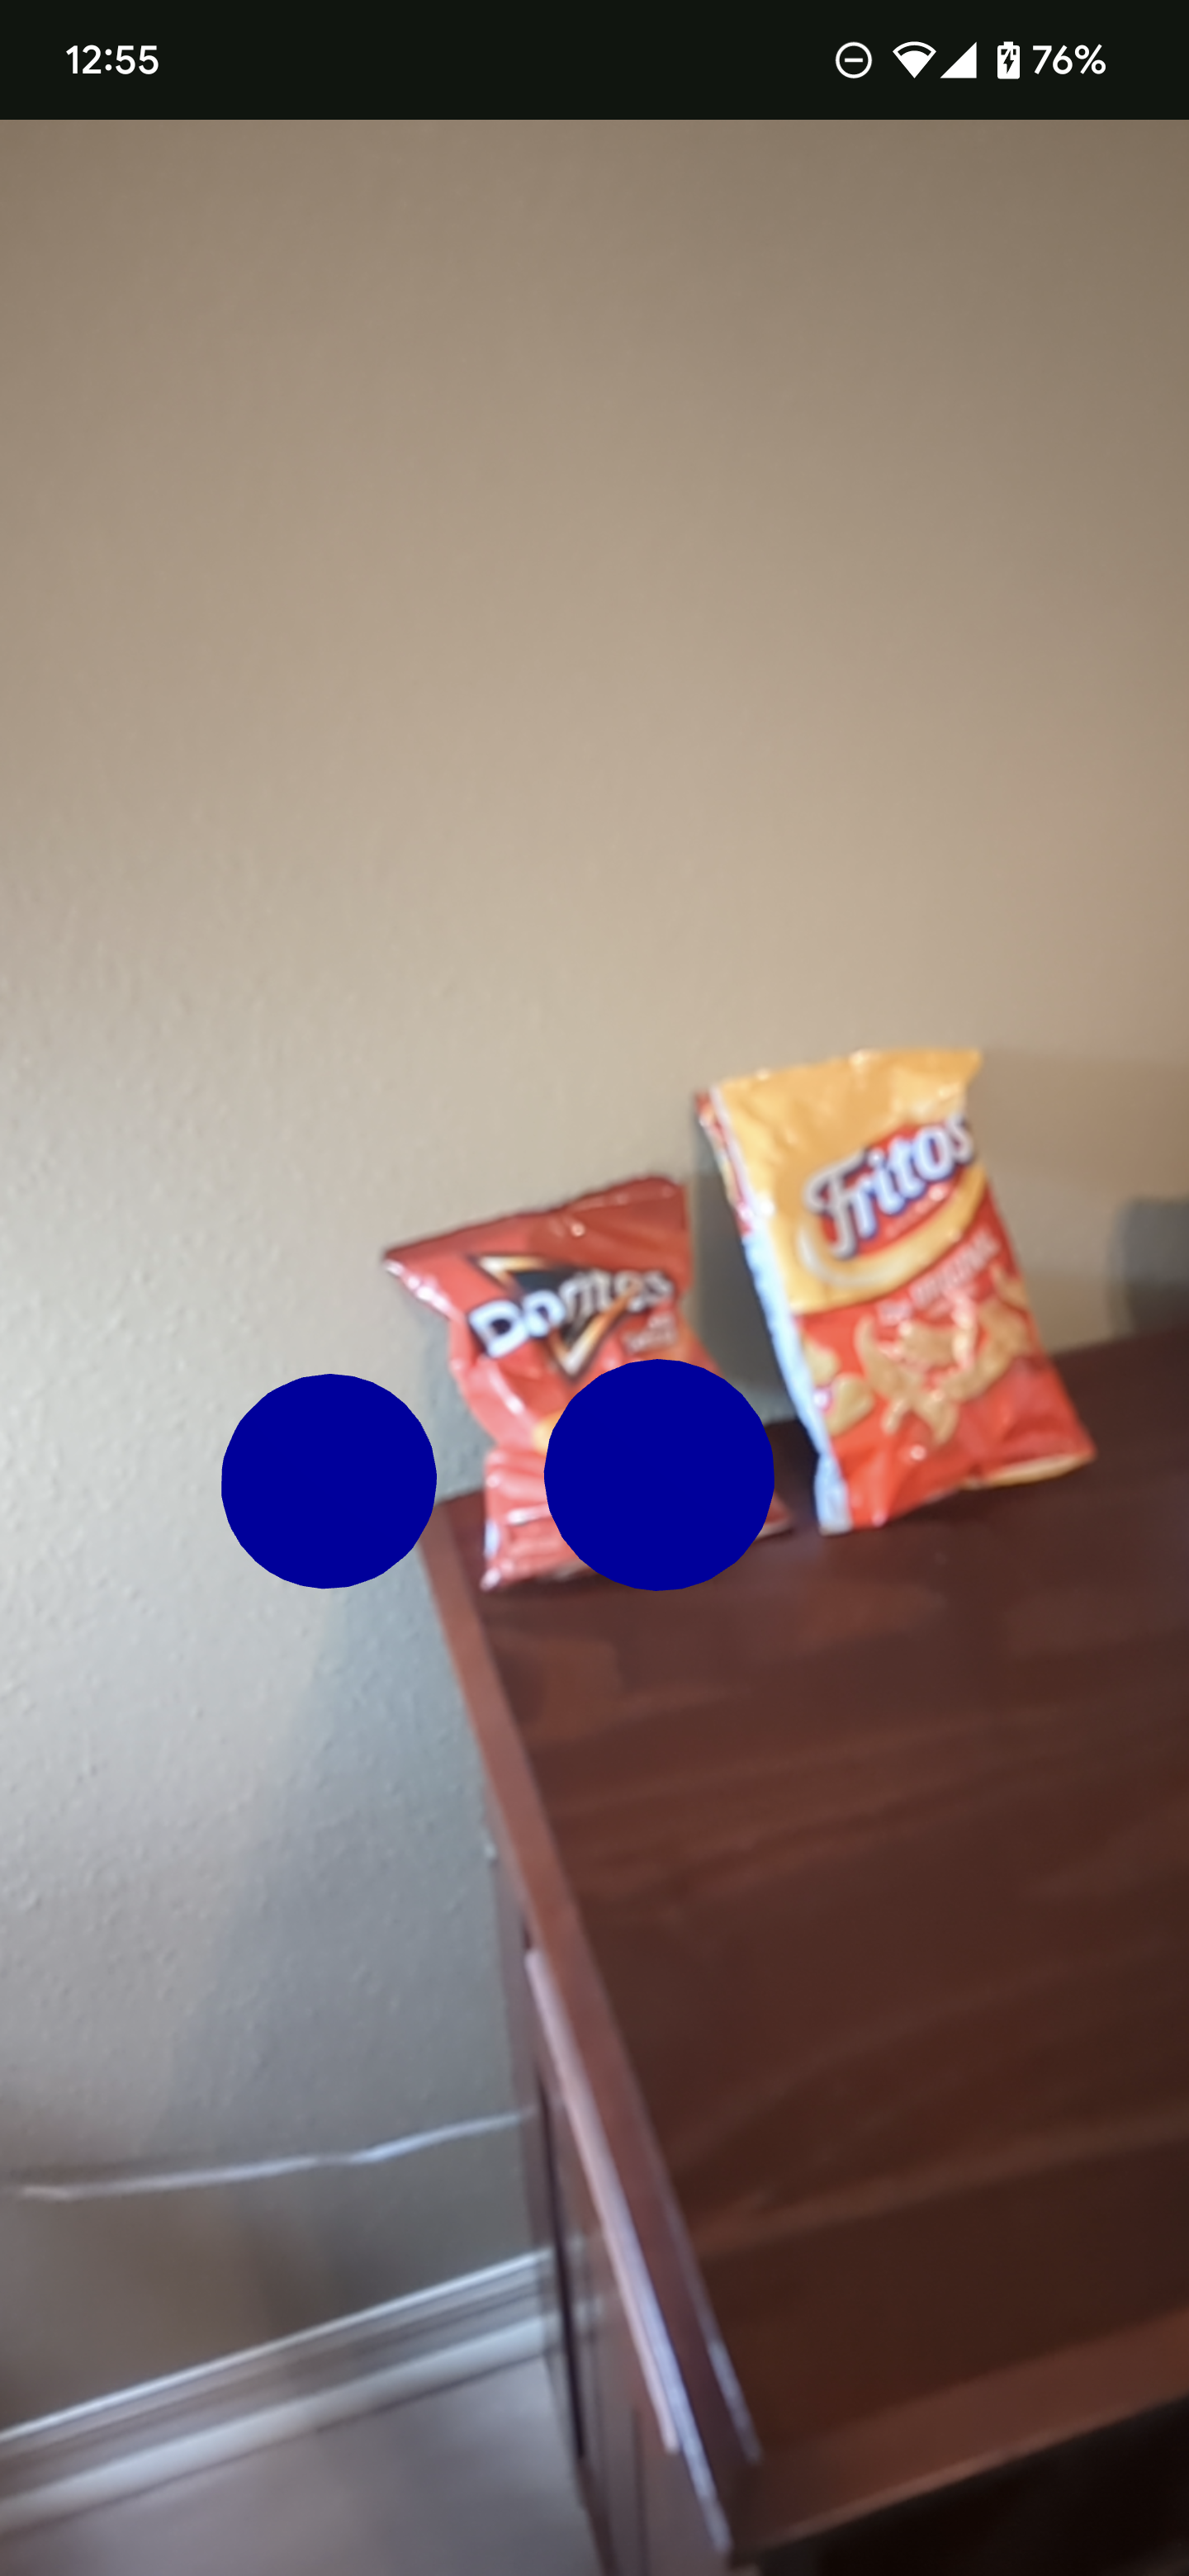
\includegraphics[width=\linewidth]{Images/markeralignment.png}
        \caption{Temporary markers with alignment issues}
        \label{fig:marker-alignment}
    \end{subfigure}
    \begin{subfigure}[]{0.3\textwidth}
        \centering
        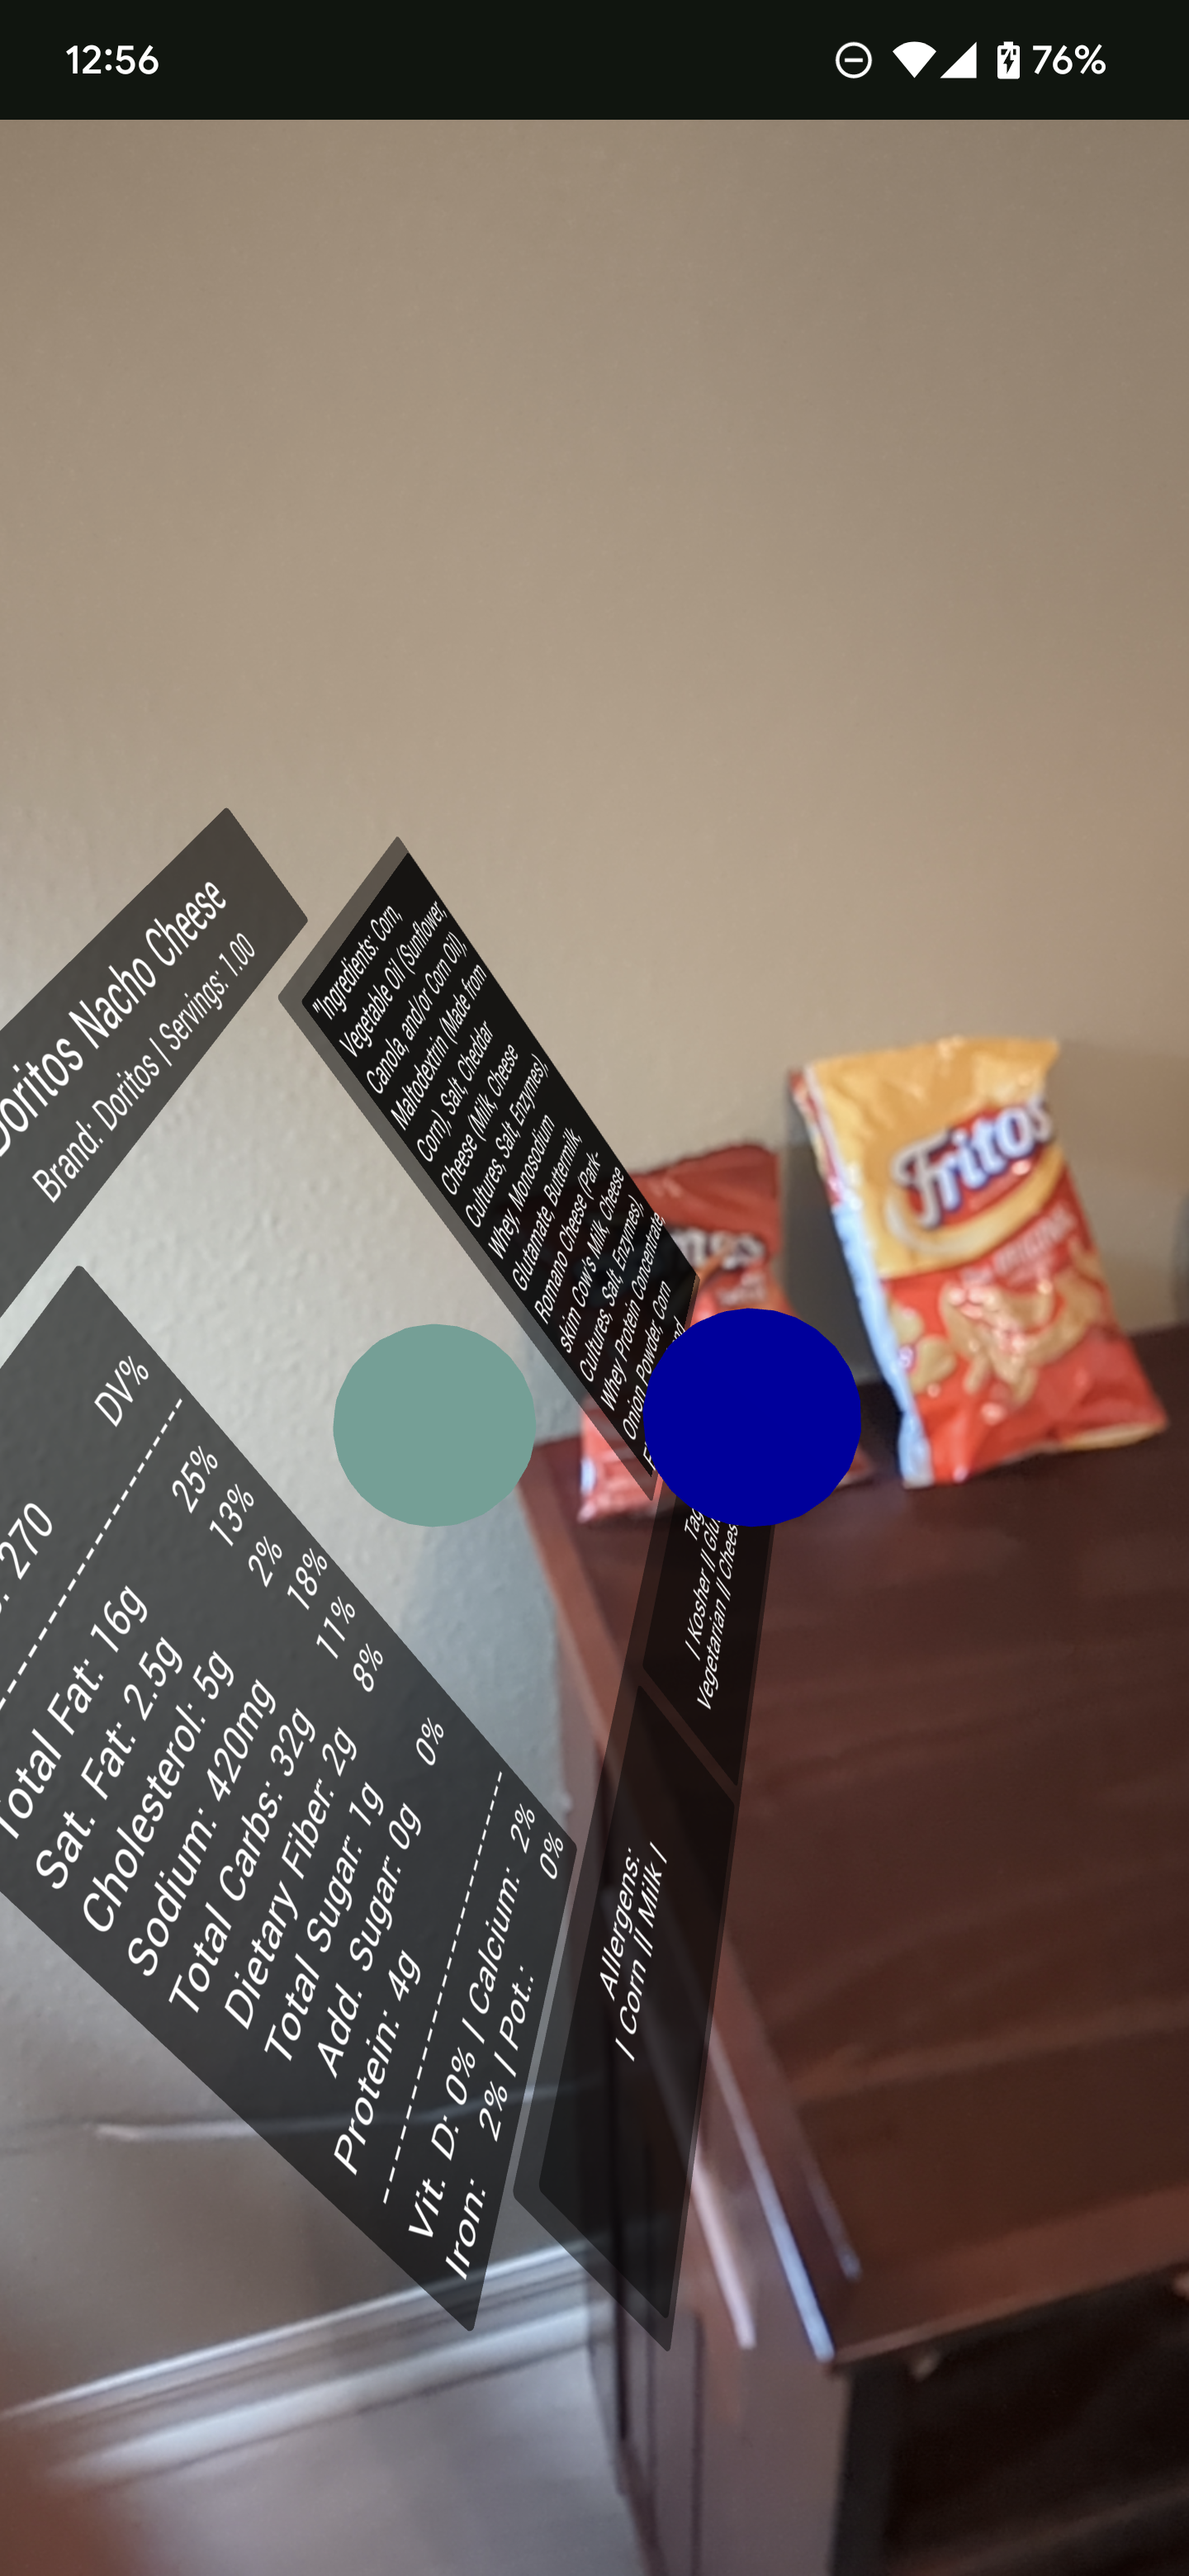
\includegraphics[width=\linewidth]{Images/menurotation.png}
        \caption{Incorrect menu rotation and marker occlusion}
        \label{fig:menu-rotation}
    \end{subfigure}
    \caption{Technical issues in Study 1}
    \label{fig:ui-issues-v1}
\end{figure}
\subsection{Procedure}
Prospective participants were first given an overview of the testing process and a brief explanation of the use cases. They were alerted to the unstable nature of the application and asked to focus on the overall concept rather than the implementation problems. They were presented with the first survey, and informed that they were giving consent to have their answers recorded and used, and that they could withdraw consent at any time. When finished with the first survey, participants were instructed to spend 5-10 minutes using the web app on the provided device. Users were presented with a list of different features to try and were allowed to freely use the app. Multiple issues including flashing of the screen occurred, causing many participants to quit before the time limit. Once the test had concluded, participants completed the final surveys and received their chosen snack item.
\subsection{Data Collection Methods}
Participant responses were collected from one survey before and two after the demonstration and testing period. User feedback during testing was not recorded; brief notes were made instead. Performance metrics for the \acrshort{yolo} model were recorded during training. 
\subsubsection{Usability Testing}
Participants completed two different usability surveys: the \acrfull{tlx}, and the \acrfull{sus}. Users first completed the \acrshort{tlx}, followed by the post-testing feedback survey and the \acrshort{sus}. 
\subsubsection{Surveys}
Questions for the pre-survey included general statistics, prior experience with similar apps, dietary and allergy restrictions, hygiene concerns, and label comprehension difficulty. The post-survey covered how users felt about the experience, whether there was an improvement over normal shopping, and whether the lack of a required app installation or user account was an appreciated feature. Participants were also encouraged to provide additional thoughts and opinions on both the concept and the implementation.

The post-trial survey asked participants to reflect on how the \acrshort{ar} system changed their shopping experience, whether the features offered were useful, whether they would use the application again, and what improvements they would like to see. We also asked them how the web experience affected their feelings about the app and if they were more likely to use the system as a result. The second part of the post-trial survey was the \acrshort{sus}. All surveys can be found in Appendix B.

\section{User Study 2: Final Version Testing}
The final testing version addressed many of the issues raised by participants in the first study. For this round of testing nearly all features from the initial design documents were implemented and functional. Table \ref{tab:feature-comp} compares the feature differences between versions 1 and 2. 

The locations for testing the second version included the lab, the upstairs IST, and one of the IST classrooms. Participants were allowed to use their own Android devices, and the web app client and DB were hosted with AWS and publicly accessible through the hostname \verb|itemfindar.net|. Users were provided with the app's web address, and were instructed to add the site to their home screens when prompted.

\begin{table}[h]\centering
\caption{Comparison of app features between the first and second studies.}\label{tab:feature-comp}
\ra{1.2}
\resizebox{\textwidth}{!}{%
    \begin{tabular}{@{}lll@{}}
        \toprule
        \textbf{Feature}    &   \textbf{Version 1}  &   \textbf{Version 2}  \\
        \midrule
        Item Detector   &  Fully Implemented    &  Fully Implemented    \\
        Virtual Item Markers    &   Faulty placement, temporary model and texture, occludes menu    & Dynamic model, conveys info, transparent when selected \\
        Nutrition Menus &   Info display functional, rotation locked to initial entry angle &   Rotation matches phone angle, lacks scroll feature  \\
        Navigation Menu &  Missing  & Fully implemented, not centered due to external issue \\
        Search Function &  Missing  &  Fully implemented    \\
        PWA/Offline Function    &  Missing  &  Fully implemented    \\
        \bottomrule
    \end{tabular}%
}
\end{table}
\subsection{Participants}
The second study had nine participants, eight males and one female. Ages ranged from 20
to 77. Participants were recruited via the same methods as the first study, with six people returning from the previous study. Participants were offered an optional snack or beverage
as an incentive. The elderly parent of one of the researchers returned as well. 

\subsection{Surveys} 
We made some minor improvements to the surveys between the first and second studies. The testing version of the application for the second study was ready for use on multiple phone types, necessitating the collection of information on participant phone type and operating system. We also fixed some of the missing answer options on the first survey to collect more accurate data. Questions relevant to the expanded feature set were included, and a question was added for people that participated in the first study. Unfortunately, some errors were made in writing some of the new answer options, and necessary information to allow users to properly answer certain questions was omitted.

\section{Reflections:}
There were two major issues for both trials that could be avoided with better planning: insufficient numbers of participants to achieve statistically significant results, and poorly crafted user guidelines and surveys. Nine to twelve testers is barely enough to be statistically  relevant, and significantly better preparation and recruiting would have yielded more testers. 
The other issue stemmed from participants not clearly understanding the features and purpose of the application. We needed to write up a clear explanation with defined terms to explain more of the project to users. Some of the questions in the survey were not clearly stated or missing important options, making analysis difficult. 
Participants were understanding and did their best to compensate, but the overall study would have been much smoother and yielded higher quality results with adequate preparation.

\chapter{RESULTS}
In this section, results are presented for two user studies. The first study was conducted on an early version of the application with partial functionality, and the second was conducted on the feature complete final version. The results are organized into sections that correspond to the sequence of testing activity:
\begin{itemize}
    \item Pre-test survey
    \item NASA \acrfull{tlx} [\nth{1} post-test survey]
    \item Post-test survey [\nth{2} post-test survey]
    \item \acrfull{sus} [\nth{3} post-test survey]
\end{itemize}
\section{Pre-survey Analysis}
Table \ref{tab:participantdata} lists the participant statistics and general background information from both studies. The majority of participants were young males, mirroring the University's population.  Two of the participants were the primary researcher's elderly parents, providing some data on how older people may benefit from our system.
\begin{table}[h!]\centering
\caption{Studies 1 \& 2: Participant statistics and past \acrshort{ar} experience}\label{tab:participantdata}
\ra{1.2}
\resizebox{\textwidth}{!}{
    \begin{tabular}{@{}lcclcllc@{}}
    \toprule 
        \textbf{Study} & \textbf{\#} &   \textbf{Age}    &   \textbf{Gender} &   \textbf{Past \acrshort{ar} Experience}  & \textbf{Impressions}  &   \textbf{Frequency} & \textbf{Past Tester}  \\
    \midrule
    \multirow[t]{12}{.25\textwidth}{First User Study}
        & 1  & 20 & Male   & Yes & Positive                & Occasionally               &   -   \\ 
        & 2  & 20 & Male   & Yes & Positive, Google Maps   & Occasionally               &   -   \\
        & 3  & 23 & Male   & Yes & 3DS \acrshort{ar} and Pokemon Go & Occasionally      &   -   \\ 
        & 4  & 25 & Male   & Yes & -                       & Occasionally               &   -   \\ 
        & 5  & 20 & Male   & Yes & -                       & Occasionally               &   -   \\ 
        & 6  & 19 & Male   & No  & -                       & Never                      &   -   \\ 
        & 7  & 19 & Male   & Yes & Positive, Google Maps   & Every Day                  &   -   \\ 
        & 8  & 18 & Male   & Yes & Positive, Games         & 3-5 times a week           &   -   \\ 
        & 9  & 19 & Male   & Yes & Positive, Fun           & Occasionally               &   -   \\ 
        & 10 & 75 & Female & No  & -                       & Never                      &   -   \\ 
        & 11 & 76 & Male   & No  & -                       & Never                      &   -   \\ 
        & 12 & 22 & Female & Yes & Negative, Pokemon Go, Nausea & 3-5 times a week      &   -   \\  
    \\
    \multirow[t]{9}{.25\textwidth}{Second User Study}
        & 1  & 22 & Male   & Yes & -                       & Never                      & No    \\ 
        & 2  & 21 & Male   & Yes & -                       & Never                      & No    \\ 
        & 3  & 20 & Male   & Yes & Positive, can be useful & Occasionally               & Yes   \\ 
        & 4  & 21 & Male   & Yes & -                       & Occasionally               & No    \\ 
        & 5  & 23 & Female & Yes & Negative, nausea        & Never                      & Yes   \\ 
        & 6  & 20 & Male   & Yes & -                       & Occasionally               & Yes   \\ 
        & 7  & 24 & Male   & Yes & Positive, 3DS           & Never                      & Yes   \\ 
        & 8  & 21 & Male   & Yes & Mixed, varies by app    & Occasionally               & No    \\ 
        & 9  & 77 & Male   & Yes & Positive, Helpful       & Occasionally               & Yes   \\ 
    \end{tabular}%
}
\end{table}
\newpage

Most participants had some experience with \acrshort{ar} apps in the past; generally users' experiences were positive, although one user reported having experienced nausea when using the real world features of Pokemon Go: "It's rather disorienting and I usually turn it off" and "I turn it off because it makes me nauseous :(". The main sentiment from the feedback is fun and novelty are major drivers of the choice to continue using \acrshort{ar} features. The majority of participants with prior experience indicated they only use the \acrshort{ar} functionality occasionally, if at all.

We collected data on the type of phone owned by participants. We then verified that Apple doesn't support the necessary features from WebXR.  Android users were able to use their phones without issue. Figure \ref{fig:phoneOS} shows the split.
\begin{figure}[h]
    \centering
    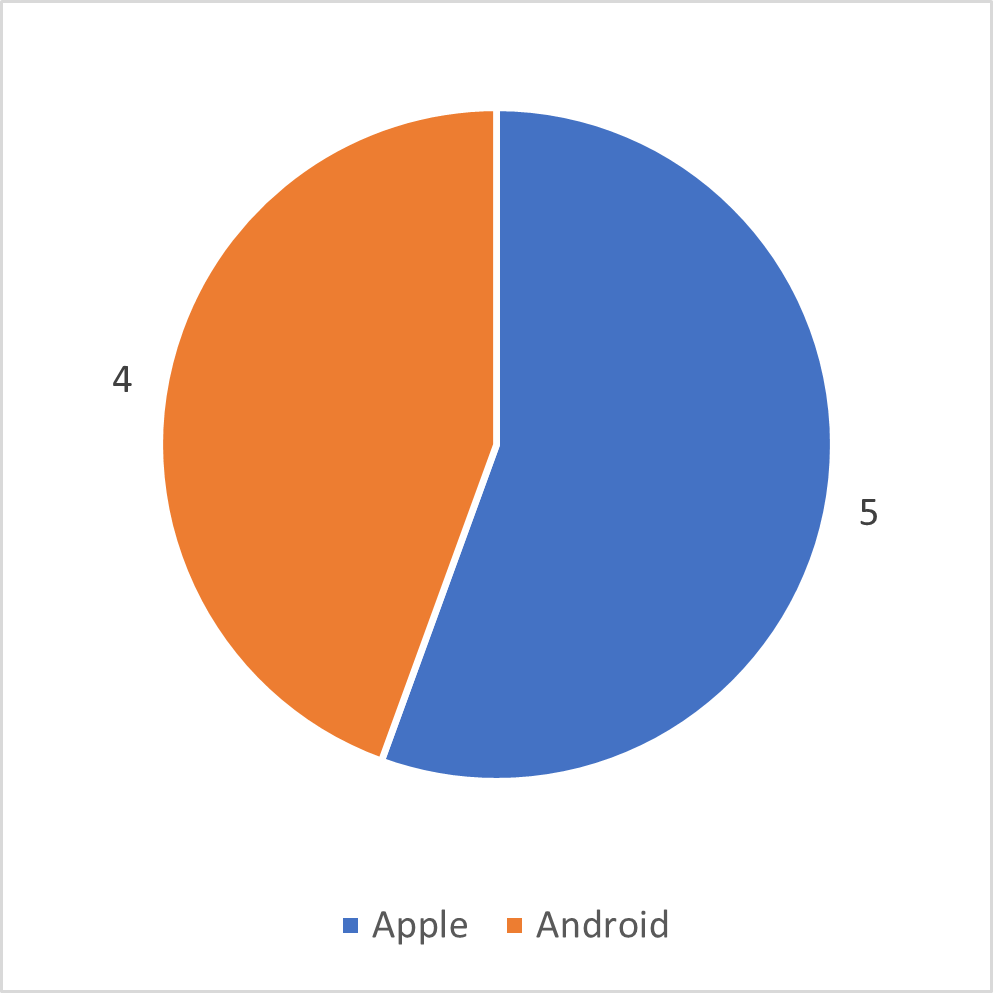
\includegraphics[width=0.5\linewidth]{Images/Phone-split.png}
    \caption{Study 2: Ratio of Android to IPhone users}
    \label{fig:phoneOS}
\end{figure}

\newpage
The Mosaic Cafe was the originally planned testing location, based on the range of products and lack of consistent labelling for food products. Figure \ref{fig:mosaic-use} breaks down whether participants were frequent shoppers at the cafe and whether nutritional value of the products was a major factor in their decisions of what to buy there. The inner ring shows the frequency that people visited the cafe, and the outer ring shows whether or not item nutrition impacts their decision to buy food there or not. Figure \ref{fig:health-concerns} shows the most common topics of concern reported by users. Participants mentioned multiple topics in their responses.  As a result, the numbers for our response analysis sum to numbers greater than participant totals. 

\begin{figure}[h]
    \centering
    \begin{subfigure}[b]{0.4\textwidth}
        \centering
         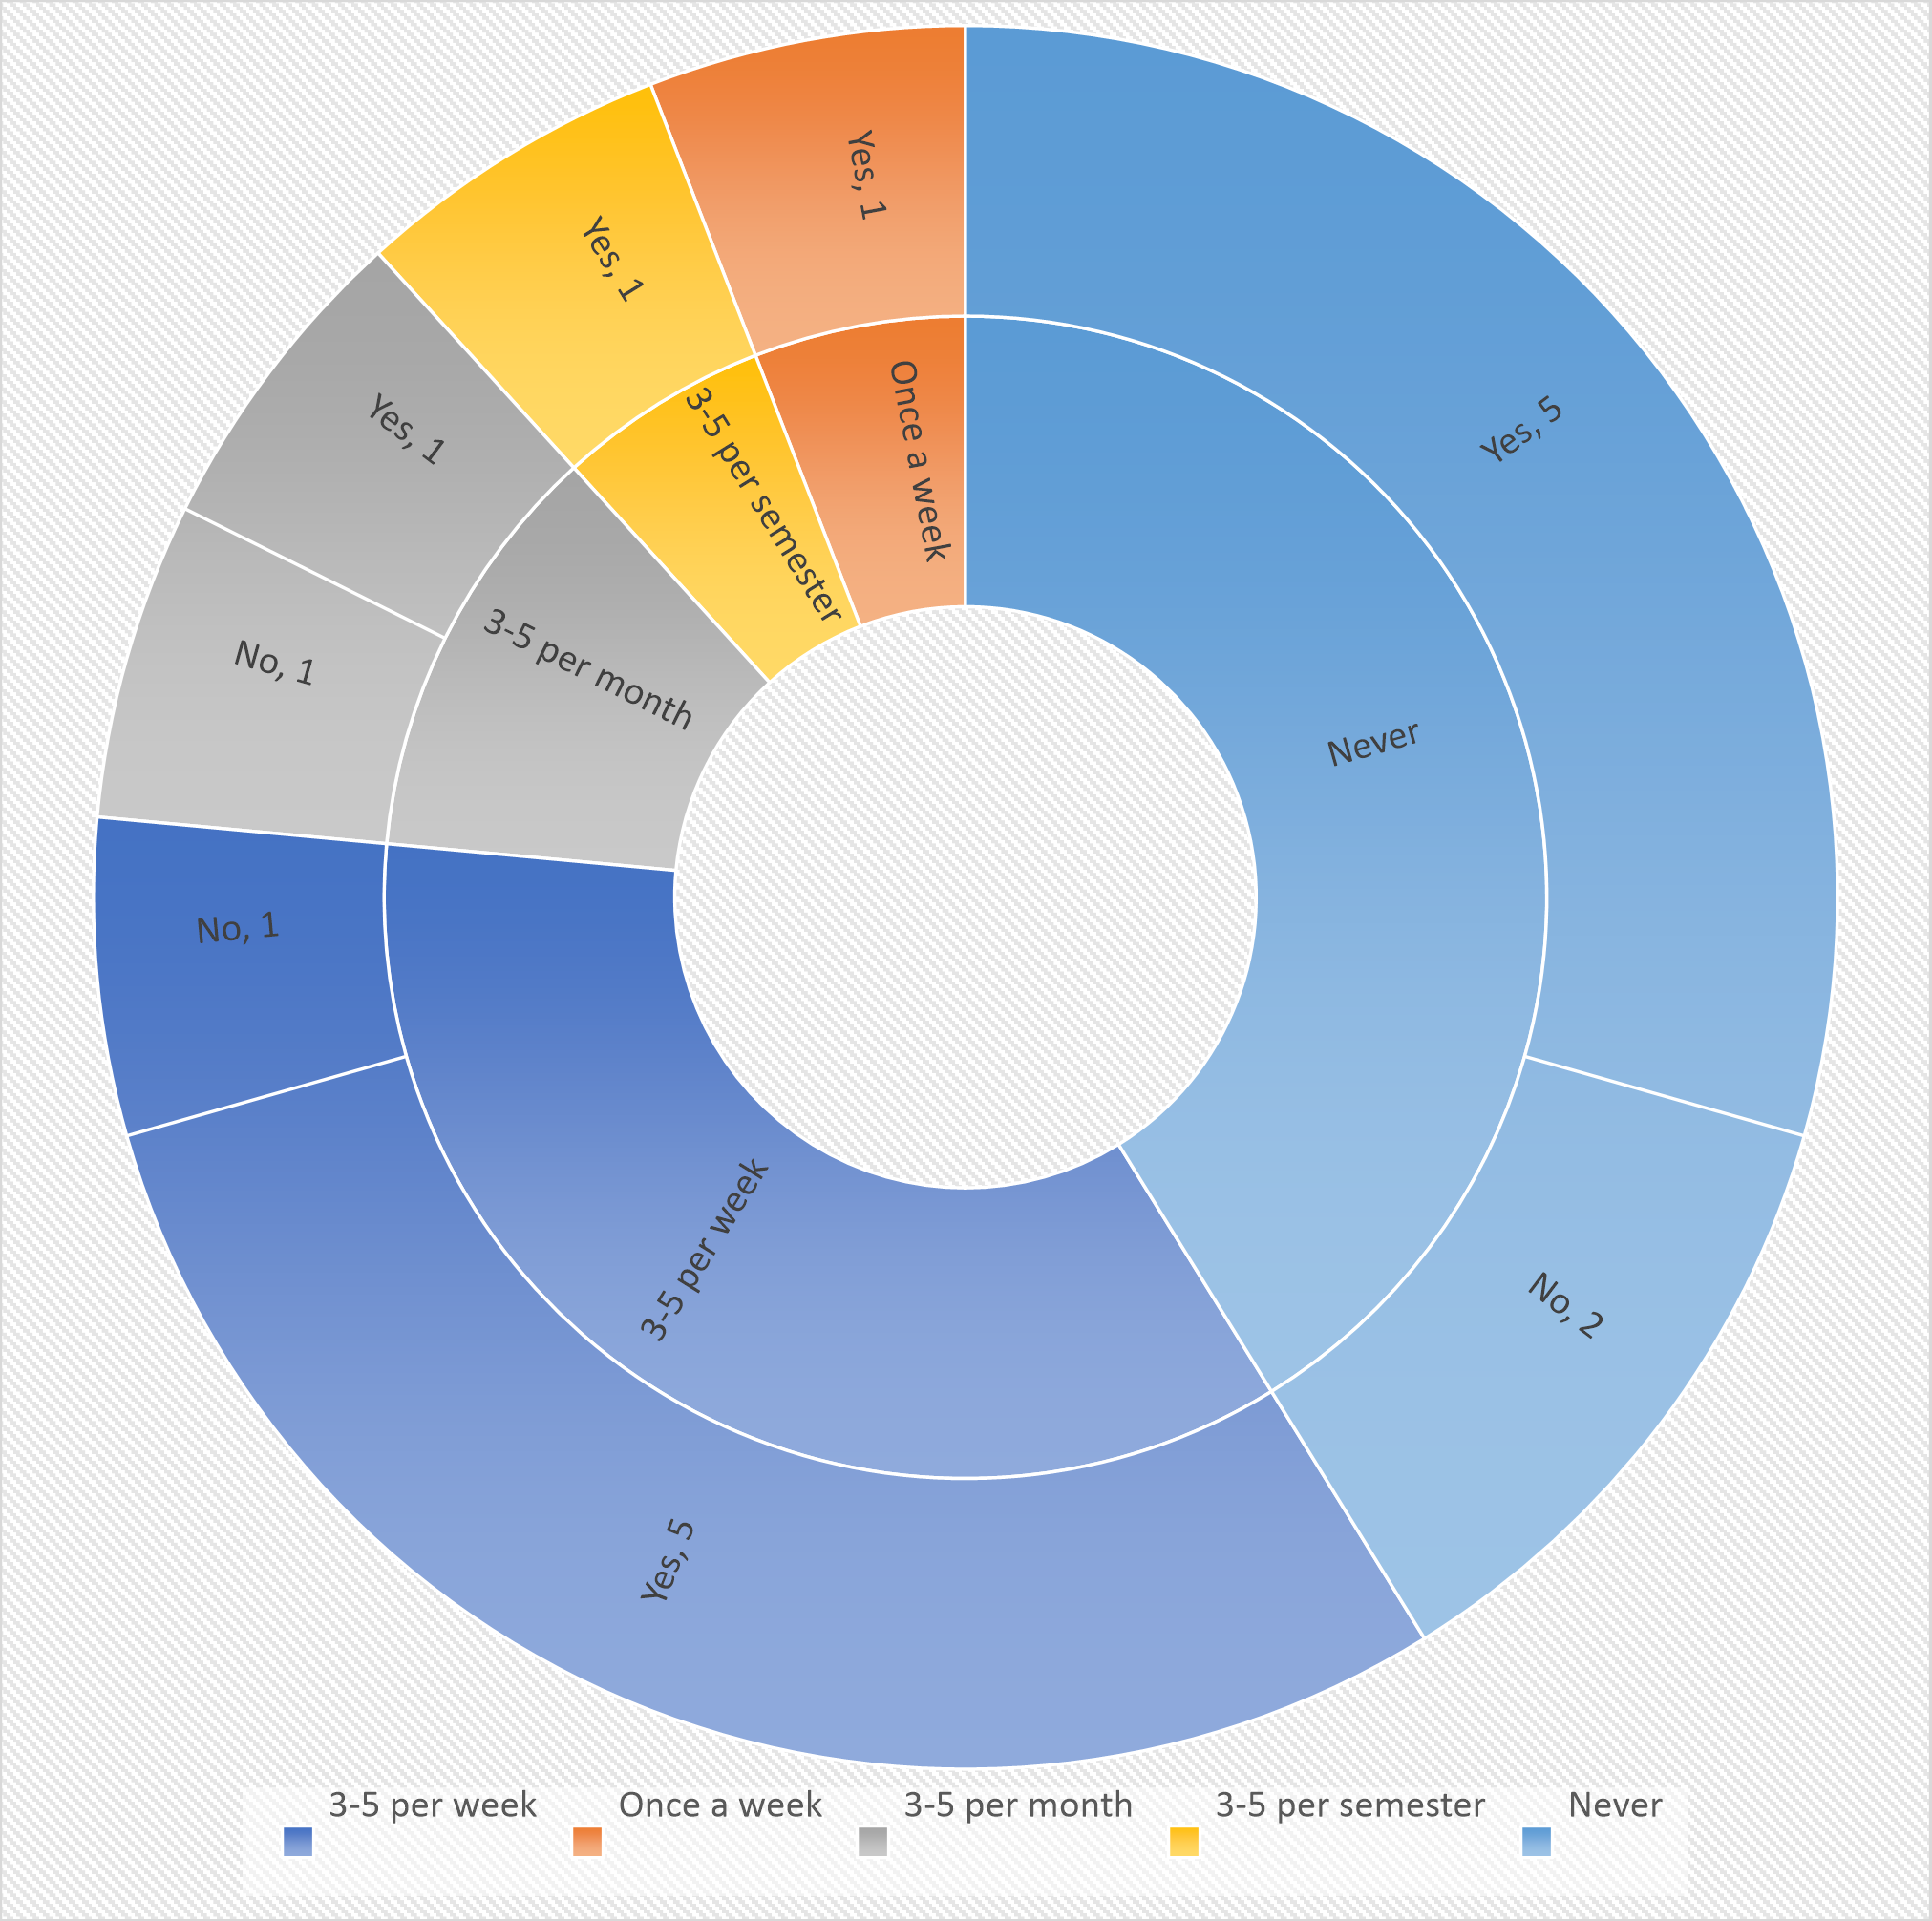
\includegraphics[scale=.38]{Images/Mosaic-use.png}
         \caption{Purchase frequency}
         \label{fig:mosaic-use}
    \end{subfigure}
    \begin{subfigure}[b]{0.4\textwidth}
        \centering
         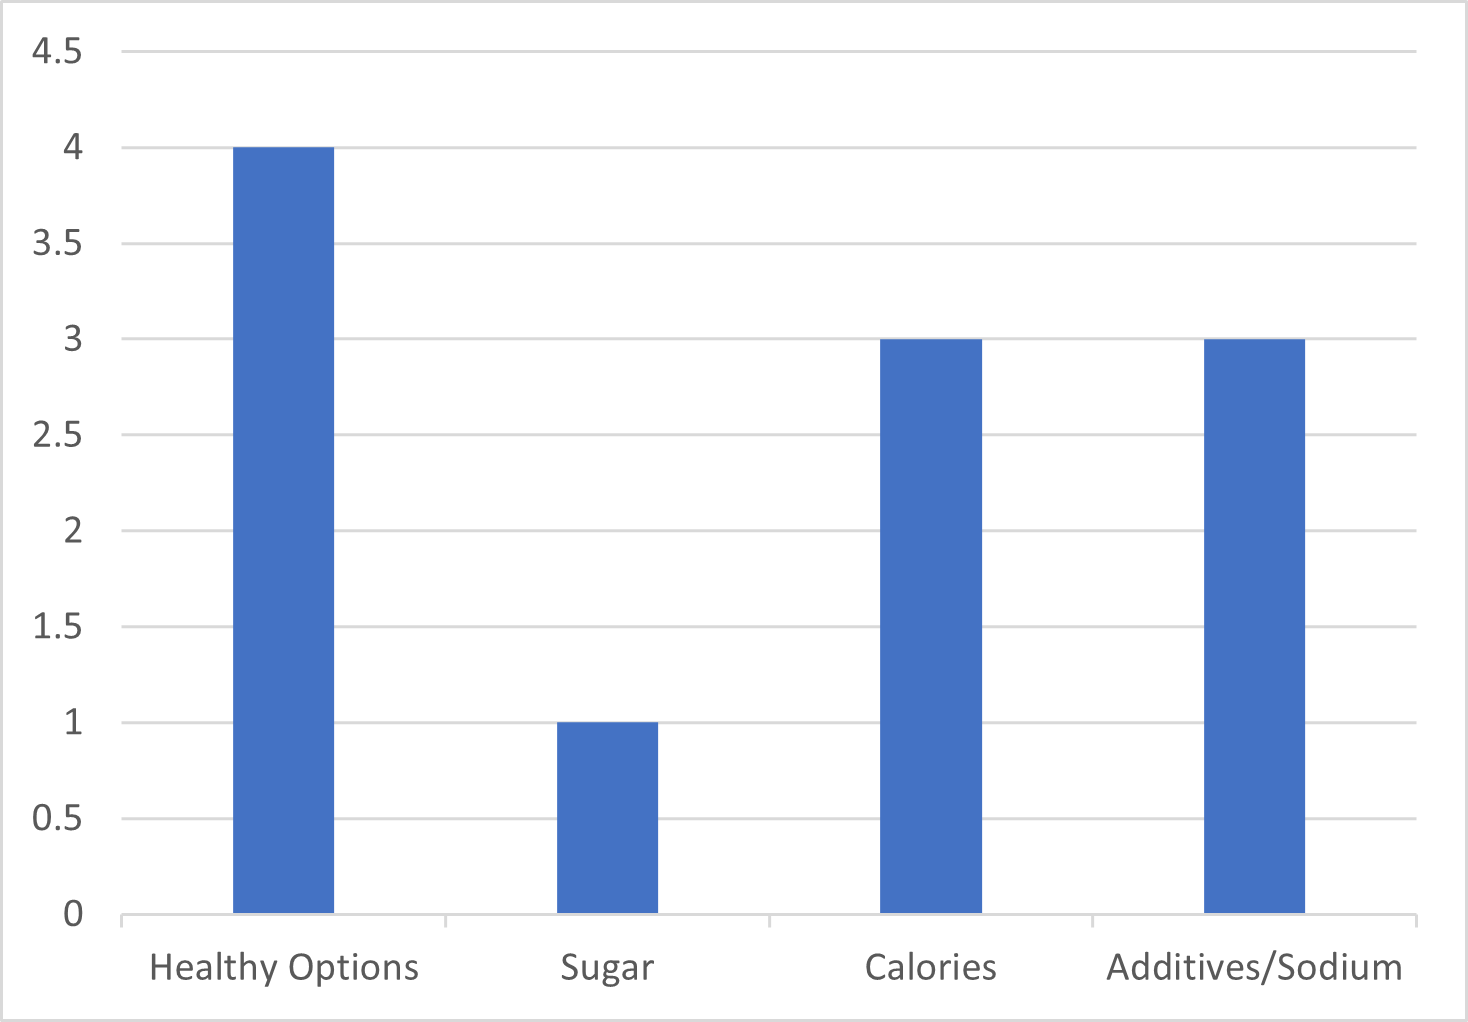
\includegraphics[width=\textwidth]{Images/Health-concerns.png}
         \caption{Health concerns expressed}
         \label{fig:health-concerns}
    \end{subfigure}
    \caption{Studies 1 \& 2: Relation between visits to Mosaic and nutrition concerns}
    \label{fig:}
\end{figure}

Participants reported whether they have any food allergies or eating restrictions. Across both studies, participants expressed a desire to exclude specific food types; one user selected "vegetarian," while multiple users requested the ability to exclude pork or specific meat types for health or moral reasons. Participants also reported difficulty reading nutrition labels, especially identifying ingredients and allergens when the font is small. Participants were also asked whether needing to pick up items to read the label was a concern and would they favor a tool to avoid that. Table \ref{tab:study1concerns} contains a breakdown of this information.
\begin{table}[h!]\centering
\caption{Studies 1 \& 2: Participant shopping concerns}\label{tab:study1concerns}
\ra{1.3}
\resizebox{\textwidth}{!}{%
\begin{tabular}{@{}lcllll@{}}
    \toprule
    \textbf{Study} & \textbf{\#} & \textbf{Allergies} & \textbf{Difficulty Reading}   & \textbf{Food Restrictions} & \textbf{Surface Contact} \\
    \midrule
    \multirow[t]{12}{.2\textwidth}{First Study}
      & 1 & No  & No & No              & Yes, mild concern      \\ 
      & 2 & No  & No & Yes, Vegetarian & Yes                    \\ 
      & 3 & No  & No & No              & No                     \\ 
      & 4 & No  & No & Yes, Kosher     & No                     \\ 
      & 5 & No  & No & No              & No                     \\ 
      & 6 & No  & No & No              & Yes, minimize touching \\ 
      & 7 & No  & No & No              & No                     \\ 
      & 8 & No  & No & No              & No                     \\ 
      & 9 & No  & No & No              & Yes, minimize touching \\ 
      & 10 & Yes & Yes, Visually Impaired & Yes, No red meat, low Calories and Sodium & Yes \\ 
      & 11 & Yes, Mushrooms & Yes, Small print hard to read & Yes, Additives & Yes \\ 
      & 12 & No & No & No               & Yes, pandemic concern  \\ 
    \\
    \multirow[t]{4}{.2\textwidth}{Second Study}
      & 1 & No & No & No               & Yes, germs and dirt    \\ 
      & 2 & No & No & No               & No                     \\ 
      & 3 & No & No & No               & Yes, spreading germs   \\ 
      & 4 & No & No & No               & No                     \\ 
    \bottomrule
\end{tabular}%
}
\end{table}


\section{NASA Task Load Index}
\subsection{First User Study}
The first step for processing and analyzing the results of the NASA TLX is to find the averages for each workload measure. Table \ref{tab:tlx-definitions} lists the different workload measures and what aspects they represent. The results for the first user tests are in Table \ref{tab:workloads}.

\begin{table}[h!]\centering
\caption{Study 1: TLX workload factor definitions and relevance}\label{tab:tlx-definitions}
\ra{1.3}
    \begin{tabular}{@{}l>{\raggedright\arraybackslash}p{\dimexpr 0.37\linewidth-2\tabcolsep}>{\raggedright\arraybackslash}p{\dimexpr 0.37\linewidth-2\tabcolsep}@{}}
    \toprule
        \textbf{Category} & \textbf{Definition} &   \textbf{App Relevance}  \\
    \midrule
        Mental Demand (MD)  &   How mentally demanding was the task?    &   App lacked features and had severe issues with the item locator, leading to incorrect behavior \\ 
        Physical Demand (PD)    &   How physically demanding was the task?  &   Users needed to walk around the area; The phone needed to be moved around the space \\
        Temporal Demand (TD)    &   How hurried or rushed was the pace of the task? &   There was a 10 minute time limit \\
        Performance (P) &   How successful were you in accomplishing what you were asked to do? &   Users were asked to try features at their own rate \\
        Effort (EF) &   How hard did you have to work to accomplish your level of performance? &    Tasks included moving around and looking at items   \\
        Frustration (FR)    &   How insecure, discouraged, irritated, stressed, and annoyed were you?    &   There were several technical issues in version 1 \\
    \bottomrule
    \end{tabular}%
\end{table}

\begin{table}[h!]\centering
\caption{Study 1: TLX workload measures}\label{tab:workloads}
\ra{1.2}
    \begin{tabular}{@{}crS@{}}
        \toprule
            \textbf{Category} & \textbf{Total} & \textbf{Average} \\
        \midrule
            E   &  1020 & 92.727 \\
            FR  &   810 & 73.636 \\ 
            MD  &   430 & 39.09  \\ 
            P   &   730 & 66.364 \\ 
            PD  &   500 & 45.455 \\ 
            TD  &   120 & 10.909 \\
        \cmidrule{1-3}
            Average of WWL & \multicolumn{2}{c}{20.06} \\
        \bottomrule
    \end{tabular}
\end{table}
The closer to zero the score is, the less impact that workload factor has on the overall experience. Effort (E) has the greatest score, closely followed by Frustration (FR). This lines up well with the many comments from participants on the many technical difficulties and issues in the original version of the app. 
WebXR seems to have significant difficulty identifying surfaces and depth when environment colors are similar. Most of the surfaces and spaces at the University, including the lab and the classrooms, feature white desks with white walls and grey floors. Issues resulting from this WebXR behavior included markers placed too far or too close to the camera, and a significant amount of waving the phone around to detect the space. 
The augmentation menus in the first version of the app were locked to match whatever rotation the phone was in when the \acrshort{ar} experience was first initiated, resulting in menus facing away from users and requiring people to move in order to read them. Users needed multiple attempts to get the object location to work correctly, and even then the markers weren't aligned properly most of the time. The increased requirements for moving the device around likely led to a moderately high score for Physical Demand (PD).

These and other significant issues stemming from flaws in the application implementation caused multiple participants to comment on how they felt disappointed they couldn't fully experience the described concept. We attribute the relatively high average score for Performance (P) to a combination of this feeling of failure on the part of the participant combined with many performance issues of the app. P is mainly intended to be a measure of the user's satisfaction with their own performance, but it's possible that this wasn't clear enough to participants.

Mental Demand (MD) and Temporal Demand (TD) are comparatively low. The app lacked many of the features that require user interaction, requiring minimal learning before use. Most participants finished long before the 10-minute time limit, and no one needed to be encouraged to finish up, leading to a low TD score. There was a significant time delay before the app started to properly place the markers in the space; most participants complained about the delay, but the actual time pressure wasn't greatly affected. 

Only judging the individual scores is not sufficient, we also needed to verify whether any of the workload factors were positively or negatively correlated, and whether the other factors can be used to predict the score for E. Table \ref{tab:correlation} shows the Pearson Correlation values for each of the workload scores.
\begin{table}[h]\centering
\caption{Study 1: Pearson correlation matrix}\label{tab:correlation}
\ra{1.2}
    \begin{tabular}{@{}c *{6}{S[table-format=1.4]} @{}}
    \toprule
            &   {\textbf{E}}  &   {\textbf{FR}} &   {\textbf{MD}} &   {\textbf{P}}  &   {\textbf{PD}} &   {\textbf{TD}} \\ 
    \midrule
        \textbf{E}  &   1.0000  &   0.2924  &   0.2013  &   0.2993  &    0.0865 &   0.4946  \\
        \textbf{FR} &   0.2924  &   1.0000  &   0.0136  &   -0.031  & \B 0.6466 &   0   \\
        \textbf{MD} &   0.2013  &   0.0136  &   1.000   &   0.1903  &   -0.1789 &   -0.1263 \\
        \textbf{P}  &   0.2993  &   -0.031  &   0.1903  &   1.000   &   -0.079  &   0.5407  \\        
        \textbf{PD} &   0.0865  & \B 0.6466 &   -0.1789 &   -0.079  &   1.000   &   -0.3174 \\
        \textbf{TD} &   0.4946  &   0.0000  &   -0.1263 &   0.5407  &   -0.3174 &   1.000 \\
    \bottomrule
    \end{tabular}
\end{table}
The only workload factors that show significant correlation are \acrfull{pd} and \acrfull{fr}, with a strong (greater than .5) positive correlation of 0.646. This implies that as one increases, the other will as well. This lines up well with comments from participants during testing that the amount of movement required to get WebXR to properly recognize the space was one of the most frustrating parts. 

Before performing regression, we used priori power analysis to test the significance of the entire model. The power to test the entire model is low: 0.2315, hence with a larger sample size the regression model may become significant.

The highest scoring workload factor from Table \ref{tab:workloads} is E. If we treat this as the value we wish to minimize, an equation based on the other workload scores can be calculated. The Coefficients of Regression Significance test allows us to identify the coefficients for this equation from the values from Iteration 1 in Table \ref{tab:regression1}:
\begin{equation}
    \label{eqn:regression11}
    \hat{Y} = 11.4873 + 0.102X_1 + 0.5191X_2 - 0.2318X_3 + 0.4001X_4 + 4.5454X_5
\end{equation}

\begin{table}[h!]\centering
\caption{Study 1: Coefficients of Regression Significance Test}\label{tab:regression1}
\ra{1.2}
\resizebox{\textwidth}{!}{%
    \begin{tabular}{@{}l *{2}{S[table-format=2.4]} c *{4}{S[table-format=1.4]} @{}}
        \toprule
            \textbf{Model}  &   \multicolumn{2}{c}{\textbf{Unstandardized Coefficients}}    &   \phantom{abc} & \textbf{Standardized Coefficients}  &   \textbf{t-stat} &   \textbf{p-value}    &   \textbf{VIF}    \\
        \cmidrule{2-3} \cmidrule{5-5}
                            & {\textit{B}} & \textbf{{Std. Error}} && \textbf{{Beta}} & & & \\
        \midrule
            \textbf{Iteration 1} \\
            Constant            &  11.4873 &   53.4981 &&   0.0000 &   0.2147  &   0.8371    &           \\
            Frustration Level   &   0.102  &   0.5946  &&   0.0768 &   0.1716  &   0.8694    &    2.1399 \\ 
            Mental Demand       &   0.5191 &   0.4985  &&   0.3720 &   1.0413  &   0.3379    &    1.3647 \\ 
            Performance         &  -0.2318 &   0.7268  &&  -0.1293 &  -0.3189  &   0.7606    &    1.7575 \\ 
            Physical Demand     &   0.4001 &   0.6199  &&   0.3194 &   0.6455  &   0.5425    & \B 2.6191 \\ 
            Temporal Demand     &   4.5454 &   2.8864  &&   0.7129 &   1.5748  &   0.1664    &    2.1913 \\
            \textbf{Iteration 2} \\
            Constant            &  14.1362 &  47.5383  &&   0.0000 &   0.2974  &   0.7748    &           \\
            Mental Demand       &   0.5466 &   0.438   &&   0.3918 &   1.2481  &   0.2521    & 1.2231    \\
            Performance         &  -0.2653 &   0.6497  &&  -0.148  &  -0.4083  &   0.6953    & 1.6307    \\
            Physical Demand     &   0.4777 &   0.3937  &&   0.3814 &   1.2133  &   0.2644    & 1.2265    \\
            Temporal Demand     &   4.751  &   2.4371  &&   0.7451 &   1.9495  & \B 0.0922    & 1.8137    \\
            \textbf{Iteration 3} \\
            Constant            &   7.5863 &  42.3552  &&   0      &   0.1791  &   0.8623    &           \\
            Mental Demand       &   0.4843 &   0.3885  &&   0.3471 &   1.2464  &   0.2479    & 1.0744    \\ 
            Physical Demand     &   0.445  &   0.3648  &&   0.3552 &   1.2196  &   0.2573    & 1.1757    \\
            Temporal Demand     &   4.152  &   1.8419  &&   0.6512 &   2.2542  & \B 0.0542    & 1.1565    \\
            \textbf{Iteration 4} \\
            Constant            &  37.9027 &  35.2107  &&   0      &   1.0765  &   0.3097    &           \\ 
            Mental Demand       &   0.374  &   0.3879  &&   0.3471 &   0.964   &   0.3602    & 1.0162    \\
            Temporal Demand     &   3.3696 &   1.7728  &&   0.6512 &   1.9008  & \B 0.0898   & 1.0162    \\
            \textbf{Iteration 5} \\
            Constant            &  53.4615 &  31.1832  &&   0      &   1.0765  &   0.1172    &           \\
            Temporal Demand     &   3.1538 &   1.7523  &&   0.4946 &   1.9008  &   0.1021    & 1.0000    \\
        \bottomrule
    \end{tabular}%S
    }
\end{table}

The definition for equation \ref{eqn:regression11} is: \(\hat{Y} = E, X_1 = FR, X_2 = MD, X_3 = P, X_4 = PD, X_5 = TD\). The Variance Inflation Factor (VIF) indicates whether multicollinearity, the correlation between multiple independent variables, is likely to exist for each factor. The higher the value, the more inflated that coefficient is at a linear factor to other variables. Values above 2.50 indicate correlation may exist; values over 5.00 indicate high correlation. The only factor in Table \ref{eqn:regression11} with a VIF above 2.50 is Physical Demand.  To verify if PD was significant, we eliminated the factor with the highest p-score and repeated the analysis, as shown in Table \ref{tab:regression1}. Equation \ref{eqn:final-regression1} is the final result of iteration 4. TD is not significant in iteration 5.

Results of the multiple linear regression indicated that there was a moderate collective non-significant effect between the X1, X2, X3, X4, X5, and Y, \(F(1, 10) = 3.24, p = .102, R^2 = 0.24, R^2_{adj} = 0.17\).
\begin{equation}
    \label{eqn:final-regression1}
    \hat{Y} = 53.4615 + 3.1538X_5
\end{equation}

\filbreak
\subsection{Second User Study}
The second user study conducted only had 9 participants. This was the minimum number necessary to produce a valid result from regression testing; optimally we would need at least 12-14 participants. The process for analyzing the TLX data from Study 2 was the same as Study 1. Table \ref{tab:tlx-definitions2} contains descriptions of how each workload factor is relevant to system, while Table \ref{tab:workloads2} lists the sums, averages, and average WWL. 

\begin{table}[h]\centering
\caption{Study 2: TLX workload factor relevance }\label{tab:tlx-definitions2}
\ra{1.3}
    \begin{tabular}{@{}>{\raggedright\arraybackslash}p{\dimexpr 0.4\linewidth-2\tabcolsep}>{\raggedright\arraybackslash}p{\dimexpr 0.6\linewidth-2\tabcolsep}@{}}
        \toprule
            \textbf{Category}   &   \textbf{App Relevance}  \\
        \midrule
            Mental Demand (MD)      &   App only has two menus for user settings and searching; adding to home screen didn't always prompt   \\
            Physical Demand (PD)    &   Users needed to walk around the area and the phone needed to be moved around the space  \\
            Temporal Demand (TD)    &   There was a 10 minute time limit                   \\
            Performance (P)         &   Users were asked to try features at their own rate \\
            Effort (EF)             &   Tasks included moving around and looking at items  \\
            Frustration (FR)        &   Hitting the markers was imprecise, marker depth was often wrong, establishing marker locations was slow \\
        \bottomrule
    \end{tabular}%
\end{table}

\begin{table}[h]\centering
\caption{Study 2: TLX workload measures}\label{tab:workloads2}
\ra{1.2}
    \begin{tabular}{@{}c S[table-format=4.2] S[table-format=3.2] @{}}
        \toprule
            \textbf{Category}   &   \textbf{Total}  &   \textbf{Average}    \\
        \midrule
        E   &   \sisetup{round-precision = 2}  1470   & \sisetup{round-precision = 2}  \B 163.333    \\
        FR  &   \sisetup{round-precision = 2}  780    &  \sisetup{round-precision = 2}  86.667    \\
        MD  &    \sisetup{round-precision = 2}  450    &     \sisetup{round-precision = 2}  50         \\
        P   &   \sisetup{round-precision = 2}  1000    &    \sisetup{round-precision = 2}  111.111    \\ 
        PD  &    \sisetup{round-precision = 2}  460    &     \sisetup{round-precision = 2}  51.111    \\
        TD  &    \sisetup{round-precision = 2}  330    &     \sisetup{round-precision = 2}  36.667    \\
        \cmidrule{1-3}
        Average of WWL & \multicolumn{2}{c}{33.26} \\ 
        \bottomrule
    \end{tabular}
\end{table}
\filbreak
Like the first study, \acrfull{e} was the highest scoring workload, reflecting the increased number of user interactions and continued difficulties with marker placement. Multiple users complained that the length of time between entering \acrshort{ar} and first marker placement was too long, and that they weren't sure the app was working as a result. Successfully using the system required a significant amount of patience and willingness to learn and work with the system's quirks. The second highest scoring measure was \acrfull{p}, displacing \acrfull{fr} from the first study. The issues that led to the high frustration scores in the first study were still present in the second, but the overall experience was improved enough that participants cared less about the technical issues and more about the system's usefulness as a tool. Multiple users reported during the trials that they really liked the concept and the execution but were disappointed that they were unable to fully use the system.

\acrfull{fr} was the third highest scored workload measure. Multiple issues present in the first version persisted into the second, including marker placement, environment tracking speed, and user interactability with augmentations. Markers convey information better at a glance in the second version, but many users found them difficult to tap on. The app was also prone to random instability, especially if the screen changed sizes from rotation or opening the keyboard. Users also dealt with an issue that would cause the screen to rapidly flash white, requiring a refresh. 

\acrfull{md} and \acrfull{pd} had nearly equivalent scores, with a slight increase from the first study. The user interface was nearly feature complete, with a simple to use navigation system; most options were well labeled or self-explanatory. One participant commented that labels or tooltips for the mode selector should be added; others suggested methods to help reduce uncertainty around different UI elements. The physical demand was reduced from the first version in two ways:
\begin{enumerate}
    \item Menus open facing the user, eliminating unnecessary steps
    \item Item location and marker placement speed and accuracy improved, reducing resets
\end{enumerate}
These improvements eliminated most of the wasted movements required to place the markers in the first version, and all the participants that tried both versions commented on the increase in usefulness of the system for these and other reasons.

\acrfull{td} remained the lowest factor, despite the number of suggested tasks increasing and the time limit remaining at 10 minutes. None of the participants reached the time limit, and the improvements listed above helped ensure users needed to wait less time for marker placement and interactability compared to the first version. Depth detection issues and programming errors led to a degraded user experience in other areas.

Correlation analysis for the workload factors followed the same process as the first study. Table \ref{tab:correlation2} shows the correlation values for each pair of workload measures. \acrfull{pd} and \acrfull{e} have a strong positive correlation. This finding is supported by the comments from participants during testing and in their responses that having to wave their phone around or move it away to "reset" the view were both too much work compared to the ideal: point the phone at the item and get instant feedback.

\begin{table}[h]\centering
\caption{Study 2: Pearson correlation matrix}\label{tab:correlation2}
\ra{1.2}
    \begin{tabular}{@{}c *{6}{S[table-format=1.4]} @{}}
        \toprule
                 & {\textbf{E}} & {\textbf{FR}} & {\textbf{MD}} & {\textbf{P}} & {\textbf{PD}} & {\textbf{TD}}\\
        \midrule
            \textbf{E}  &   1.000   &   -0.077  &   0.1767  &   -0.4936 & \B 0.821   &   0.0912  \\
            \textbf{FR} &  -0.077   &    1.000  &   0.2277  &    0.0815 &  -0.275   &   -0.1453 \\
            \textbf{MD} &   0.1767  &    0.2277 &   1.000   &    0.1603 &   0.217   &   -0.4473 \\
            \textbf{P}  &  -0.4936  &    0.0815 &   0.1603  &    1.000  &  -0.231   &   -0.105  \\
            \textbf{PD} & \B 0.821   &   -0.275  &   0.217   &   -0.231  &   1.000   &   -0.2502 \\
            \textbf{TD} &   0.0912  &   -0.1453 &  -0.4473  &   -0.105  &  -0.2502  &    1.000  \\ 
        \bottomrule
    \end{tabular}
\end{table}

In the first study, we lacked the participant data to perform ANOVA analysis of the significance of the regression model. More participants and better procedures to inform and instruct them may have reduced the issues with multicollinearity during analysis by reducing confusion over the workload definitions and relevance. The results of analysis for the second study are in Table \ref{tab:anova2}. 
\begin{table}[h]\centering
\caption{Study 2: ANOVA test for model significance}\label{tab:anova2}
\ra{1.2}
    \begin{tabular}{@{}lc*{2}{S[table-format=5.4]}*{2}{S[table-format=2.4]}@{}}
        \toprule
            \textbf{Source} &   \textbf{DoF}    &   \textbf{Sum of Squares} &   \textbf{Mean Square}    &   \textbf{F-stat} &   \textbf{P-value}    \\
        \midrule
            \textbf{Regression} &   1   &   88560.94238 &   88560.94238     &   14.471061   & \B 0.00667915  \\
            \textbf{Residual}   &   7   &   42839.05762 &    6119.865374    &               &                \\
            \textbf{Total}      &   8   &  131400       &   16425           &               &                \\
        \bottomrule
    \end{tabular}%
\end{table}
The mean-square values for the residual and regression both indicate the regression is highly unlikely to be significant. Despite this, the p-value strongly indicates the model is significant (\(\textit{p}\leq.01\)). We consider this evidence that the improvements to the system have increased our ability to assess areas of needed improvement. More participants are needed to verify the significance and validity of the model for more difficult use cases.

Effort is the highest scoring workload factor according to Table \ref{tab:workloads2}, unchanged from the first study. Table \ref{tab:regression2} covers the steps in verifying which coefficients of regression remain significant for the equation to predict E. Unlike the first study, no multicollinearity was present between the factors (The VIF values were all under 2.5). The power to test the model, calculated before regression (Priori Power), is low at 0.1739, but we choose to reject \(H_0\), as the power to prove that each predictor is significant is always lower than the power to test the entire model.

The definitions for the regression equation \ref{eqn:regression2} remained the same: \(\hat{Y} = E, X_1 = FR, X_2 = MD, X_3 = P, X_4 = PD, X_5 = TD\). Both coefficients in the final iteration were significant, meaning the model has some value for predicting \acrlong{e} based on the final equation for the regression model is below:
\begin{equation}
    \label{eqn:regression2}
    \hat{Y} = 108.972467 + 1.063582X_4
\end{equation}
Results of the multiple linear regression indicated that there was a very strong collective significant effect between the X1, X2, X3, X4, X5, and Y, \(F(1, 7) = 14.47, p = .007, R^2 = 0.67, R^2_{adj} = 0.63\).

\newpage
\begin{table}[h!]\centering
\caption{Study 2: Coefficients of Regression Significance Test}\label{tab:regression2}
\ra{1.2}
    \resizebox{\textwidth}{!}{
        \begin{tabular}{@{}l *{2}{S[table-format=2.4]} c *{4}{S[table-format=1.4]} @{}}
            \toprule
                \textbf{Model}  &   \multicolumn{2}{c}{\textbf{Unstandardized Coefficients}}    &   \phantom{abc} & \textbf{Standardized Coefficients}  &   \textbf{t-stat} &   \textbf{p-value}    &   \textbf{VIF}    \\
            \cmidrule{2-3} \cmidrule{5-5}
                                & {\textit{B}} & \textbf{{Std. Error}} && \textbf{{Beta}} & & & \\
            \midrule
                Iteration 1 \\
                Constant            &  59.638309    &   75.813473   &&   0      &   0.7866  &   0.4889  &           \\
                Frustration Level   &   0.236145    &   0.22431     &&   0.2054 &   1.053   &   0.3698  &   1.2158  \\
                Mental Demand       &   0.630871    &   0.834647    &&   0.1576 &   0.7559  &   0.5047  &   1.3887  \\
                Performance         &  -0.535334    &   0.340579    &&  -0.295  &  -1.5718  &   0.214   &   1.1248  \\
                Physical Demand     &   1.126737    &   0.266747    &&   0.8697 &   4.224   &   0.0243  &   1.3542  \\
                Temporal Demand     &   1.461229    &   0.785784    &&   0.3781 &   1.8596  &   0.1599  &   1.3209  \\
                Iteration 2 \\
                Constant            &  87.6573      &  62.4886      &&   0      &   1.4028  &   0.2333  &           \\
                Frustration Level   &   0.2777      &   0.2055      &&   0.2415 &   1.3513  &   0.248   &    1.1429 \\ Performance         &  -0.4897      &   0.3167      &&  -0.2698 &  -1.5461  &   0.197   &    1.089  \\
                Physical Demand     &   1.1741      &   0.245       &&   0.9063 &   4.7927  &   0.0087  &    1.2794 \\
                Temporal Demand     &   1.2547      &   0.6961      &&   0.3247 &   1.8023  &   0.1458  &    1.1612 \\
                Iteration 3 \\
                Constant            & 126.0916      &  60.0603      &&  0      &   2.0994  &   0.0898  &           \\
                Performance         &  -0.4988      &   0.3418      && -0.2748 &  -1.4595  &   0.2043  &    1.0889 \\
                Physical Demand     &   1.0684      &   0.2506      &&   0.8247 &   4.2635  &   0.008   &    1.1488 \\
                Temporal Demand     &   1.038       &   0.7312      &&   0.2686 &   1.4195  &   0.215   &    1.0996 \\
                Iteration 4 \\
                Constant            & 178.6246      &  51.14995     &&   0      &   3.4922  &   0.0129  &           \\
                Performance         &  -0.5827      &   0.364       &&  -0.2748 &  -1.6007  &   0.1606  &    1.0564 \\
                Physical Demand     &   0.9675      &   0.2598      &&   0.8247 &   3.7236  &   0.0098  &    1.0564 \\
                Iteration 5 \\
                Constant            & 108.9725      &  29.7354      &&   0      &   3.6647  &   0.008   &           \\
                Physical Demand     &   1.0636      &   0.2796      &&   0.8209 &   3.8041  &   0.0067  &    1      \\
            \bottomrule    
        \end{tabular}%
    }
\end{table}
\pagebreak
\section{System Usability Scale}
Workload is an important measure of how a system affects the users of that system, but the \acrfull{sus} score helps to analyze how helpful and useful the system is to those same users. Unlike the TLX, scores from the SUS can be compared against different types of scales depending on the score use case. The SUS questionnaire is short and simple to score and can be effectively used for nearly any system. Figure \ref{fig:sus-plot} shows a boxplot of the data in Table \ref{tab:sus-scores}. Individual scores should be ignored for analysis, we plotted them anyway to show how they were distributed.

\begin{figure}[h]
    \centering
    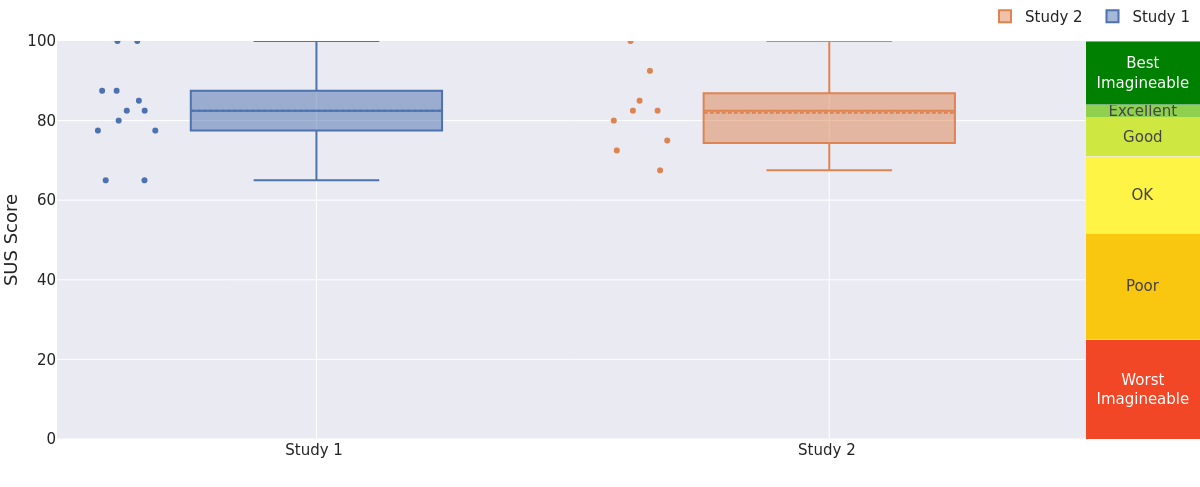
\includegraphics[width=\textwidth]{Images/main_plot.png}
    \caption{Studies 1 \& 2: SUS distribution and adjective ranking plot}
    \label{fig:sus-plot}
\end{figure}

\begin{table}[h]\centering
\caption{Studies 1 \& 2: SUS statistics}\label{tab:sus-scores}
\ra{1.2}
    \resizebox{\textwidth}{!}{%
        \begin{tabular}{@{}l *{7}{S[table-format=3.2]} l@{}}
            \toprule
                \textbf{Variable}   &   \textbf{SUS Score (mean)}   &   \textbf{Std. Dev.}  &   \textbf{Min}    &   \textbf{Max}    &   \textbf{1st Quartile}   &   \textbf{Median} &   \textbf{3rd Quartile}   &   \textbf{Adjective}   \\
            \midrule
                Study 1 &  \sisetup{round-precision = 2} 82.5    &  \sisetup{round-precision = 2} 10.56   & \sisetup{round-precision = 2} 65   & \sisetup{round-precision = 2}  100 & \sisetup{round-precision = 2}  77.5    & \sisetup{round-precision = 2}  82.5    & \sisetup{round-precision = 2}  87.5    &   Excellent \\ 
                Study 2 &  \sisetup{round-precision = 2} 81.94   &  \sisetup{round-precision = 2}  9.41   & \sisetup{round-precision = 2} 67.5 & \sisetup{round-precision = 2}  100 & \sisetup{round-precision = 2}  73.75   & \sisetup{round-precision = 2}  82.5    & \sisetup{round-precision = 2}  88.75   &   Excellent \\
            \bottomrule
        \end{tabular}%
    }
\end{table}

\filbreak
Figure \ref{fig:conclusiveness} plots the conclusiveness percentage, or how reliable the score for each study is in accurately representing user sentiment and preference. We had an adequate number of participants for our first study, with 12 people being just enough to have 100\% conclusiveness. The second study had 9 participants, only reaching 75\% conclusiveness.

\begin{figure}[h!]
    \centering
    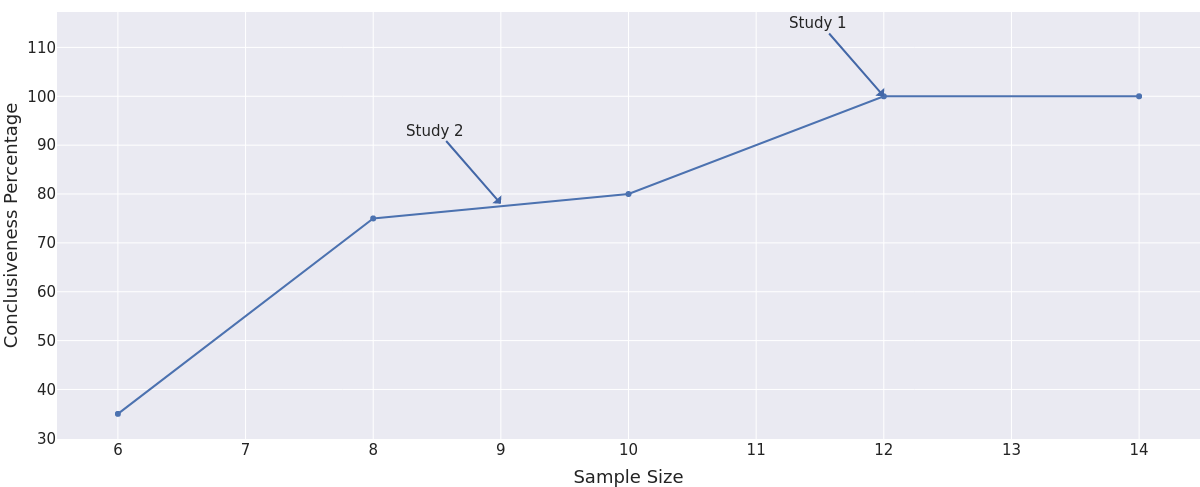
\includegraphics[width=\textwidth]{Images/conclusiveness_plot.png}
    \caption{Studies 1 \& 2: SUS conclusiveness graph}
    \label{fig:conclusiveness}
\end{figure}

\section{Post-survey Analysis}
The pre-survey analysis section above combines the results from the first and second studies, as the surveys were relatively similar and the overlap between the sample groups was significant (75\%). We take a similar approach for the post-surveys, comparing the key themes and words from each response to the shared questions between the first and second studies. Each question is addressed in order based on the surveys. 

\subsection{Study 2 Question Analysis}
\begin{enumerate}
    \item[] \textbf{Question: } Did you participate in the user study for the first version? If you answered yes to the previous question, what are your impressions of the new version, and does it address some of the concerns from the first test?
    \filbreak
    \item[] \textbf{Response Analysis: } More than half of the participants in the second study (66\%) had participated in the first and were able to comment on the improvements and ongoing issues for the system. Comments were mostly enthusiastic and impressed with the improvements. Many participants expressed concerns about the tracking and marker system still lacking accuracy, and there were new issues involving markers placed too far from the physical item and camera.
\end{enumerate}

\begin{enumerate}
    \item[] \textbf{Question: } Did you have any major issues?
    \item[] \textbf{Response Analysis: }  Figure \ref{fig:major-issues} shows what issues caused participants the most dissatisfaction. Speed and accuracy were the two major issues for the first version. Both improved in the second version but depth sensing problems led to a range of other issues including augmentations with incorrect scaling.
\end{enumerate}

\begin{figure}[h]
    \centering
    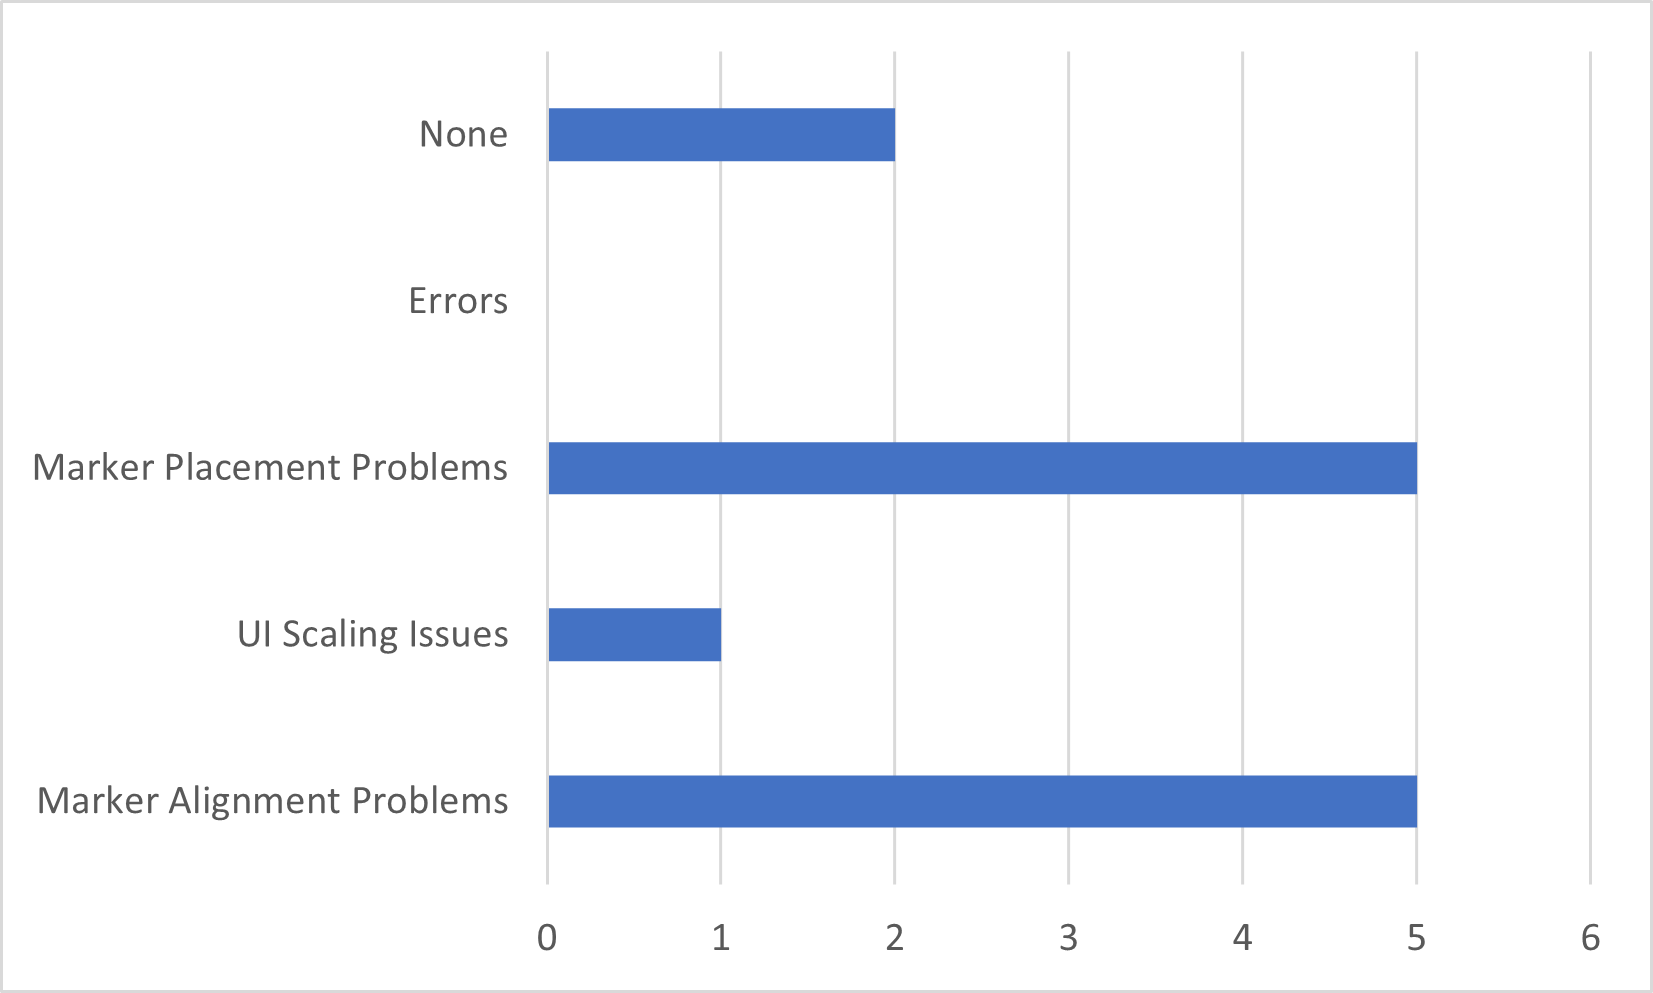
\includegraphics[width=.75\textwidth]{Images/major-issues.png}
    \caption{Study 2: User reported issues}
    \label{fig:major-issues}
\end{figure}

\filbreak
\subsection{Studies 1 \& 2 Question Analysis}
\begin{enumerate}
    \item[] \textbf{Question: } Did use of the "Item-FindAR" app improve the simulated shopping experience? How does having an \acrshort{ar} shopping tool compare to/change the experience of traditional shopping?
    \item[] \textbf{Response Analysis: } Participant responses and reactions to the system prototypes and overall concept were overwhelmingly positive. Figure \ref{fig:experience} shows the yes/no results of the first part of the question, a nearly unanimous "yes" across both studies. This aligns well with the reactions and opinions expressed during the trials, and the short responses to the latter half of the question. The thematic and tonal analysis of those responses are shown in Figure \ref{fig:experience-themes}.
\end{enumerate}

\begin{figure}[h]
    \centering
    \begin{subfigure}[]{.45\textwidth}
        \centering
        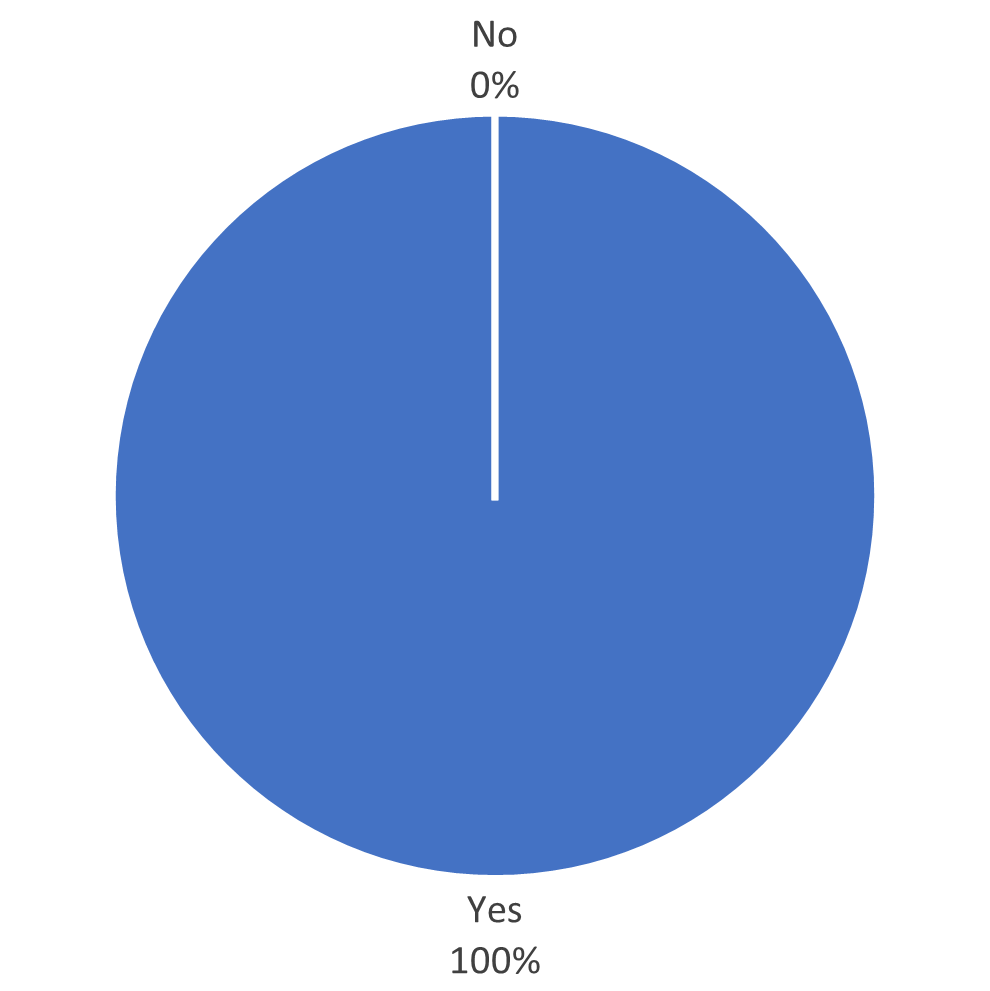
\includegraphics[width=\textwidth]{Images/experience study 1.png}
        \caption{First Study}
    \end{subfigure}
    \begin{subfigure}[]{.45\textwidth}
        \centering
        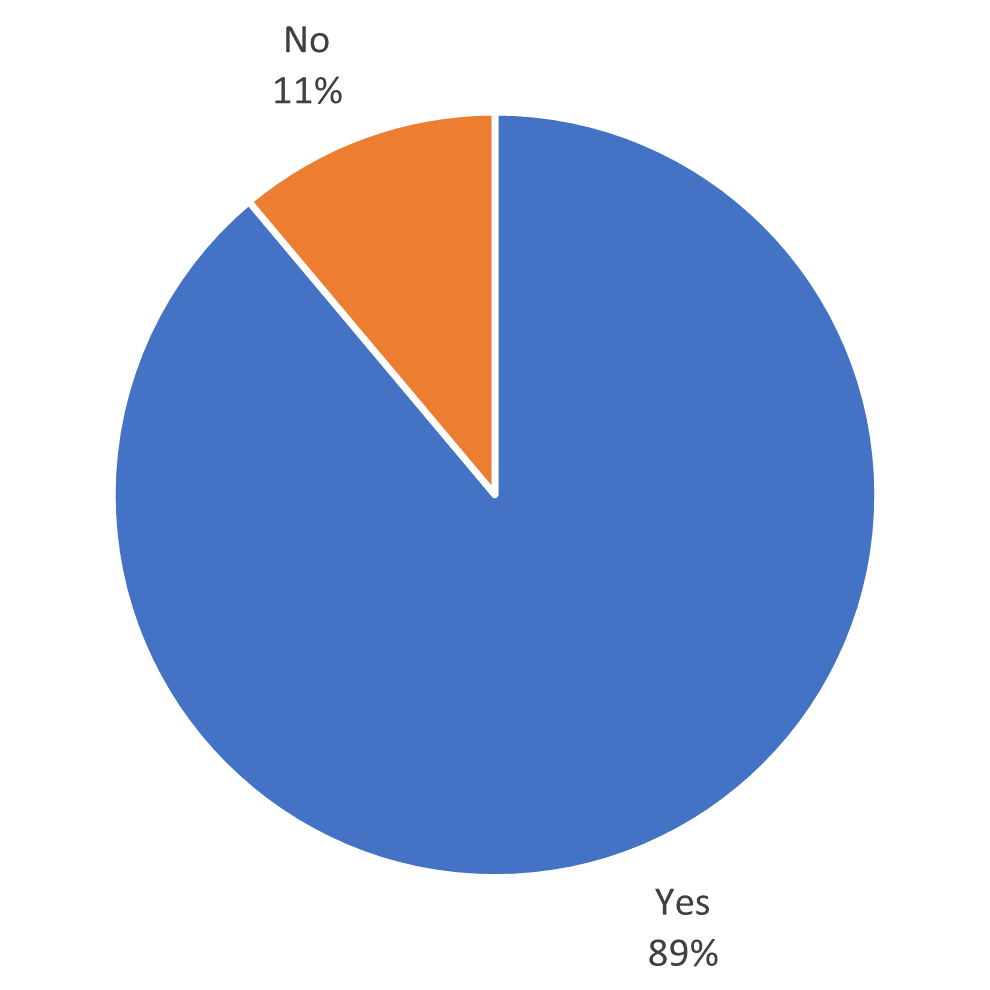
\includegraphics[width=\textwidth]{Images/experience study 2.png}
        \caption{Second Study}
    \end{subfigure}
    \caption{Studies 1 \& 2: Did the Item-FindAR system improve the shopping experience?}
    \label{fig:experience}
\end{figure}

\begin{figure}[h!]
    \centering
    \begin{subfigure}[]{.45\textwidth}
        \centering
        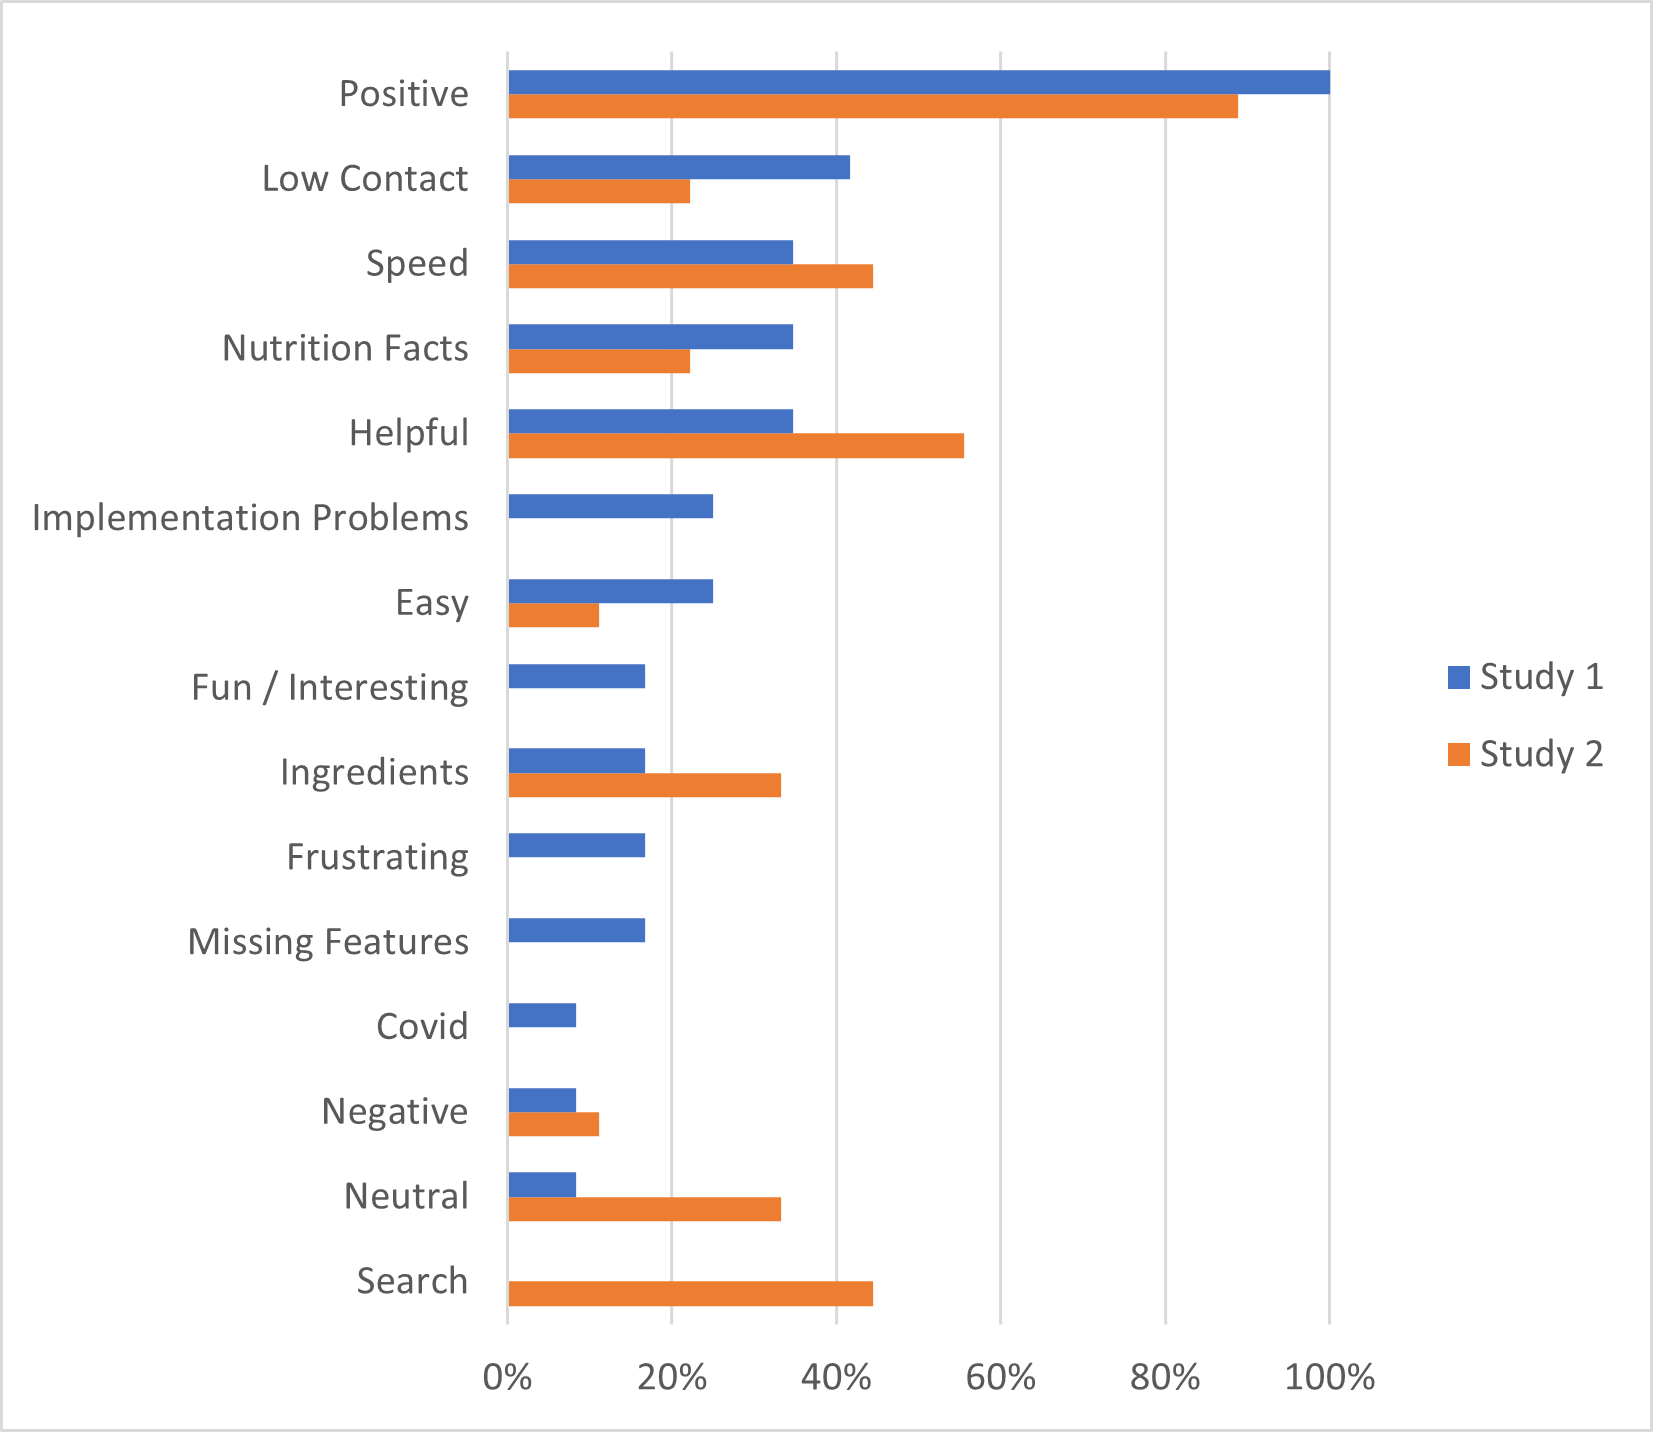
\includegraphics[width=\textwidth]{Images/experience themes study 1.png}
        \caption{Themes sorted by Study 1 percentages}
        \label{fig:exp-themes-study1}
    \end{subfigure}
    \begin{subfigure}[]{.45\textwidth}
        \centering
        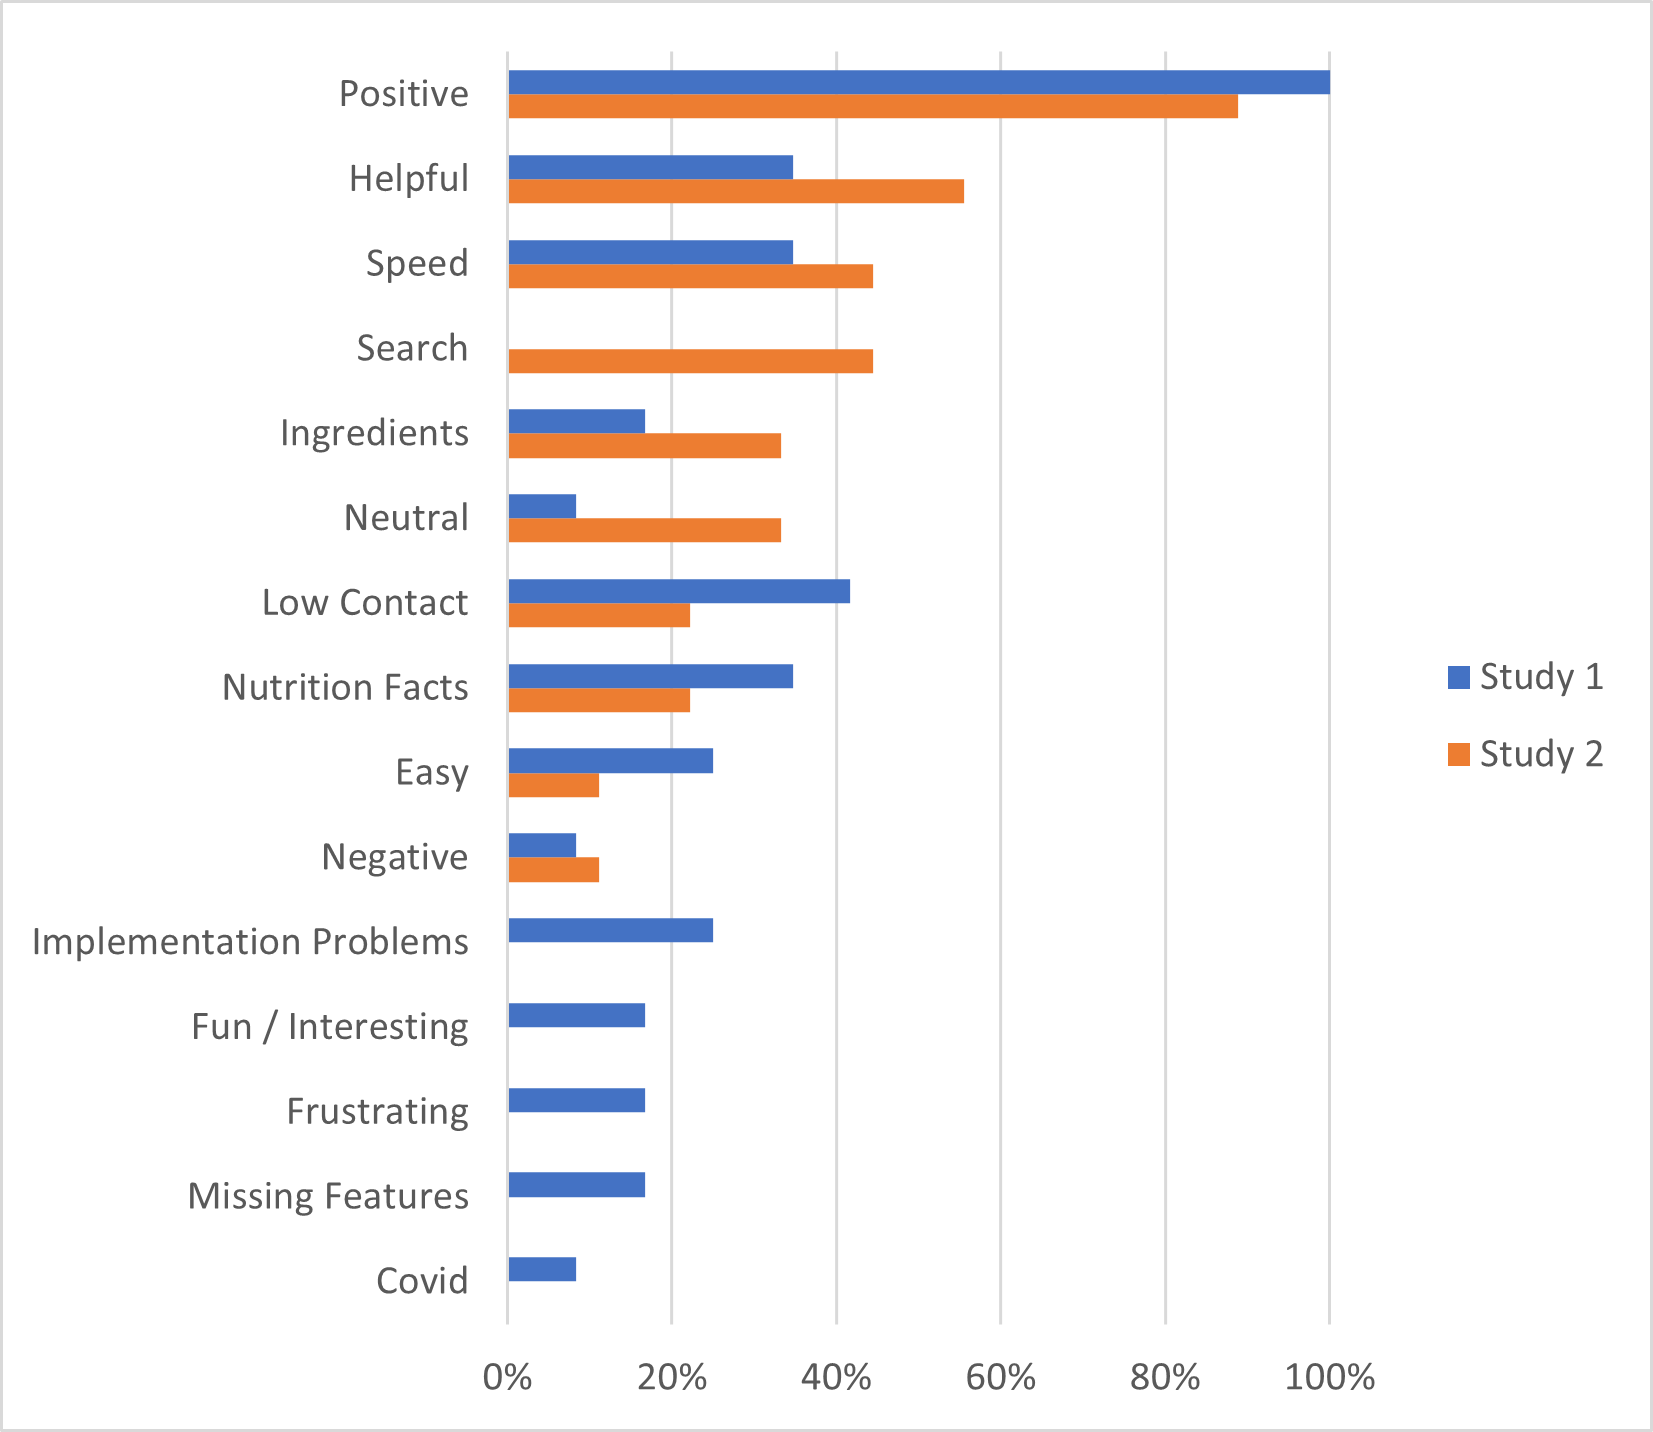
\includegraphics[width=\textwidth]{Images/experience themes study 2.png}
        \caption{Themes sorted by Study 2 percentages}
        \label{fig:exp-themes-study2}
    \end{subfigure}
    \caption{Studies 1 \& 2: Shopping experience comment theme frequency.}
    \label{fig:experience-themes}
\end{figure}

\newpage
\begin{enumerate}
    \item[] \textbf{Question: } Were you able to identify relevant allergens? Was the item information menu augmentation readable?
    \item[] \textbf{Response Analysis: } 100\% of participants answered "Yes" to the question on identifying allergens. Menu rotation and occlusion by other elements were major issues in the original prototype, reflected in Figure \ref{fig:readability1}. These issues were addressed in version 2.
\end{enumerate}


\begin{figure}[h]
    \centering
    \begin{subfigure}[]{.45\textwidth}
        \centering
        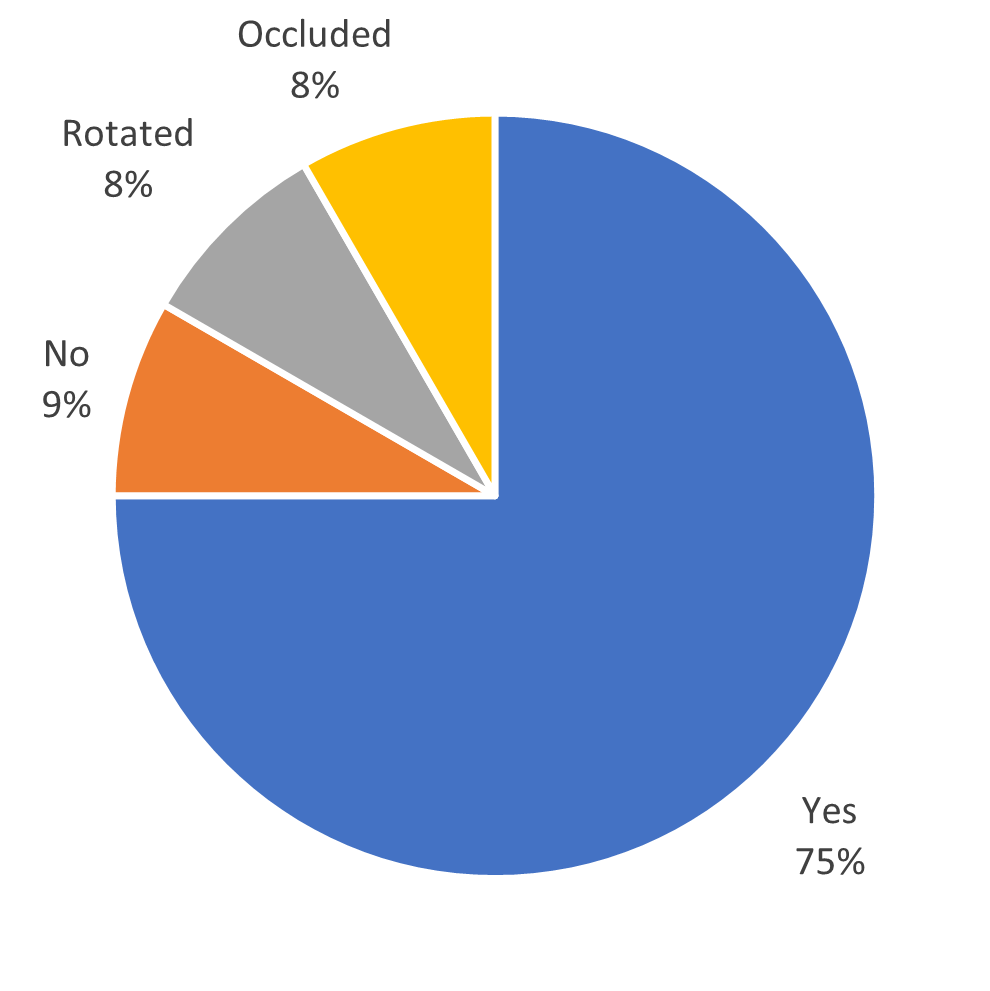
\includegraphics[width=\textwidth]{Images/readability study 1.png}
        \caption{First Study}
        \label{fig:readability1}
    \end{subfigure}
    \begin{subfigure}[]{.45\textwidth}
        \centering
        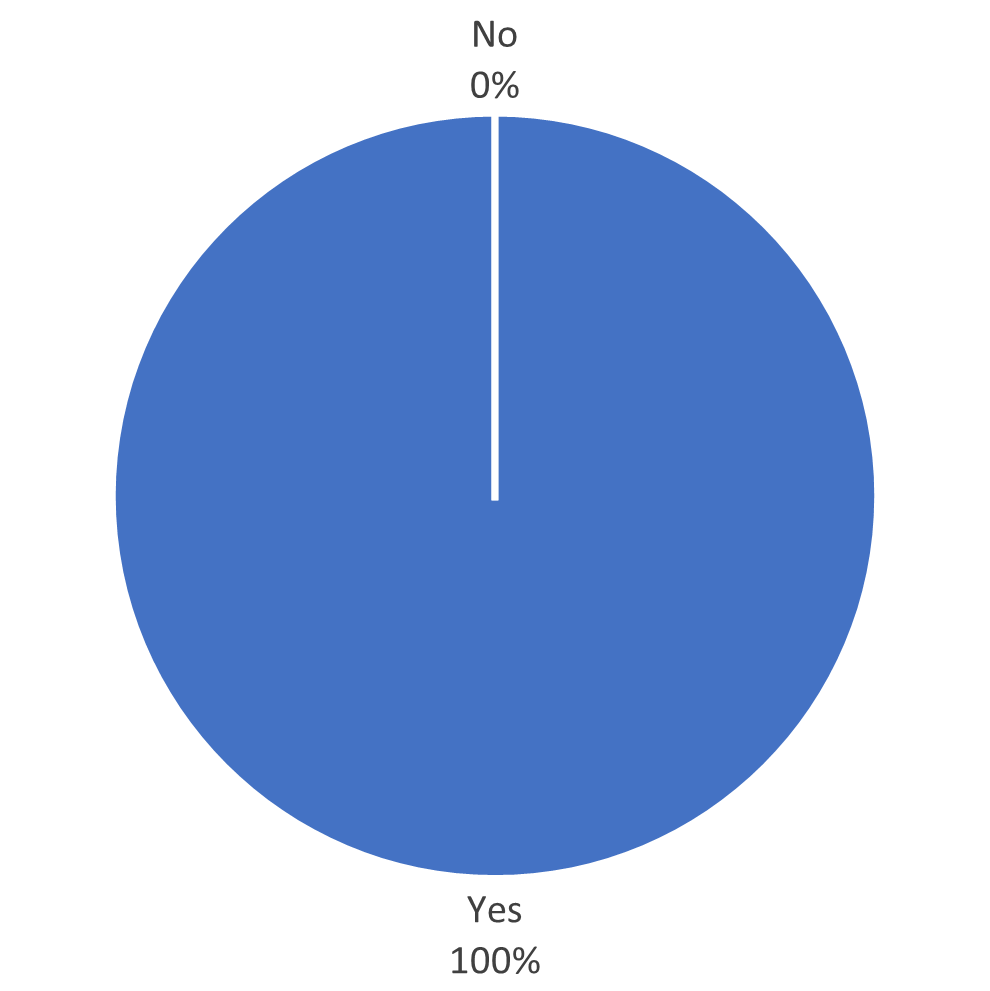
\includegraphics[width=\textwidth]{Images/readability study 2.png}
        \caption{Second Study}
        \label{fig:readability2}
    \end{subfigure}
    \caption{Studies 1 \& 2: Was the item information menu augmentation readable?}
    \label{fig:readability}
\end{figure}

\begin{enumerate}
    \item[] \textbf{Question: } Does not having to install an app improve the likelihood of using the system?
    \item[] \textbf{Response Analysis: } The majority of participants in both studies responded "Yes" to this question (see Table \ref{fig:no-download}), with a noticeable increase in positive-type themes during Study 2. The themes in Figure \ref{fig:web app-theme} align well with what we observed during the trials. 
\end{enumerate}

\begin{figure}[h]
    \centering
    \begin{subfigure}[]{.45\textwidth}
        \centering
        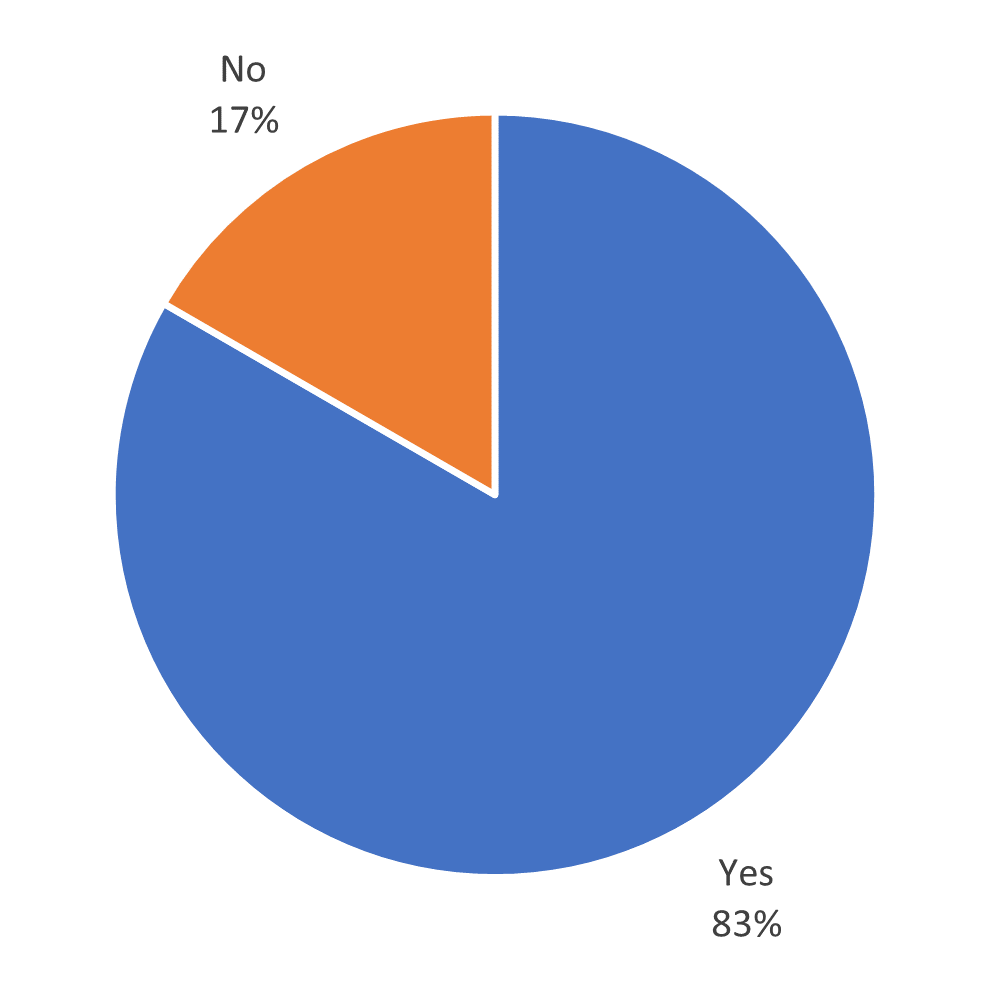
\includegraphics[width=\textwidth]{Images/web impact study 1.png}
        \caption{First Study}
    \end{subfigure}
    \begin{subfigure}[]{.45\textwidth}
        \centering
        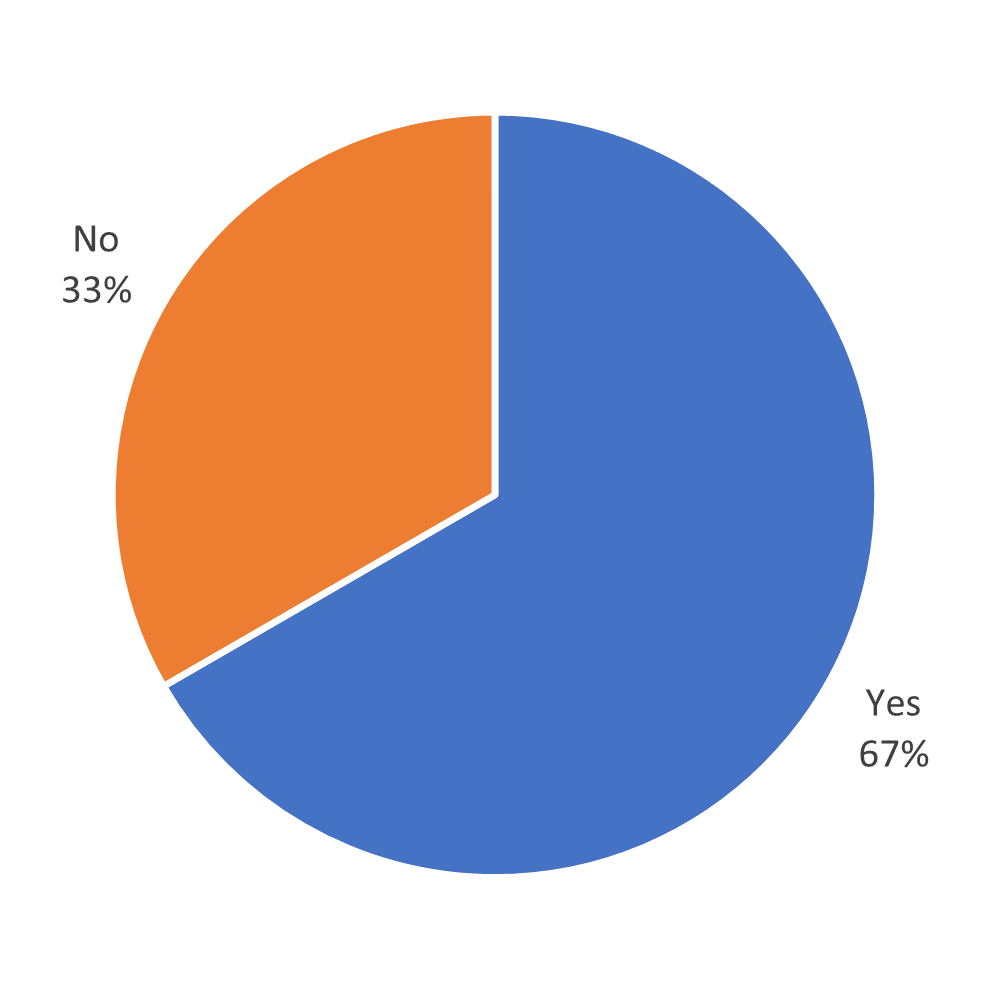
\includegraphics[width=\textwidth]{Images/web impact study 2.png}
        \caption{Second Study}
    \end{subfigure}
    \caption{Studies 1 \& 2: Was not having to install an app a positive of our system?}
    \label{fig:no-download}
\end{figure}

\begin{figure}[h]
    \centering
    \begin{subfigure}[]{.45\textwidth}
        \centering
        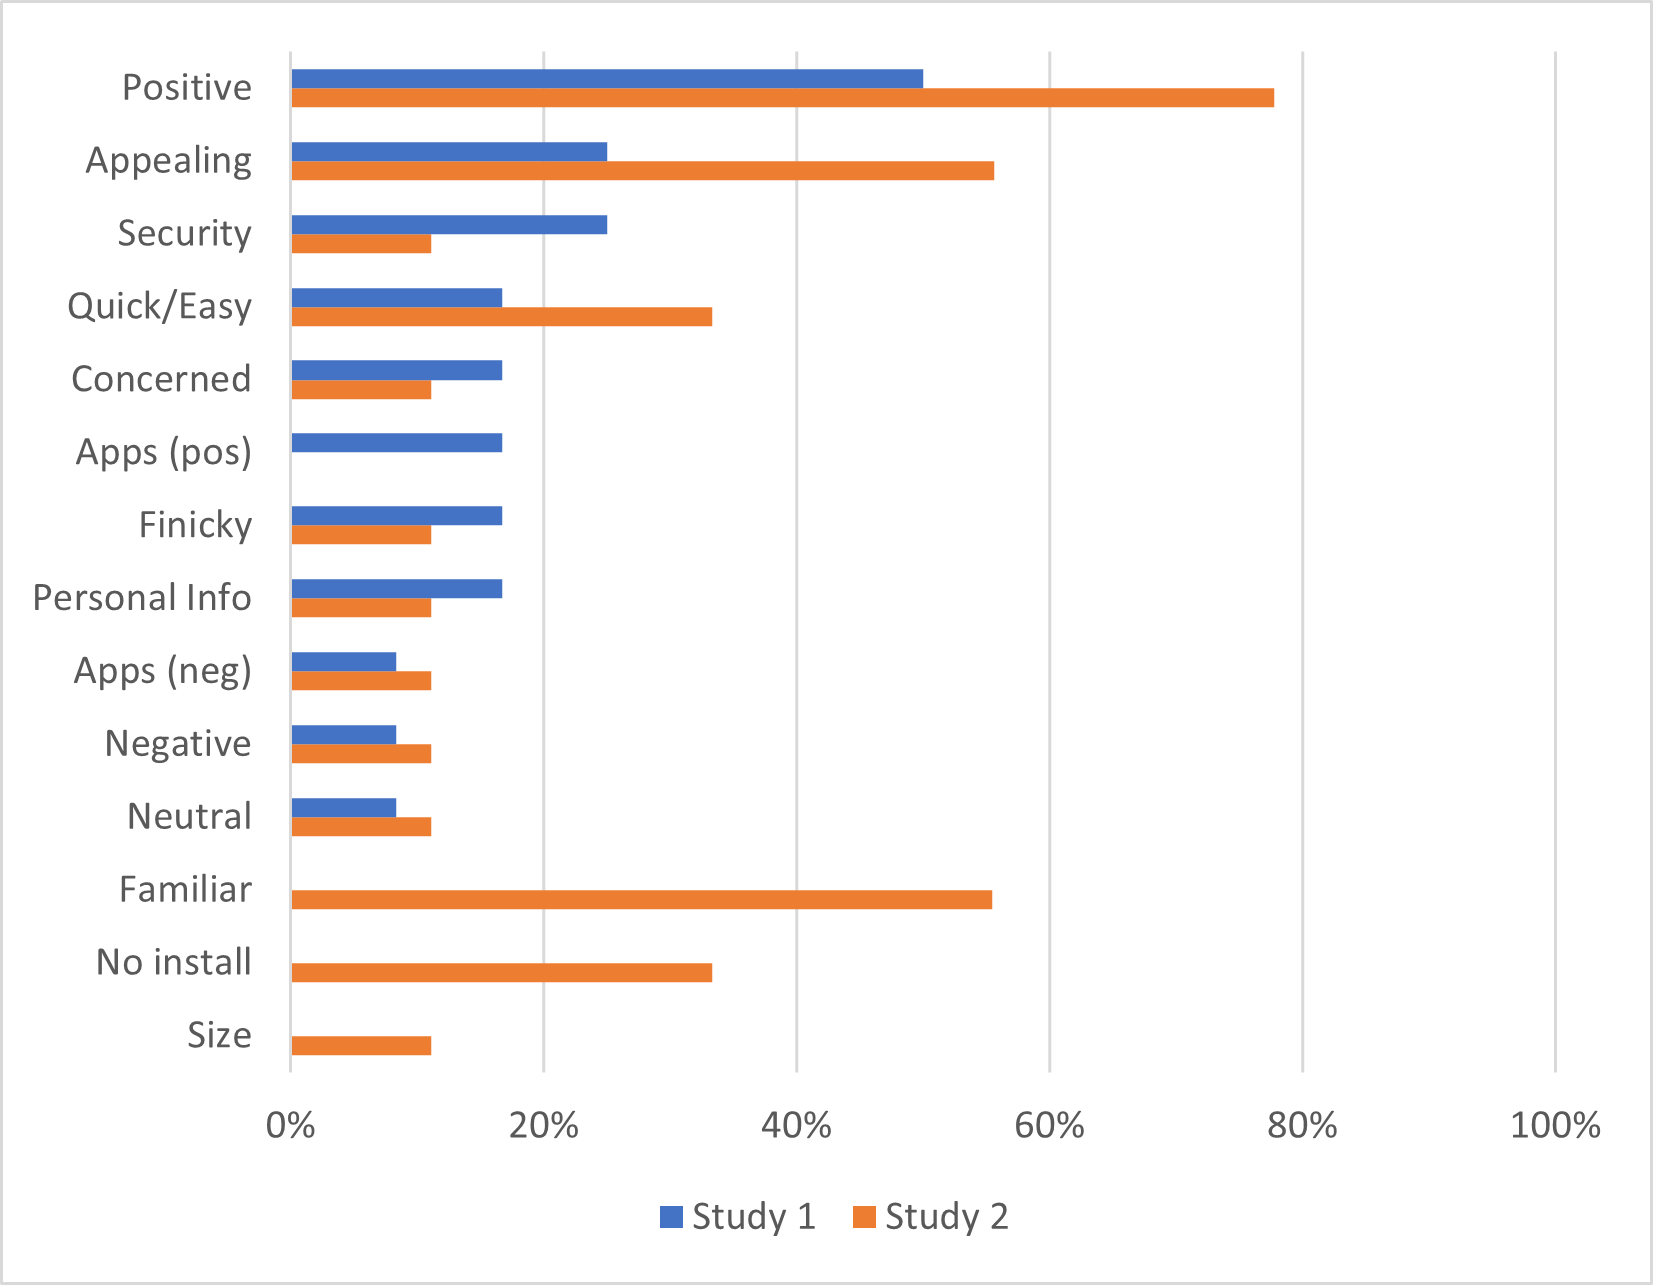
\includegraphics[width=\textwidth]{Images/web app themes study 1.png}
        \caption{Themes sorted by Study 1 percentages}
        \label{fig:webapp1}
    \end{subfigure}
    \begin{subfigure}[]{.45\textwidth}
        \centering
        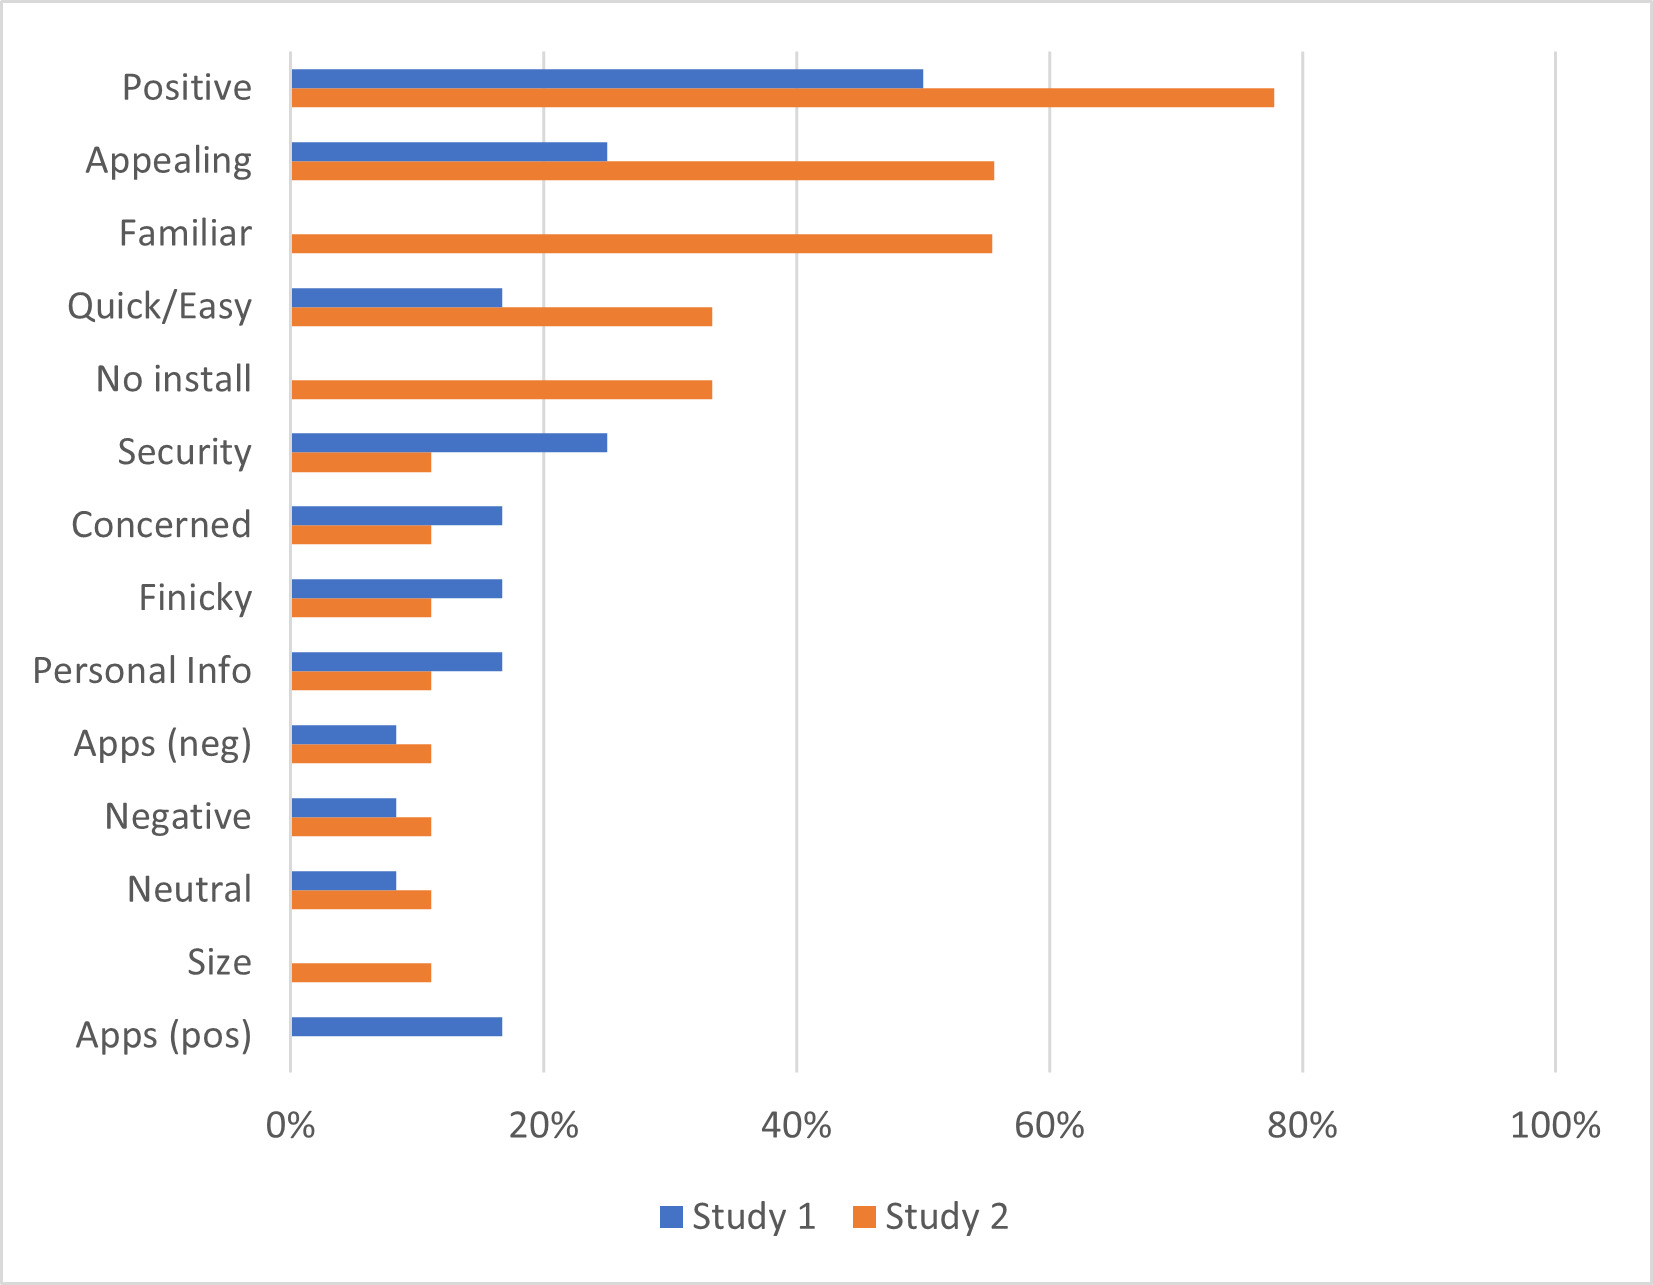
\includegraphics[width=\textwidth]{Images/web app themes study 2.png}
        \caption{Themes sorted by Study 2 percentages}
        \label{fig:webapp2}
    \end{subfigure}
    \caption{Studies 1 \& 2: Web-app impression theme frequency.}
    \label{fig:web app-theme}
\end{figure}
\pagebreak
\begin{enumerate}
    \item[] \textbf{Question: } Are there any features you would like to see added?
    \item[] \textbf{Response Analysis: } We asked participants what features they would like to see added after both tests. Answers from the first study were used to improve the system before the second user study. Table \ref{tab:missing-features} lists the suggested features, whether they were already functional requirements, and their implementation status. 
\end{enumerate}

\begin{table}[h!]\centering
\caption{Studies 1 \& 2: Features participants wanted to see added}\label{tab:missing-features}
\ra{1.2}
    \resizebox{\textwidth}{!}{%
        \begin{tabular}{@{}llll@{}}
        \toprule
            \textbf{Study \#}   &   \textbf{Feature}    &   \textbf{Functional Req.}    &   \textbf{Status} \\
        \midrule
            1      & Non \acrshort{ar} info menu      & No  & Outside scope         \\
            1      & Personalized info                & Yes & Implemented           \\
            1      & Reduce clutter when menu open    & No  & Implemented           \\
            1      & Add to list function             & No  & Outside scope         \\
            1      & Better UI for entering \acrshort{ar}        & No  & Partially implemented \\
            1      & More informative marker augments & Yes & Implemented           \\
            1      & More detailed information        & No  & Outside scope         \\
            1      & Search for ingredients and nutrition values & Yes & Implemented     \\
            2      & Customizable symbols             & No  & Outside scope         \\
            2      & Scroll bar for ingredients       & Yes & Future work           \\
            2      & Review section                   & Yes & Future work           \\
            1 \& 2 & Compare items                    & Yes & Future Work           \\
        \bottomrule
        \end{tabular}%
    }
\end{table}

\pagebreak
\begin{enumerate}
    \item[] \textbf{Question: } Would you continue to use an app like this in the future?
    \item[] \textbf{Response Analysis: } The majority of participants in both studies responded "Yes" to this question (see Table \ref{fig:no-download}, with a noticeable increase in positive-type themes during Study 2. The themes highlighted in Figure \ref{fig:web app-theme} align well with what we observed during the trials. 
\end{enumerate}

\begin{figure}[h]
    \centering
    \begin{subfigure}[]{.45\textwidth}
        \centering
        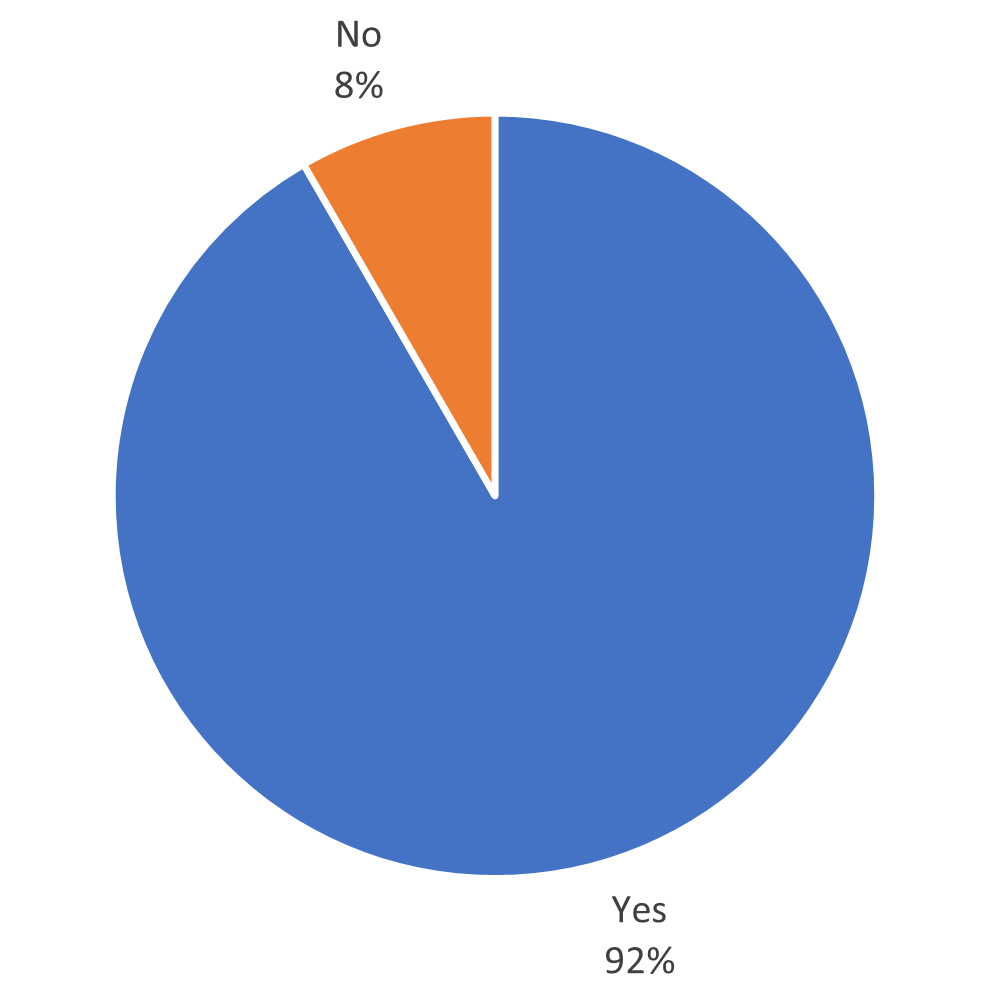
\includegraphics[width=\textwidth]{Images/future use study 1.png}
        \caption{First Study}
        \label{fig:future1}
    \end{subfigure}
    \begin{subfigure}[]{.45\textwidth}
        \centering
        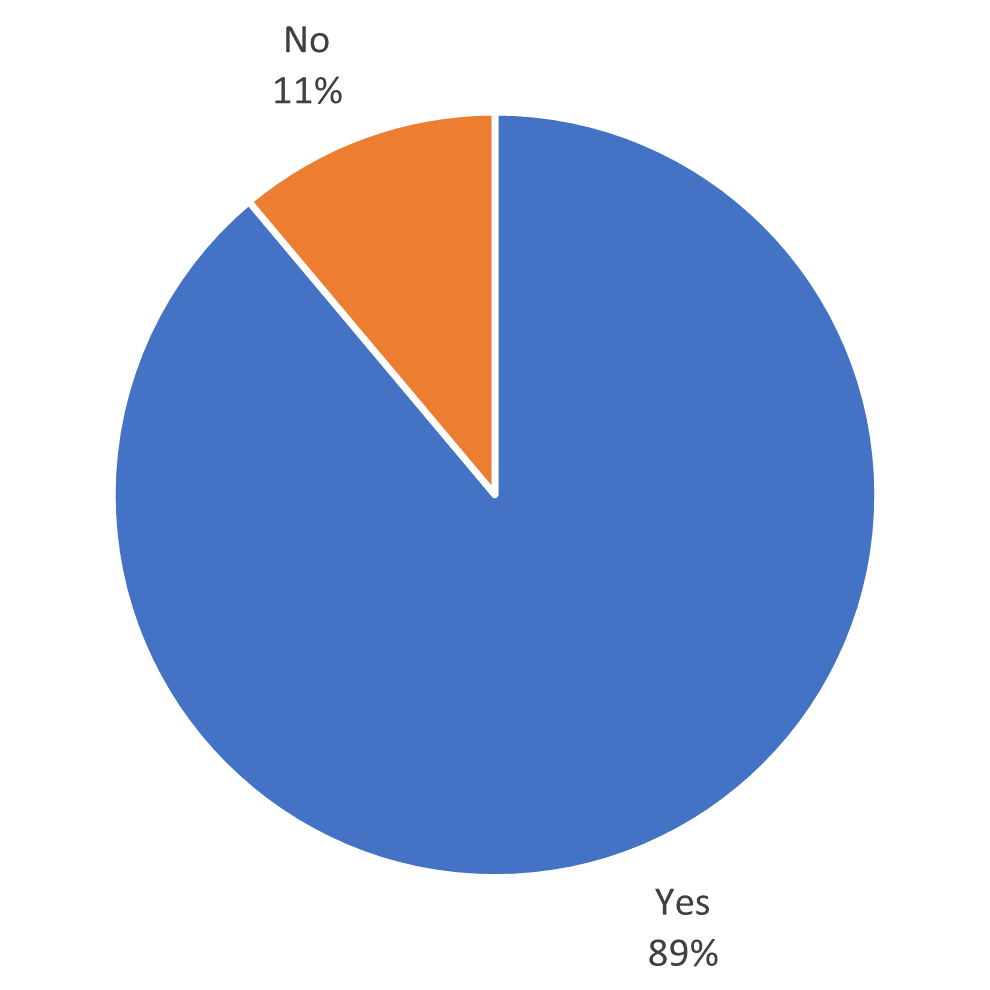
\includegraphics[width=\textwidth]{Images/future use study 2.png}
        \caption{Second Study}
        \label{fig:future2}
    \end{subfigure}
    \caption{Studies 1 \& 2: Would users want to use this again in the future?}
    \label{fig:future-use}
\end{figure}

\pagebreak
\section{Chrome Lighthouse Benchmark}
Google Chrome provides a mobile and desktop webapp performance assessment tool. We ran the benchmarks on the final app version used in Study 2. Figure \ref{fig:light-scores} shows the scores for the four categories Lighthouse assesses. Figure \ref{fig:light-perf} breaks down the scoring criteria for performance, our worst score. 
\begin{figure}[h]
    \centering
    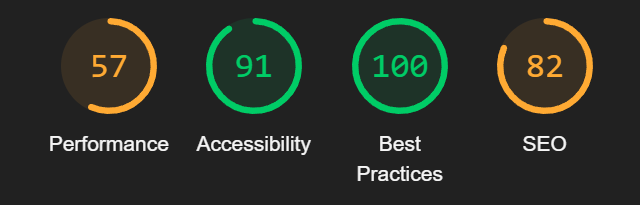
\includegraphics[width=0.7\linewidth]{Images/lighthouse scores.png}
    \caption{Overall Lighthouse scores}
    \label{fig:light-scores}
\end{figure}

\begin{figure}[h]
    \centering
    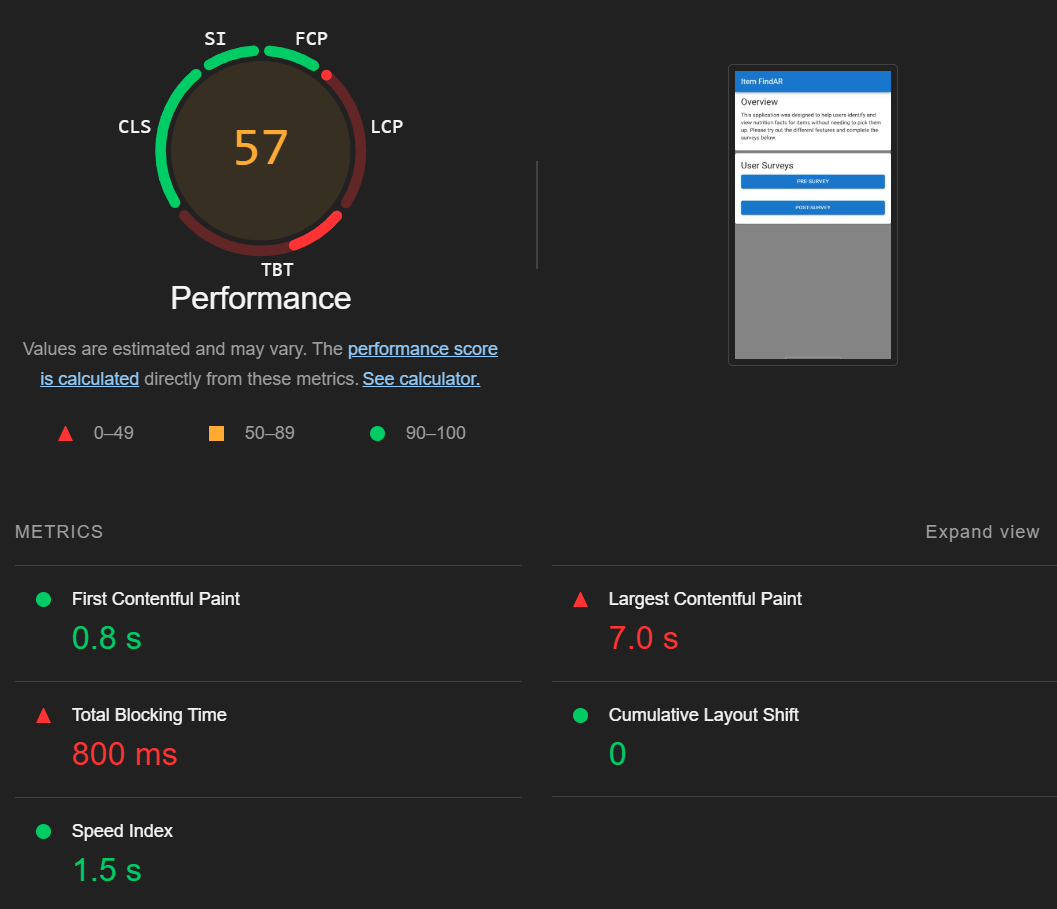
\includegraphics[width=0.7\linewidth]{Images/lighthouse performance.png}
    \caption{Lighthouse performance benchmark}
    \label{fig:light-perf}
\end{figure}

\chapter{ANALYSIS AND CONCLUSIONS}
In this chapter we reflect back on our research questions and goals and discuss how the data generated from the surveys and participant comments during the testing supports those goals. We also comment on how different issues and challenges during development affected the trials and user experience.

\section{Research Question Analysis}
\subsection{Can items be recognized without third-party identifiers?}
Yes, and with high speed and accuracy. The YOLOv8-XL model proved to be excellent, providing snappy results in a broader range of circumstances than initially expected. The lab-set model proved to be effective in a range of locations similar to the original training location (the lab space, white desk, plain background with desks and other objects), regardless of lighting conditions. We were able to run tests in various locations including upstairs in the IST commons, and in the IST classrooms. All the spaces shared white desks and walls with grey floors, similar in appearance but varying in lighting and surroundings. This bodes well for future work on expanding the locational usability.

We were able to recognize a range of objects from a range of angles, and often with partial occlusion, in a variety of lighting situations. Unfortunately, our WebXR surface detection implementation was painfully slow and the only visual feedback method for users. Nearly every participant commented on how slow and inaccurate the detection was, despite the actual object detection taking a fraction of a second. Improvements to the alignment system in version 2 increased the marker placement noticeably during testing, and the accuracy improvement led to reduced user frustration, as evidenced by responses from users that participated in both studies. We currently suspect incompatibility issues with the rendering engine to be the cause of the lag. Providing some sort of visual feedback that detection occurred, even before markers are placed, is our current proposed solution, covered further in Chapter 7.

\subsection{What steps are needed to ensure user data is protected?}
There are two main aspects to this question, the emotional one on the part of the user, and the practical one: 
\begin{enumerate}
    \item What is required to reassure the user their data is secure?
    \item What is required to deploy WebXR applications to production?
\end{enumerate}
Our solution to the first question was to collect as little data as possible, and to allow the user to retain full control over their data at all times. No account was required, and user preference storage was implemented through an opt-in cookie that could be disabled at any time. The only data stored in the cookie was the relevant allergen and dietary restriction settings, no identifying data was collected. 

Addressing the second question, a properly implemented technical solution has little impact on the end user's experience beyond "this site is secure" messages and the "https" address header. Letting any of the necessary \acrshort{ssl} certificates expire or making mistakes in configuring the application parts (database, client, backend, nginx, etc.) results in multiple safety warnings and failures to connect. 
We achieved the basic levels of security and encryption necessary to ensure a positive user experience as detailed in Chapter 3, with two major security flaws present in the final version. 
One was the Cypher DB queries dynamically generated on the client. We implemented write protection on the database and no user credentials or data existed in the database, but a skilled user could edit the queries in the browser console to return the entire database. This could be a major vulnerability and needs addressing in the future. 
The second security flaw is a general issue with the design of the computer vision backend server and was outside the scope of this project. We discuss possible solutions in Chapter 7.

\subsection{How can we maximize the comfort of users to encourage them to use our system?}
We failed in our goal of unified multi-platform development through the use of web APIs, but users still expressed appreciation of the benefits of the PWA deployment model. The general sentiment was that the web app, especially when installed on the home screen as a PWA, was nearly indistinguishable from a normal app without the need for a full download. Table \ref{tab:sec-responses} contains some relevant quotes from the post-test surveys from participants about the web and security aspects of the application. 

\begin{table}[h]\centering
\caption{Studies 1 \& 2: Participant quotes on webapp benefits and security of our system.}\label{tab:sec-responses}
\ra{1.2}
    %\resizebox{\textwidth}{!}{%
        \begin{tabular}{@{}l >{\raggedright\arraybackslash}p{\dimexpr 0.6\linewidth-2\tabcolsep} @{}}
            \toprule
                \textbf{Topic}  &   \textbf{Quotes} \\
            \midrule
                    Web vs Native Apps & "I like the idea of not having the app on my phone."                      \\ 
                    & "not having to download it is nice, but otherwise functions very similar" \\ 
                    & "It seems more convenient for people with less storage space..."          \\ 
                    & "Close enough that I wouldn't know if it wasn't revealed" \\
                    \\
                    Security & "I think that for security reasons, this is a good idea"                  \\  
                    & "Popular and data collection minimizing"                                  \\  
                    &  "quick and easy; do not have to provide personal information; do not have to load up my phone with yet another app \\
            \bottomrule
        \end{tabular}%
    %}
\end{table}

Analysis of the NASA TLX results from both studies clearly indicate the primary workload factor was Effort. In the first study, the Physical Demand and Frustration were positively correlated, and Physical Demand and Effort were strongly positively correlated. From participant comments during and after the trials, and direct observation during personal testing, having to move the phone around to get a surface detection, only for it to be incorrect or inaccurate, was deeply frustrating. In version 2 we improved the accuracy and placement significantly, and reduced the amount of movement required, but the WebXR issues persisted. This directly impacted user perception of the computer vision detection for the first question, as the marker system was the only feedback visible to the end user. These WebXR detection issues are not present in samples provided by the immersive-web group, indicating issues with our implementation.

Maintaining consistent performance was a major aspect for user enjoyment, especially with the client/server model for the image processing. We cover this more in the next section and Chapter 7.

\subsection{What is needed to ensure consistent performance across devices?}
We chose to limit the number of frames sent to the detection server and to crop them in advance to reduce latency issues and bandwidth usage. Sending the image data directly over websockets to our local PC through a forward proxy (Ngrok) was significantly faster than re-encoding the image and sending the data to a REST API; these results were strongly network speed dependent. The lab testing room is located in an inner room in the university's research building, with thick concrete walls. We found that connecting to the building's WiFi was required for performance better than one frame received every couple seconds at best. 

Some form of dedicated graphics processor is required to run the model efficiently. When we were investigating AWS Sagemaker for our deployment method, we realized even the expensive instances with 20 or more CPUs were far too slow compared to our local development machine with a Nvidia 3080, and that AWS would not approve our use of a GPU instance without significant time investment to prove our authenticity and need. 
\begin{table}[h]\centering
\caption{Average model frame processing speeds}
\label{tab:frame-proc}
\ra{1.2}
    \begin{tabular}{@{}lcr@{}}
        \toprule
            \textbf{Graphics Card (GPU)}    &   \textbf{Memory}   &   \textbf{Average Frame Processing Time}  \\
        \midrule
            Nvidia RTX 3080 (Laptop)     & 16 GB VRAM   & 20-30 ms     \\
            Nvidia RTX 3050ti (Laptop)   &  4 GB VRAM   & 40-70 ms     \\
            Nvidia GTX 1080 (Laptop)     & 8 GB VRAM    & 30-50 ms     \\
            Intel Core i7-8750H CPU      & 16GB RAM     & 2500-2700 ms \\
            Intel Core i7-12700H CPU     & 16 GB RAM    & 1400-1500 ms \\
        \bottomrule
    \end{tabular}%
\end{table}
Table \ref{tab:frame-proc} contains average recognition times per frame by the \acrshort{yolo} model on the three test PCs we used to run the backend. Better hardware allows for real-time 30 frames-per-second processing.  Our system sent frames periodically (every second), lowering the requirements significantly.

\subsection{How familiar are potential users with other Augmented Reality applications?}
The participant statistics listed at the beginning of Chapter 5 indicate that the majority of participants had at least some experience with \acrshort{ar} apps in the past. Most users that responded to the short answer section responded positively, especially those that play Pokemon Go or have used the \acrshort{ar} apps for the Nintendo 3DS. The surveys referenced Google Maps as an \acrshort{ar} app and multiple participants mentioned this as a positive example, but this was unintentionally misleading. We needed to clarify that we meant the \acrshort{ar} walking directions tool specifically, which few participants had actually used or were aware of. We adjusted for this in some of our results; the full responses can be found in Appendix B.

\section{Main Research Question}
\begin{itemize}
    \item[] \textbf{Question: } \textit{Can the grocery shopping experience be improved via the use of Mobile Augmented Reality, specifically finding and identifying the contents of products?}
    \item[] \textbf{Analysis: } The results are clear: there is high demand for a mobile tool for scanning and searching for items in shopping or other situations. The theme analysis of participant responses in Chapter 5 indicates that user responses to and opinions of the system concept and prototypes was overwhelmingly positive. During the trials, participants were excited to try the app and were very patient with the frequent disruptive errors and issues. Table \ref{tab:use-quotes} contains some samples of direct quotes from participants on their opinions of the concept and whether they found the system helpful. 

\end{itemize}

\begin{table}[h]\centering
\caption{Participant quotes on whether the app was useful.}
\label{tab:use-quotes}
\ra{1.2}
    \begin{tabular}{@{}l >{\raggedright\arraybackslash}p{\dimexpr 0.6\linewidth-2\tabcolsep} @{}}
        \toprule
            \textbf{Topic} & \textbf{Quote} \\
        \midrule
            Value to User & "...a lot easier to find out nutritional info than normal" \\  
            & "Saves time in identifying what I want to avoid"           \\  
            & "I'm usually very handsy so this way I can feel better about not touching product I probably won't buy." \\ 
            & "Made finding the products I was looking for easier..."    \\  
            & "Easy to learn nutritional information without handling the products..." \\
        \bottomrule
    \end{tabular}%
\end{table}

\section{Final Conclusions}
This research sought to assess how accepting possible users are of a mobile augmented reality shopping tool for finding and getting info on items in stores, and to identify key methods and design principles for the implementations of such a system. We first identified what elements and design factors should be preserved from the previous research with the HoloLens. We created a list of functional requirements for our system based on this and a review of past literature related to \acrshort{ar} shopping tools. Once the requirements were settled and all the necessary programming \acrshortpl{api} and libraries were identified, we then implemented a proof of concept, gathered feedback on usability, made improvements to the system, and repeated the user study. Participants across both studies expressed enthusiasm and excitement during the tests and in the written responses to the surveys after. Most participants also responded that they would like to use a polished version if one were available. We consider this to be clear evidence supporting our hypothesis that such a tool would be useful and desirable.

Analysis of the workload index scores identified clear positive correlations between factors: Frustration and Physical Demand for the first study, and Effort and Physical Demand for the second. Effort was also the highest scoring workload factor in both studies. This indicates that the greatest negative impact on users was the effort required to get a successful result, and that the physical demands of moving the phone around to successfully place the virtual markers contributed significantly to user frustration and effort. The overall workload score for the second study was higher than the first, implying the second version was more difficult to use. This aligns well with the change in scores between both studies for the SUS, which dropped slightly. Generally, this would indicate that the system was worse for users in the second trial; participant comments during and after the trials instead suggest the increase in features and stability led to users assessing the system itself with greater scrutiny, rather than focusing on the general concept.

Overall, our system achieved the goal of producing a system that could identify items without markers, locate them in the user's space, and provide robust nutritional information, all from the user's mobile web browser. We developed a functional proof of concept for the methods required to make such a system possible and have included all the necessary and useful materials required to continue research on this topic. Participant responses from both studies strongly indicate that potential users care about what's in their food, have difficulty identifying that information from reading the package, and would greatly appreciate a digital tool to improve the process. 
Users also commented that the lack of app downloads and user account requirements was a major positive for the system, as was reducing contact with food items before purchase. The only downsides participants mentioned consistently were the technical implementation issues, commenting during the trials and in the surveys that the \acrshort{ar} concept was fun to use but the accuracy and movement issues detracted from the experience. We discuss areas for improvement and future research in the next chapter.

\chapter{FUTURE WORK}
There are several opportunities for further research and improvement of this system. We list some of them here and propose possible methods for addressing them. The most important areas are improving surface detection speed for WebXR and improving frame transmission to the backend server.

\section{WebXR Hit Testing Speed and Accuracy}
This is a valuable area for research, as there is little documentation on developing \acrshort{ar} visualizations for computer vision data on the web. We based our system off a sample for native android written in Kotlin, and the Immersive Web group's \verb|raw-camera-access| documentation. When we encountered incompatibilities with the Three.js engine, there were few examples to be found, and few people that could help. Producing a fully documented tutorial for aligning WebXR anchor points with computer vision data would be a great asset for future research.
Our issues with the long delay before WebXR makes a successful hit-test (detects a surface) and more recent issues with the \verb|raw-camera-access| API causing a long delay every frame are not present when we test the Immersive Web samples. We have not verified the issue, but the likely cause is either programmer error, or worsening incompatibility issue with Three JS. 

\section{Client/Server Data Transmission}
HTTP transmission through a REST API is the standard method for most computer vision APIs. Our goal was to maximize the transfer speed from the client to the server, opting for websockets to avoid the encoding delay for images with HTTP. We did not run proper timing benchmarks to measure how long the delay was, nor did we try any optimizations for the frame beyond cropping it to reduce size. For the marker system we developed, this was adequate, but a faster option would be necessary for the segmentation mask selection UI we originally intended to use for the search function. Possible options include downscaling or compressing the frames, researching how live streaming in high resolution works, and benchmarking the performance of YOLO's lighter weight models on the mobile hardware directly. Eliminating the need for the server in some cases (a smaller model for common items) could allow for proper offline functionality.

\section{UI/UX Usability Improvements}
We planned this thesis and user study(s) to focus on testing different UI designs in an \acrshort{ar} setting. Developing and improving the base system took precedence over UI variations, and the scope shifted. Now that there's a basic example of what needs to be implemented to run a markerless \acrshort{ar} experience on the mobile web, progress can be made to improve the user experience. Much of the workload and UX issues stemmed from other issues listed in this section; we would continue our UI research in two areas:
\begin{enumerate}
    \item Determine the best option selection method that does not resize the window
    \item Rebuild the augmented nutritional menu in Three JS
\end{enumerate}
Our menu overlay system for selecting ingredients and other search criteria relied on auto-complete search boxes for categories with long lists. Google's default keyboard, Gboard, automatically appears and causes sometimes fatal errors (rapid white flashing that could trigger a seizure), as a change to the \acrshort{ar} scene's window size occurs. Some method for selecting options from a long list while utilizing the menu overlay needs to be devised. A related issue occurs when users inevitably want to try the app in landscape mode as only portrait is supported. 

The library we used for the augment menus had major performance issues, and little documentation for their React compatibility. Enabling users to either expand the ingredient panel or scroll to see more was one of the few requirements we were unable to implement. In future research, we would attempt to reimplement the menus with the HTML element embedding system provided by ThreeJS. This would eliminate extra dependencies and hopefully improve the reliability of the interface.

Lack of auto-focus control for WebXR is a great hindrance for this type of application. The setting can be enabled easily for native apps, but the Immersive Web working group only recently changed their position on allowing developers to enable the focus, and Google has not implemented a toggle for the setting into their Chromium browser as of yet. Without the auto-focus, applications requiring near vision through the device are rendered partially unusable by how blurry the camera view is. The only option currently seems to be requesting that the Chromium developers implement the feature.

The last important user interaction issue was the lag in visual feedback between the recognition of the item, and the rendering of the marker. Many participants complained or commented that they didn't think the recognition part worked well. Verifying the results with the logs revealed that correct coordinates and classes for the items were returned from the server; if the marker placement system speed cannot be increased, then another method of temporary feedback needs to be investigated. One option would be to place loading spinners on the screen to line up with where items are before the markers are placed.

\section{Vision Model Generality}
The ideal testing environment would be a small market or shop setting, similar to the Mosaic Cafe as we originally intended. Our Mosaic model dataset was produced manually until midway through the project, leading to an unbalanced number of annotated classes, as seen in Table \ref{fig:mosaic-dataset}. The Home and Lab datasets had around 300 instances of each class, and the resulting models performed well in a range of circumstances as long as the backgrounds were similar. In a final product use case, users may want to use the app in a wide range of settings. Research on how to provide accurate results in the widest number of locations for the same classes while minimizing the human effort required for data labelling would be our next step for research on the model.

\section{Scaling for Production}
Our system works well as a proof of concept; deploying as a real service would require solving two major problems: dataset creation and hardware for training and running the models. The ideal version would be a system users could scan items with in any location, whether a store or their friend's house. We used YOLO for our model, but a slower model that works in a broader range of backgrounds could easily replace it, as the system only requires coordinates and identifiers to place markers. 

The minimum hardware required for acceptable performance was some form of dedicated \acrshort{gpu}; when testing the Sagemaker deployment, the fastest image processing time we could get was around 1500 milliseconds using one of their more expensive \acrshort{cpu} instances. We consider this just barely acceptable, anything longer and users started to feel impatient. A full investigation of what type of hardware would be needed to support multiple users at scale is required before an estimate of cost can be made. One option would be to allow users to have the option to host the backend themselves. Running the server was very easy, especially with the forward proxy service. Cloud hosting is the traditional method, other monetization options besides selling data would need to be devised if the focus on user data security is to be preserved. Dataset production faces similar challenges of requiring significant manual labor and hardware.

%% Currently adding the references to the table of contents is not automatic
%% So we are forced to do it manually.

%% TODO: This is not a fix. This line has to come after the \chapter command
%% in order for the correct page to be inferred for the table of contents.
\renewcommand{\bibsection}{\topskip=1in\chapter*{REFERENCES}\topskip=0in \addcontentsline{toc}{chapter}{REFERENCES}}

%% Generates the bibliography.
\singlespacing
\bibliographystyle{IEEEtranbib}
\bibliography{citations}

\doublespacing
\begin{appendices}
\addtocontents{toc}{\setlength{\cftchapnumwidth}{1em}}
\renewcommand{\appendixname}{APPENDIX}
\addtocontents{toc}{\setcounter{tocdepth}{0}}
\addtocontents{toc}{\protect\renewcommand{\protect\cftchappresnum}{}}

\chapter{Code Samples}
\section{External Links}
\begin{table}[h]\centering
\caption{Links to code repositories and datasets}\label{tab:repos}
\ra{1.3}
    \begin{tabular}{@{}l p{\dimexpr 0.5\linewidth-2\tabcolsep} >{\raggedright\arraybackslash}p{\dimexpr 0.3\linewidth-2\tabcolsep}@{}}
        \toprule
            \textbf{Type}   &   \textbf{Link}   &   \textbf{Description}    \\
        \midrule
            Google Sheet    &   \url{https://docs.google.com/spreadsheets/d/1M7oUOY7P\_yl4z5Z4pFSgaGZCc02WE4VKXe6nSkH\_1LI/edit?usp=sharing}    &   Mosaic Cafe datasheet   \\
            Github          &   \url{https://github.com/croche2574/Item-FindAR} &   Web Client repo \\
            Github          &   \url{https://github.com/croche2574/Yolo-API}    &   Backend Server repo  \\ 
            Github          &   \url{https://github.com/croche2574/Label-Studio-YOLOv8-backend} & Label Studio active learning script   \\
            HuggingFace     &   \url{https://huggingface.co/collections/colterroche/item-findar-66cdfa3e5ad37bd8fb32d2b4}   &   Datasets \& Models  \\
        \bottomrule
    \end{tabular}%
\end{table}

\filbreak
\section{Neo4j Import Script}
\singlespacing
\begin{lstlisting}[language=Cypher]
//Load Data

//Clear Previous Data
MATCH (i:Ingredient) DETACH DELETE i;
MATCH (i:Item) DETACH DELETE i;
MATCH (n:Nutrient) DETACH DELETE n;
MATCH (a:Allergen) DETACH DELETE a;
MATCH (t:ItemTag) DETACH DELETE t;

//Uncomment after first run 
//DROP INDEX itemNames;

//Create Nutrient Nodes
CREATE (:Nutrient {name:'Calories'});
CREATE (:Nutrient {name:'Total Fat', unit: 'g'});
CREATE (:Nutrient {name:'Saturated Fat', unit: 'g'});
CREATE (:Nutrient {name:'Cholesterol', unit: 'mg'});
CREATE (:Nutrient {name:'Sodium', unit: 'mg'});
CREATE (:Nutrient {name:'Total Carbohydrate', unit: 'g'});
CREATE (:Nutrient {name:'Dietary Fiber', unit: 'g'});
CREATE (:Nutrient {name:'Total Sugars', unit: 'g'});
CREATE (:Nutrient {name:'Added Sugars', unit: 'g'});
CREATE (:Nutrient {name:'Protein', unit: 'g'});
CREATE (:Nutrient {name:'Vitamin D', unit: 'mcg'});
CREATE (:Nutrient {name:'Calcium', unit: 'mg'});
CREATE (:Nutrient {name:'Iron', unit: 'mg'});
CREATE (:Nutrient {name:'Potassium', unit: 'mg'});
CREATE (:Ingredient:Additive {name: 'Caffeine', unit: 'mg'});

//Create Search Indexes
CREATE FULLTEXT INDEX itemNames FOR (i:Item|Ingredient) ON EACH [i.name];

//Load Ingredients
LOAD CSV WITH HEADERS FROM 'https://docs.google.com/spreadsheets/d/1M7oUOY7P_yl4z5Z4pFSgaGZCc02WE4VKXe6nSkH_1LI/pub?gid=184817080&single=true&output=csv' AS row

//Create Ingredient Nodes
MERGE (ing1:Ingredient {name: row.Ingredient})

//Attach Sub-Ingredients
WITH ing1, row
UNWIND split(row.Sub_ingredients, ';') as ingredient
MERGE (subIng:Ingredient {name:ingredient})
MERGE (ing1)-[r:CONTAINS_SUBINGREDIENT]->(subIng);

//Load Items
LOAD CSV WITH HEADERS FROM 'https://docs.google.com/spreadsheets/d/1M7oUOY7P_yl4z5Z4pFSgaGZCc02WE4VKXe6nSkH_1LI/pub?gid=531798652&single=true&output=csv' AS row

//Create Item Nodes
MERGE (item:Item {
    name: row.Item_name, 
    class_code: row.Class_code, 
    brand: row.Brand, 
    servings: row.Servings, 
    ingredient_list: row.Ingredients})

//Create and Attach Item Tags
WITH item, row
UNWIND split(row.Item_tags, ';') AS item_tag
MERGE (tag:ItemTag {name: item_tag})
MERGE (item)-[:TAGGED_AS]->(tag)

//Create Relations to Nutrition Data
WITH item, row
MATCH (n:Nutrient {name:'Calories'})
MERGE (item)-[r:CONTAINS_NUTRIENT]->(n)
SET r.amount = toInteger(row.Calories)

WITH item, row
MATCH (n:Nutrient {name:'Total Fat'})
MERGE (item)-[r:CONTAINS_NUTRIENT]->(n)
SET r.amount = toFloat(row.Total_fat_amt)
SET r.percentage = toFloat(row.Total_fat_per)

WITH item, row
MATCH (n:Nutrient {name:'Saturated Fat'})
MERGE (item)-[r:CONTAINS_NUTRIENT]->(n)
SET r.amount = toFloat(row.Sat_fat_amt)
SET r.percentage = toFloat(row.Sat_fat_per)

WITH item, row
MATCH (n:Nutrient {name:'Cholesterol'})
MERGE (item)-[r:CONTAINS_NUTRIENT]->(n)
SET r.amount = toInteger(row.Cholesterol_amt)
SET r.percentage = toFloat(row.Cholesterol_per)

WITH item, row
MATCH (n:Nutrient {name:'Sodium'})
MERGE (item)-[r:CONTAINS_NUTRIENT]->(n)
SET r.amount = toInteger(row.Sodium_amt)
SET r.percentage = toFloat(row.Sodium_per)

WITH item, row
MATCH (n:Nutrient {name:'Total Carbohydrate'})
MERGE (item)-[r:CONTAINS_NUTRIENT]->(n)
SET r.amount = toInteger(row.Carbs_amt)
SET r.percentage = toFloat(row.Carbs_per)

WITH item, row
MATCH (n:Nutrient {name:'Dietary Fiber'})
MERGE (item)-[r:CONTAINS_NUTRIENT]->(n)
SET r.amount = toInteger(row.Fiber_amt)
SET r.percentage = toFloat(row.Fiber_per)

WITH item, row
MATCH (n:Nutrient {name:'Total Sugars'})
MERGE (item)-[r:CONTAINS_NUTRIENT]->(n)
SET r.amount = toInteger(row.Total_sugar)

WITH item, row
MATCH (n:Nutrient {name:'Added Sugars'})
MERGE (item)-[r:CONTAINS_NUTRIENT]->(n)
SET r.amount = toInteger(row.Added_sugar)
SET r.percentage = toFloat(row.Sugar_per)

WITH item, row
MATCH (n:Nutrient {name:'Protein'})
MERGE (item)-[r:CONTAINS_NUTRIENT]->(n)
SET r.amount = toInteger(row.Protein)

WITH item, row
MATCH (n:Nutrient {name:'Vitamin D'})
MERGE (item)-[r:CONTAINS_NUTRIENT]->(n)
SET r.amount = coalesce(toInteger(row.VitD_amt), '-')
SET r.percent = coalesce(toFloat(row.VitD_per), '-')

WITH item, row
MATCH (n:Nutrient {name:'Calcium'})
MERGE (item)-[r:CONTAINS_NUTRIENT]->(n)
SET r.amount = coalesce(toInteger(row.Cal_amt), '-')
SET r.percent = coalesce(toFloat(row.Cal_per), '-')

WITH item, row
MATCH (n:Nutrient {name:'Iron'})
MERGE (item)-[r:CONTAINS_NUTRIENT]->(n)
SET r.amount = coalesce(toInteger(row.Iron_amt), '-')
SET r.percent = coalesce(toFloat(row.Iron_per), '-')

WITH item, row
MATCH (n:Nutrient {name:'Potassium'})
MERGE (item)-[r:CONTAINS_NUTRIENT]->(n)
SET r.amount = coalesce(toInteger(row.Pot_amt), '-')
SET r.percent = coalesce(toFloat(row.Pot_per), '-')

//Bind Ingredients to Items
WITH item, row
UNWIND split(row.Ingredient_entry, ';') AS ing
MERGE (i:Ingredient {name: ing})
MERGE (item)-[:CONTAINS_INGREDIENT]->(i)

//Create and Attach Allergens
WITH item, row
UNWIND split(row.Allergens, ';') AS allergen
MERGE (al:Allergen {name: allergen})
MERGE (item)-[:CONTAINS_ALLERGEN]->(al)

WITH item, row
UNWIND split(row.May_Contain, ';') AS allergen
MERGE (al:Allergen {name: allergen})
MERGE (item)-[:MAY_CONTAIN_ALLERGEN]->(al)

//Add Caffeine Content
WITH item, row
MATCH (item)-[r:CONTAINS_INGREDIENT]->(:Ingredient {name: 'Caffeine'})
SET r.amount = row.Caffeine_content;

//Load Additives Data
LOAD CSV WITH HEADERS FROM 'https://docs.google.com/spreadsheets/d/1M7oUOY7P_yl4z5Z4pFSgaGZCc02WE4VKXe6nSkH_1LI/pub?gid=1552536837&single=true&output=csv' AS row

//Add Labels to Nodes
MATCH(n:Ingredient {name: row.Additives})
SET n :Additive
WITH row
MATCH (n:Ingredient {name: row.Sweeteners})
SET n :Sweetener
WITH row
MATCH (n:Ingredient {name: row.Vitamins})
SET n :Vitamin;
\end{lstlisting}

\section{WebGL Render Loop}
\begin{lstlisting}[language=Javascript]
    /**
     * @param {RootState} state
     * @param {number} delta
     * @param {XRFrame} xrFrame
     */
    useFrame((state, delta, xrFrame) => { // Get the image from the frame
        if (state.gl.xr.isPresenting) { // Check if session active
            const _surface = state.gl.getRenderTarget()
            let session = state.gl.xr.getSession()
            let context = state.gl.getContext()
            let glBinding = new XRWebGLBinding(session, context)

            let viewerPose = xrFrame.getViewerPose(state.gl.xr.getReferenceSpace())
            
            if (props.enabled && glBinding && viewerPose) {
                context.bindFramebuffer(context.FRAMEBUFFER, session.renderState.baseLayer.framebuffer);
                context.clearColor(0, 0, 0, 0);
                // Clear the framebuffer
                context.clear(context.COLOR_BUFFER_BIT | context.DEPTH_BUFFER_BIT);
                context.enable(context.DEPTH_TEST);

                let view = viewerPose.views[0]
                let viewport = session.renderState.baseLayer.getViewport(view)
                context.viewport(viewport.x, viewport.y, viewport.width, viewport.height);
                getCameraIntrinsics(view.projectionMatrix, viewport);
                
                if (viewerPose.views[0].camera) {
                    setCameraViewport({
                        width: view.camera.width,
                        height: view.camera.height,
                        x: 0,
                        y: 0})
                    getCameraIntrinsics(view.projectionMatrix, cameraViewport);
                }

                let glTex = glBinding.getCameraImage(view.camera)
                const texture_bytes = width * height * 4
                
                if (!frameImg.current || frameImg.current.length != texture_bytes) {
                    frameImg.current = new Uint8Array(texture_bytes)
                }
                frameImg.current.fill(0)

                context.bindTexture(context.TEXTURE_2D, glTex)
                context.bindFramebuffer(context.FRAMEBUFFER, framebuffer.current)
                context.framebufferTexture2D(context.FRAMEBUFFER, context.COLOR_ATTACHMENT0, context.TEXTURE_2D, glTex, 0);
                
                if (context.checkFramebufferStatus(context.FRAMEBUFFER) == context.FRAMEBUFFER_COMPLETE) {
                    context.readPixels(0, 0, width, height, context.RGBA, context.UNSIGNED_BYTE, frameImg.current)
                    const e = context.getError()
                    if (e != 0) {
                        console.warn("GL Error: ", e)
                    }
                } else {
                    console.warn("Framebuffer incomplete!");
                }
                context.bindFramebuffer(context.FRAMEBUFFER, session.renderState.baseLayer.framebuffer)
                state.gl.setRenderTarget(_surface)
            }
        }})
\end{lstlisting}

\chapter{Survey Responses}
\section{Survey Links}
\begin{table}[h]\centering
\caption{Studies 1 \& 2: Links to surveys and responses (anonymous)}\label{tab:survey-links}
\ra{1.2}
    \begin{tabular}{@{}l p{\dimexpr 0.6\linewidth-2\tabcolsep} >{\raggedright\arraybackslash}p{\dimexpr 0.25\linewidth-2\tabcolsep}@{}}
        \toprule
            \textbf{Type} & \textbf{Link} & \textbf{Description} \\
        \midrule
            Google Form & \url{https://forms.gle/mxitiGBXr45YrmEU6}& Study 1 pre-trial survey \\
            Google Form & \url{https://forms.gle/t7W2urSM2zC6k1jH9}& Study 1 post-trial survey \\
            Google Form & \url{https://forms.gle/NBE4BqKXnAaGciCD7}& Study 2 pre-trial survey \\
            Google Form & \url{https://forms.gle/8gXeTjvXc2NnLsot6}& Study 2 post-trial survey \\
            Google Sheet & \url{https://docs.google.com/spreadsheets/d/14\_SBrCeY7vgUkR5faC8jiTt\_Aenm-M\_PYhoeRNtzg1w/edit?usp=sharing}& Raw Response Data (emails removed) \\
           \bottomrule
    \end{tabular}%
\end{table}

\pagebreak
\section{Study 1 Responses}
\singlespacing

\ra{1.3}
\begin{longtable}{@{} >{\raggedright\arraybackslash}p{\dimexpr 0.43\linewidth-2\tabcolsep} >{\raggedright\arraybackslash}p{\dimexpr 0.57\linewidth-2\tabcolsep} @{}}
    \caption{Study 1: Pre-survey responses}\label{tab:pre-respo1}\\
    \toprule
        \textbf{Question} & \textbf{Response}   \\
    \midrule
\endfirsthead
    %
    \multicolumn{2}{c} {{\bfseries Table \thetable\ continued from previous page}} \\
    
    \toprule
        \textbf{Question} & \textbf{Response}   \\
    \midrule 
\endhead
    \midrule
        \multicolumn{2}{c} {{\bfseries Table \thetable\ continued on next page}} \\
    \midrule
\endfoot
    \bottomrule
\endlastfoot
             \multirow[t]{8}{.38\textwidth}{Do you have prior experience with augmented reality (AR) applications? If yes, do you have any comments on the experience?}
             & Somewhat decent experience \\  
             & Google maps seems useful \\  
             & Minimal experience with Nintendo 3ds AR and Pokemon Go. \\  
             & no \\  
             & I liked google maps it helps find stuff \\  
             & It made playing a game in the real world interesting. \\  
             & it is fun and i liked messing around with it. \\  
             & It's rather disorienting and I usually turn it off \\
             \\
             \multirow[t]{6}{.38\textwidth}{Does the nutritional value of items sold there (Mosaic Cafe) affect your purchases?\\ If yes, please describe how it affects your choice.} 
             & I prefer healthier options \\  
             & I attempt to not eat too unhealthy and reduce sugar intake. \\  
             & More with its regards on the impact on my health. \\  
             & does not apply \\  
             & Protein per calorie and chemical additives \\  
             & care about and select based on calories and additives \\
             \\
             \multirow[t]{3}{.38\textwidth}{Do you have food allergies or eating restrictions? If yes, please provide them.}
             & pork \\  
             & does not apply \\  
             & Low fat, high protein Low salt, high fiber No sulfites or artificial sweetener \\ 
             \\ \pagebreak
             \multirow[t]{3}{.38\textwidth}{Do you have difficulty reading or understanding product nutrition labels?}
             & does not apply \\  
             & Visually impaired \\  
             & often difficult to find on the package and font is very small \\ 
             \\
             \multirow[t]{4}{.38\textwidth}{Are there any other food concerns you have besides allergies (Kosher, Gluten Free, Veg. etc.)?}
             & Vegetarian \\  
             & kosher/no pork \\  
             & No red meat or mushrooms \\  
             & calories and artificial additives, especially sweeteners \\ 
\end{longtable}

\ra{1.3}
\begin{longtable}{@{} >{\raggedright\arraybackslash}p{\dimexpr 0.43\linewidth-2\tabcolsep} >{\raggedright\arraybackslash}p{\dimexpr 0.57\linewidth-2\tabcolsep} @{}}
    \caption{Study 1: Post-survey responses}\label{tab:post-respo-1}\\
    \toprule
        \textbf{Question} & \textbf{Response}   \\
    \midrule
\endfirsthead
    %
    \multicolumn{2}{c} {{\bfseries Table \thetable\ continued from previous page}} \\
    
    \toprule
        \textbf{Question} & \textbf{Response}   \\
    \midrule 
\endhead
    \midrule
        \multicolumn{2}{c} {{\bfseries Table \thetable\ continued on next page}} \\
    \midrule
\endfoot
    \bottomrule
\endlastfoot
    \multirow[t]{12}{.38\textwidth}{How did the AR experience compare to traditional shopping?}
        &   More pandemic-friendly. Though it would feel difficult to do with dozens of products lined up on a shelf in a close distance to each other and getting frustrated enough to simply pick up the object on the shelf over hitting the wrong sphere 7 times in a row.  \\
        &   It was an interesting experience, a lot easier to find out nutritional info than normal \\
        &   If perfected it would improve the experience    \\
        &   A bit finicky, but was useful   \\
        &   it was cool to be able to see the ingredients without having to pick the items up   \\
        &   It gave me the information i wanted about the products much more conveniently   \\
        &   It feels more streamlined than the traditional practice of simply picking up an item and reading the information on it. \\
        &   it was much faster to get it on the phone   \\
        &   It was quicker and more efficent    \\ 
        &   i didn't have to pick up any items to know what the ingredients were.   \\
        &   Great Visuals, touchless, heightened comparisons    \\
        &   Easier to study nutritional information; less touching and manipulating the physical product   \\
        \\
        \multirow[t]{7}{.38\textwidth}{Any further comments on the web-based approach?}
        &   A good idea but definitely feels finicky. Also may be worth investing in an app as well because it's a lot easier to tell grandma to click on the button rather than telling them to navigate to a web browser and inputting a specific site. Though... concurrent development is notably not favorable for an indie project. \\
        &   Seems appealing \\ 
        &   Apps are likely to have fewer bugs \\ 
        &   I think that for security reasons, this is a good idea \\ 
        &   i think it is cool, you don't have to purchase an additional peace of tech to be able to use the technology. \\
        &   Popular and data collection minimizing; quick and easy; do not have to provide personal information; do not have to load up my phone with yet another app \\  
        \\
        \multirow[t]{8}{.38\textwidth}{Are there any features you would like to see added?} 
        &   Maybe add a HUD to display the contents instead of having them float in space. It's hard to read some of the information due to the computer vision implementation being a tad off. \\
        &   Personalized info \\
        &   Possibly a comparison between multiple similar items to more easily compare \\  
        &   Closing out information on one product after opening another may help to decrease clutter on the screen. \\ 
        &   Add to list function \\
        &   maybe a better color for the button to enter the ar. maybe a popup next to the blue dot that shows you which item its for. \\
        &   Product mfrs disclosure of more sources and details \\
        &   search capability for ingredients and nutritional values \\ 
        \\
        \multirow[t]{6}{.38\textwidth}{Do you have any other comments?}
        &   An interesting idea but I fear it won't pan out well in larger scale scenarios due to where technology is at the moment. Perhaps for less cluttered sections (like drink fridges you see before the checkout lanes) could utilize this system better or maybe on a more corporate scale, where the information scrolls on a screen by the storage device and gets updated in real-time for reasons such as having stock in that slot. The application felt nice to use, though, aside from the rotation being locked to one dimension, but a simple UI update by adding an HTML container should fix that. \\  
        &  The system worked very well, and provided very easy to understand information. \\
        &  just needs to fix the orbs \\
        &  i love the idea and execution. \\
        &  Great Idea and well started, appreciated the help reading \\
        &  very easy to use \rightarrow fun and useful \\ 
\end{longtable}

\pagebreak
\section{Study 2 Responses}

\begin{table}[h]\centering
\caption{Study 2: Pre-survey responses}\label{tab:pre-respo2}
\ra{1.3}
    \begin{tabular}{@{} >{\raggedright\arraybackslash}p{\dimexpr 0.43\linewidth-2\tabcolsep} >{\raggedright\arraybackslash}p{\dimexpr 0.57\linewidth-2\tabcolsep} @{}}
        \toprule
            \textbf{Question} & \textbf{Response}   \\
        \midrule
            \multirow[t]{5}{.38\textwidth}{Do you have prior experience with augmented reality (AR) applications? \\ If the answer is yes, do you have any comments on the experience?}
             & I turn it off because it makes me nauseous :( \\  
             & Positive experience. Helpful. \\  
             & User Experience Varies based on app \\  
             & could be very useful \\  
             & The previous time I was involved in this project, plus the 3DS in built AR games \\ 
             \\
             \multirow[t]{4}{.38\textwidth}{Does the nutritional value of items sold there (Mosaic Cafe) affect your purchase decision?}
             & Mostly calories per serving, sodium and protein. \\  
             & It affects my choice because I try to eat healthy when possible, when purchasing from mosaic cafe. \\  
             & If I need a specific thing from a food I want to optimize my choices \\  
             & make sure its healthy or not too many calories \\ 
             \\
             \multirow[t]{9}{.38\textwidth}{How does needing to download an app or sign up for an account affect your decision to use a service?} 
             & It felt nice to have a more dynamic experience \\ 
             & It doesn't \\  
             & yes i don't wanna sign up for an account \\  
             & I do not like to do it. Will avoid those apps unless required for work. \\  
             & It doesn't really affect my decision to use a service. \\  
             & Slightly \\  
             & No effect \\  
             & downloading or signing up is not ideal, but I'm open to it if I like the service \\  
             & makes it less attractive \\
        \bottomrule
    \end{tabular}
\end{table}


\ra{1.3}
\begin{longtable}[h]{@{} >{\raggedright\arraybackslash}p{\dimexpr 0.43\linewidth-2\tabcolsep} >{\raggedright\arraybackslash}p{\dimexpr 0.57\linewidth-2\tabcolsep} @{}}
    \caption{Study 2: Post-survey responses}\label{tab:post-respo2}\\
        \toprule
            \textbf{Question} & \textbf{Response}   \\
        \midrule
    \endfirsthead
    %
        \multicolumn{2}{c} {{\bfseries Table \thetable\ continued from previous page}} \\
        
        \toprule
            \textbf{Question} & \textbf{Response}   \\
        \midrule 
    \endhead
        \midrule
            \multicolumn{2}{c} {{\bfseries Table \thetable\ continued on next page}} \\
        \midrule
    \endfoot
        \bottomrule
    \endlastfoot
        \multirow[t]{5}{.38\textwidth}{Did you participate in the user study for the first version? If so, what are your new impressions and were your concerns addressed?}
            & yes, some things were streamlined \\
            & I can read it now! What an improvement. There's some clarity problems in the color of the default selection but aside from that it genuinely is a good product. Of course, there's the problem of image placement due to limitations in technology at this point in time, but it's to be expected. \\  
            & It seems much friendlier to those with allergies, which is something I thought would be good for the app previously. \\  
            & It is better, though the scanning feels like it might be beyond the capabilities of the tech. \\  
            & New Version Felt Much More Consistent To Use \\ 
        \\
        \multirow[t]{9}{.38\textwidth}{How does having an AR shopping tool change the experience?}
            & Saves time in identifying what I want to avoid \\  
            & Having an AR shopping tool changes the experience by quickly providing information about different products that may be hard for people to identify. \\  
            & It results in not having to handle any of the products to find out nutrition information, and automatically alerted about selected allergens and dietary restrictions \\  
            & It allows one to view the desired ingredients and assess nutritional values quickly \\  
            & I'm usually very handsy so this way I can feel better about not touching product I probably won't buy. \\  
            & It allows me to tell the quality of the items much faster than I would normally, and without having to pick the item up first, which is nice. \\  
            & I don't have any allergies, and don't care as much for the details \\  
            & Made finding the products I was looking for easier, and made it a much more in depth experience. \\  
            & Easy to learn nutritional information without handling the products. Information is presented in ready to review format. \\ 
        \\
        \multirow[t]{9}{.38\textwidth}{How does the installed webapp compare to a traditional app?}
            & No significant difference \\  
            & The installed webapp is quite similar to a traditional app, because you can set it up on, your home screen and seems like an interesting alternative to traditional apps. \\  
            & not having to download it is nice, but otherwise functions very similar \\  
            & It did not function on Iphones \\  
            & It feels the same, which is good to see familiarity. \\  
            & It seems more convenient for people with less storage space or who are concerned about installing an app for one reason or another. \\  
            & Close enough that I wouldn't know if it wasn't revealed \\  
            & It was just easier to access, little difference \\  
            & Much more responsive and easier to interpret results. \\ 
        \\
        \multirow[t]{4}{.38\textwidth}{Any further comments on the web-based approach?}
            & as long as it doesn't go down regularly then it seems like a reasonable approach \\  
            & It feels convenient. The stored cookies also helps store information in an effective manner. \\  
            & Felt good \\  
            & I like the idea of not having the app on my phone. \\ 
        \\
        \multirow[t]{5}{.38\textwidth}{Are there any features you would like to see added?}
            & customizable symbols \\  
            & A scroll bar for additional nutritional information would be helpful. \\  
            & Not sure how feasible this is, but maybe a feature that could directly compare two items, presenting all the information for each at the same time so that a person doesn't have to check each one at a time. \\  
            & Maybe a reviews section from other buyers of the product \\  
            & Not that I can think of. \\ 
        \\
        \multirow[t]{4}{.38\textwidth}{Any other comments?}
            & Product makes me excited to use in the future \\  
            & Very cool. \\  
            & Good work. \\  
            & Would be very valuable to consumers if implemented for wide range of products. \\ 
\end{longtable}

\section{User Study Documents and Postings}
\subsection{Online participant recruitment posting}
We will be conducting a user study on (INSERT DATE) at the Mosaic Café in the IST as part of a graduate thesis to analyze the usefulness of augmented reality (AR) for nutritional information assessment and item locating. Sessions should take between 20 and 30 minutes, and consist of completing a pre and post survey, and testing the different features of the app. Participants will be rewarded with a \$5 gift certificate to the Mosaic café. If you have any questions, you may ask them here or email me at croche2574@floridapoly.edu.

\chapter{Relevant Documents}
\section{Institutional Review Board (IRB) Approval}
\begin{figure}[h]
    \centering
    
\includegraphics[width=0.8\linewidth]{Images/IRB Approval.png}
    \caption{IRB Approval Form}
    \label{fig:irb}
\end{figure}

\section{Consent Form}
This was the original consent form we proposed. We had users review this to familiarize themselves with the study. Consent was obtained during the pre-trial survey.

\begin{figure}[h]
    \centering
    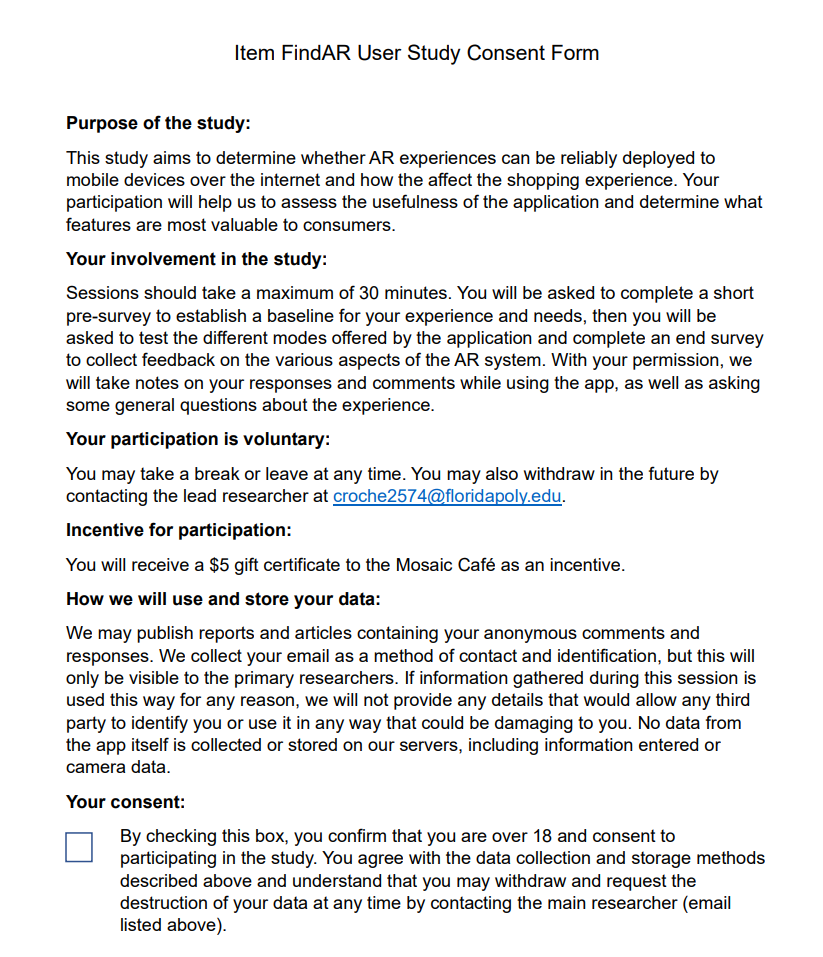
\includegraphics[width=0.85\linewidth]{Images/consent form.png}
    \caption{Original consent form}
    \label{fig:consent-form}
\end{figure}
\end{appendices}
\end{body}
\end{document}